%!TEX root = ../thesis.tex
\chapter{Appendix}
\label{chap:appendix}

The code for the Discrete Voter Model can be found in full in \href{https://github.com/hangulu/thesis}{this GitHub repository}.

That repository also contains notebooks to run and test the modules of DVM. To completely reproduce these experiments, run \texttt{mock\_experiments.ipynb} and \texttt{case\_experiments} in full.

The following are notable code snippets mentioned in the body of the article.

\newpage
\insertcode{"code/ei.py"}{Python Implementation of King's Ecological Inference}{lst:ei_code}

\newpage
\insertcode{"code/partition.py"}{Integer Partitioning}{lst:integer_partition}

\newpage
\section{Bar Plots Comparing Experiment Results For All Elections}
\label{sec:appendix_bars}

\FloatBarrier
\subsection{Runtime of $2 \times 2$ Cases}

\begin{figure}[ht]\centering
 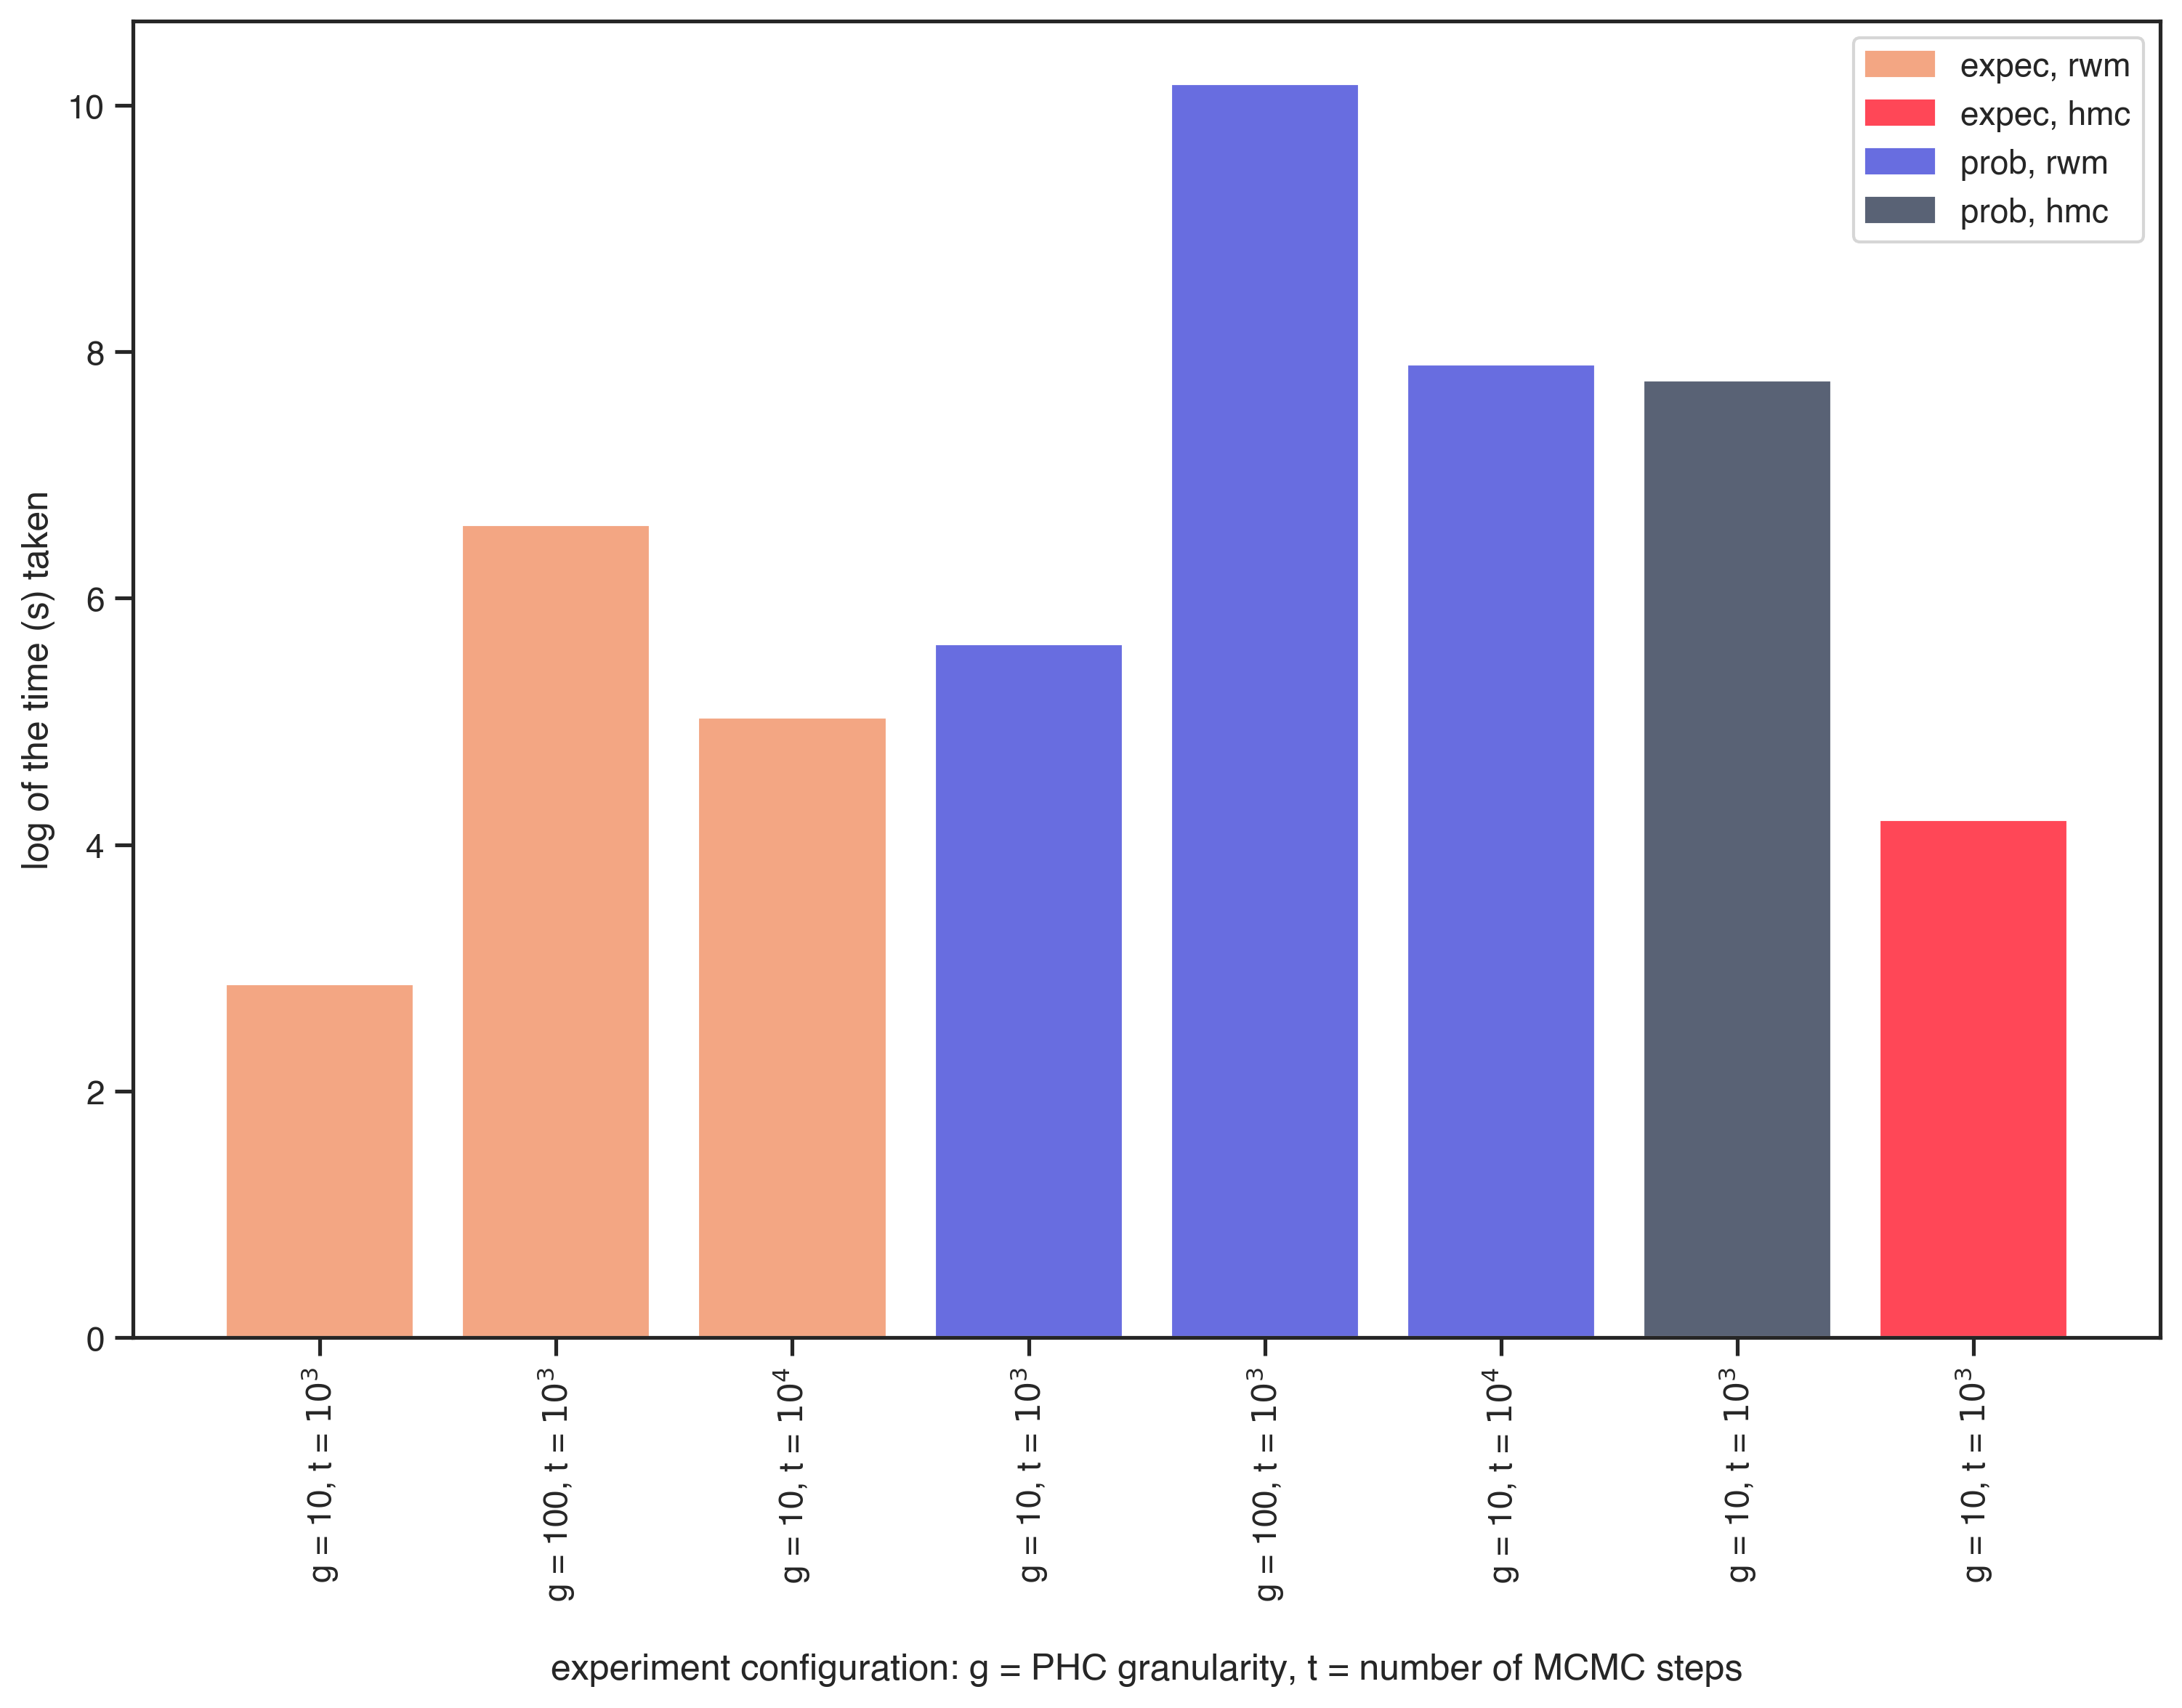
\includegraphics[width=0.75\linewidth]{figures/1_1_time.png}
 \caption{Runtime of the Configurations on the $d_1 \times v_1$ Election}
 \label{fig:1_1_time_append}
\end{figure}

\begin{figure}[ht]\centering
 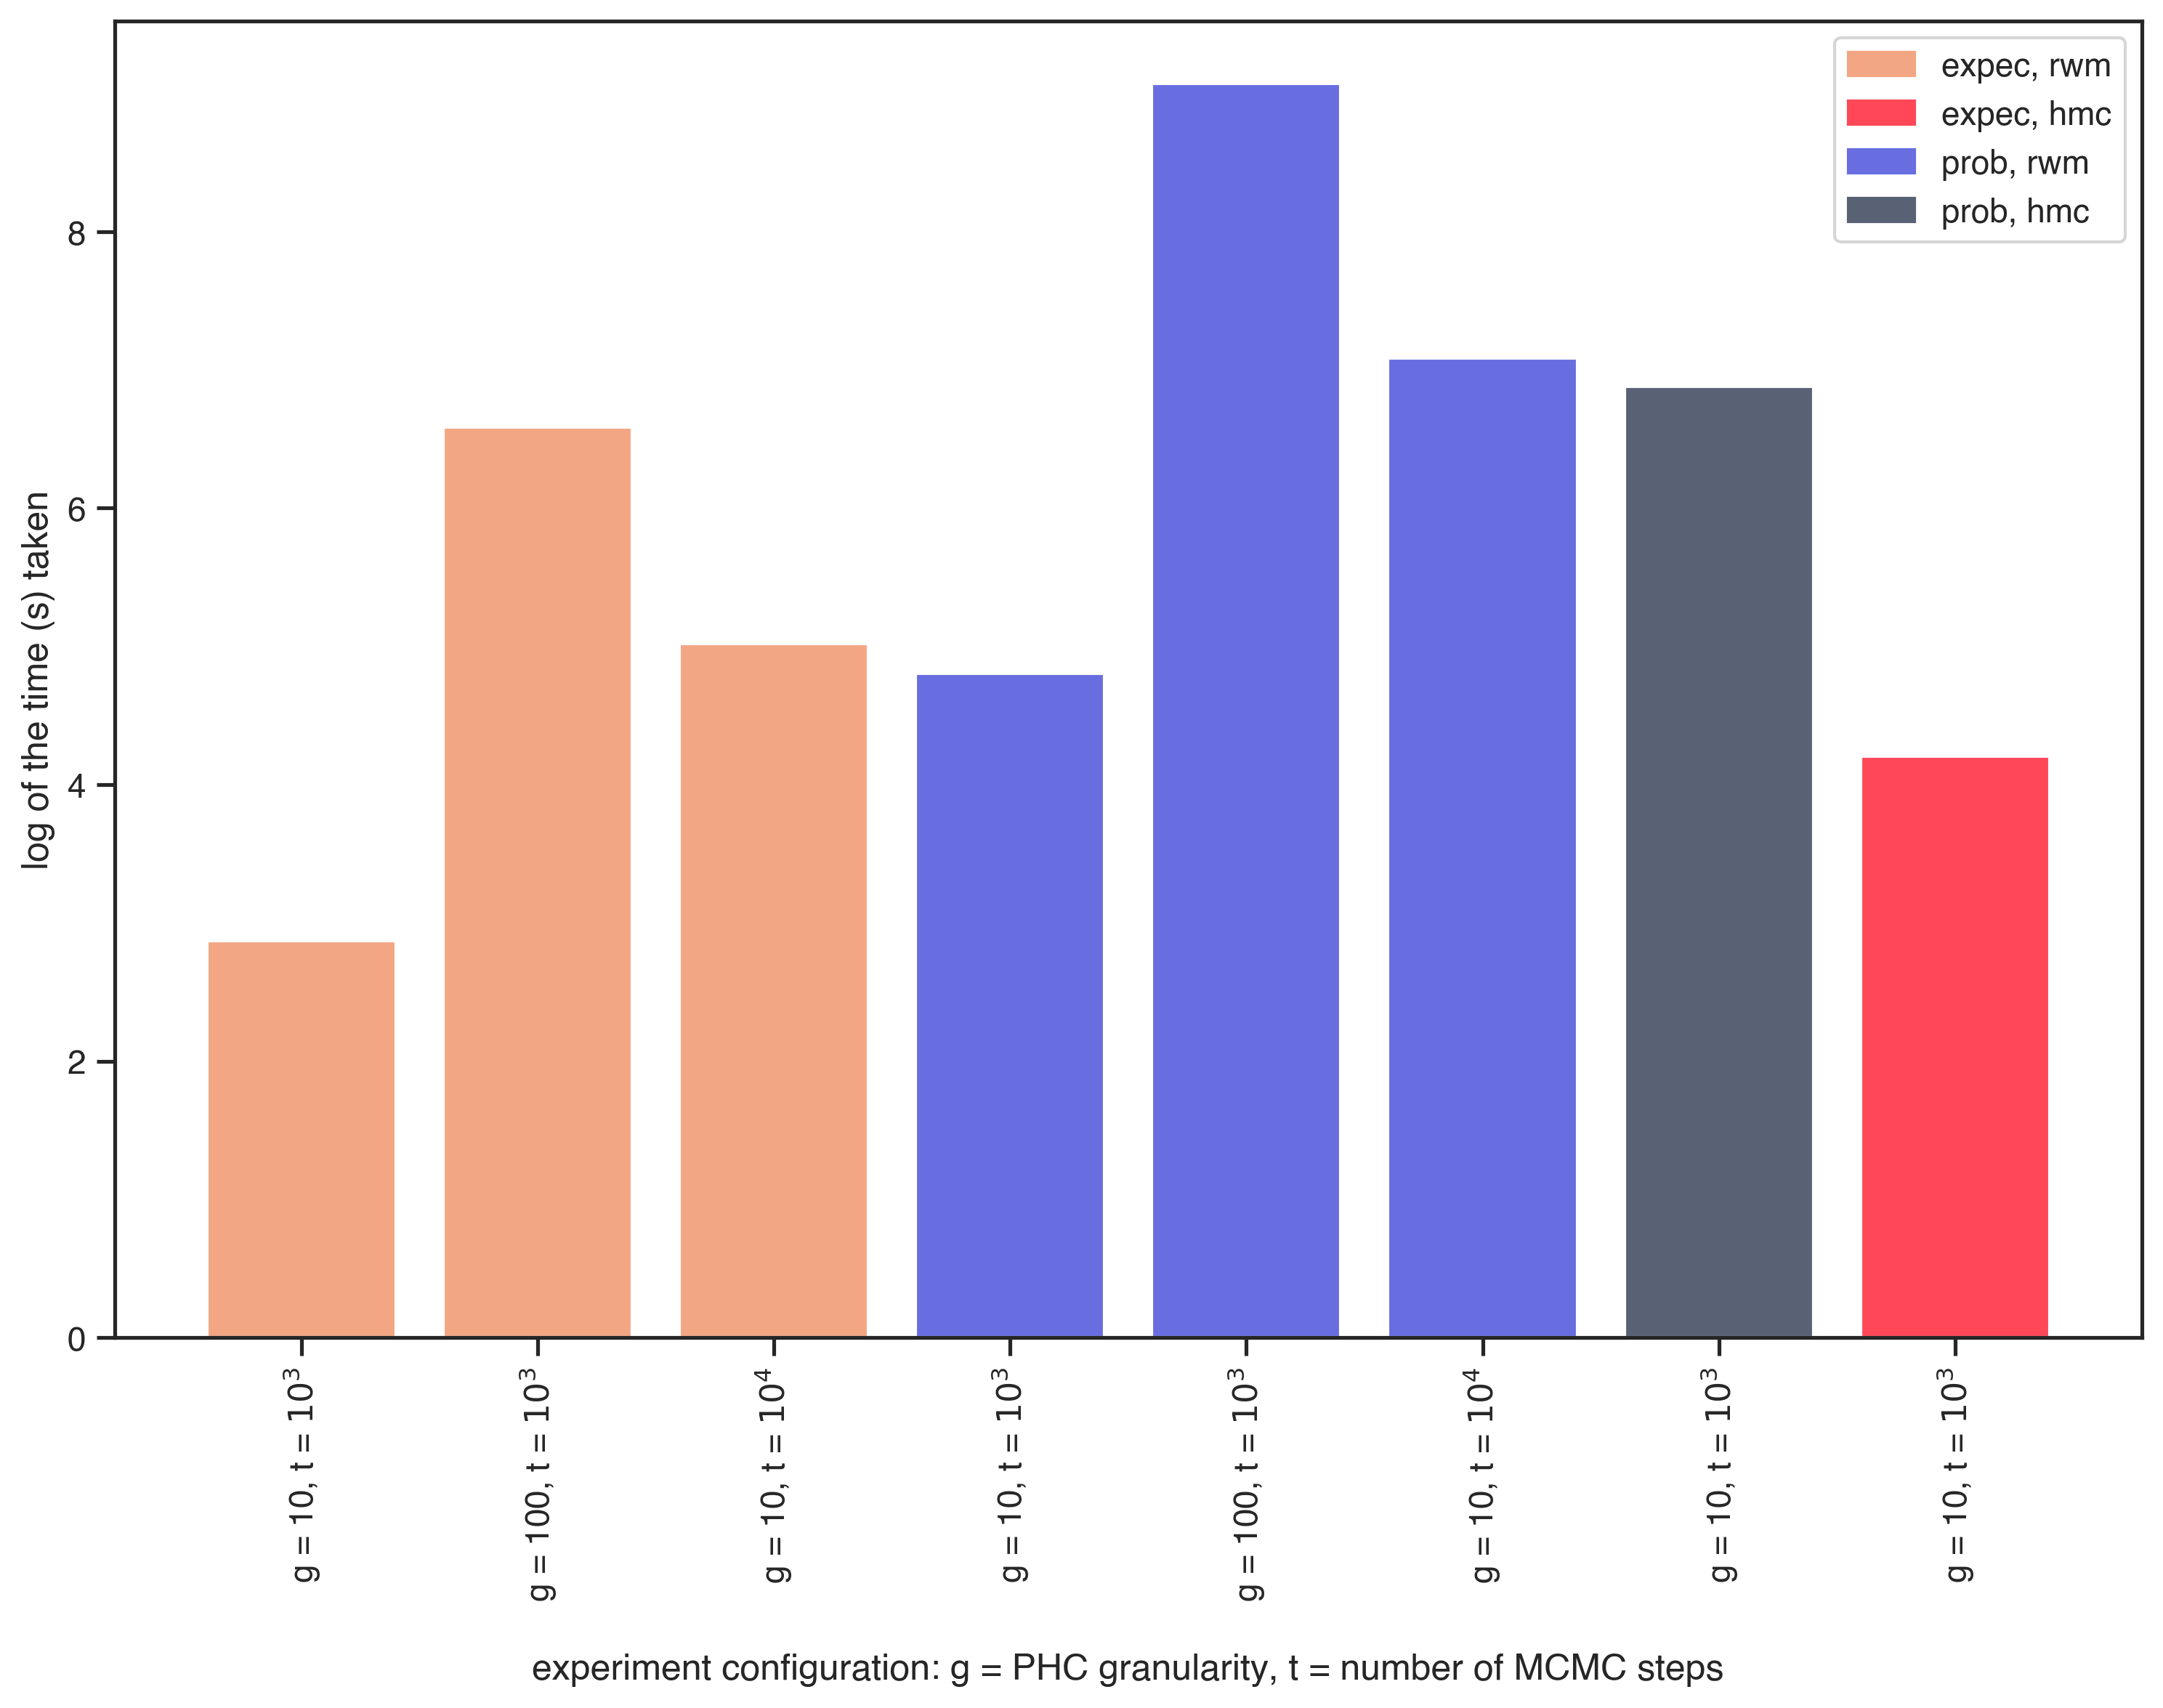
\includegraphics[width=0.75\linewidth]{figures/1_2_time.png}
 \caption{Runtime of the Configurations on the $d_1 \times v_2$ Election}
 \label{fig:1_2_time}
\end{figure}

\begin{figure}[ht]\centering
 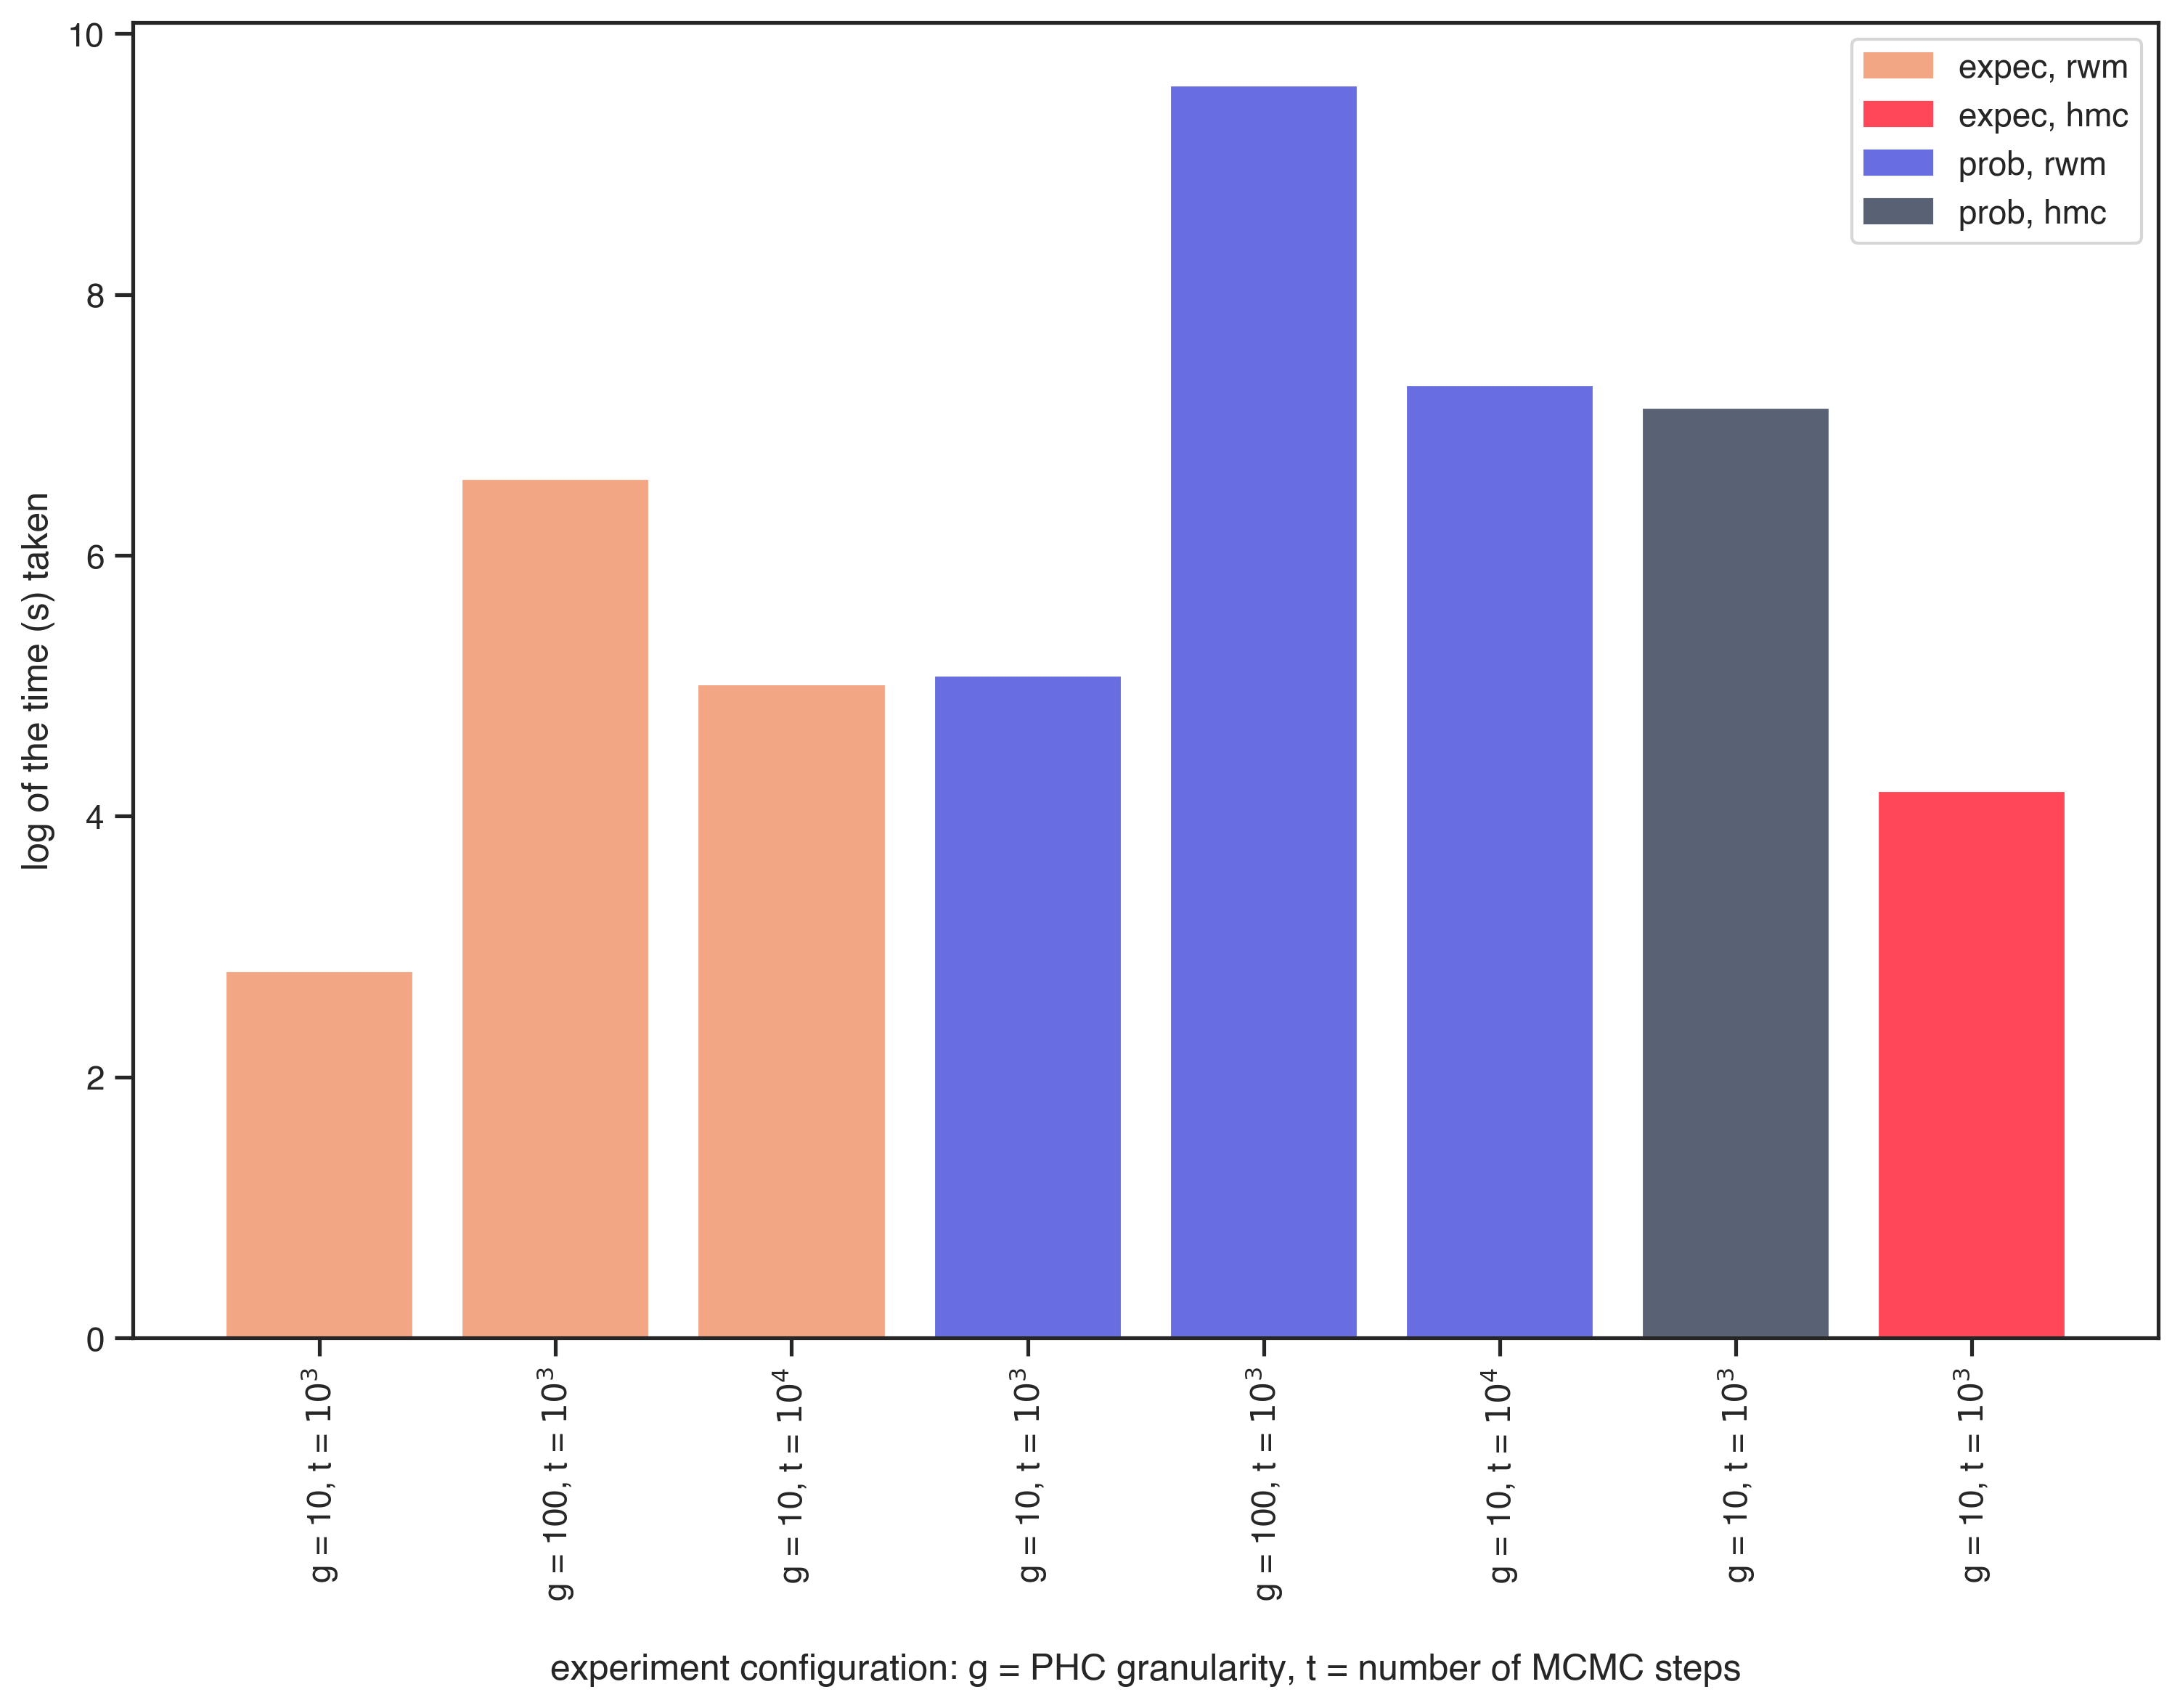
\includegraphics[width=0.75\linewidth]{figures/2_1_time.png}
 \caption{Runtime of the Configurations on the $d_2 \times v_1$ Election}
 \label{fig:2_1_time}
\end{figure}

\begin{figure}[ht]\centering
 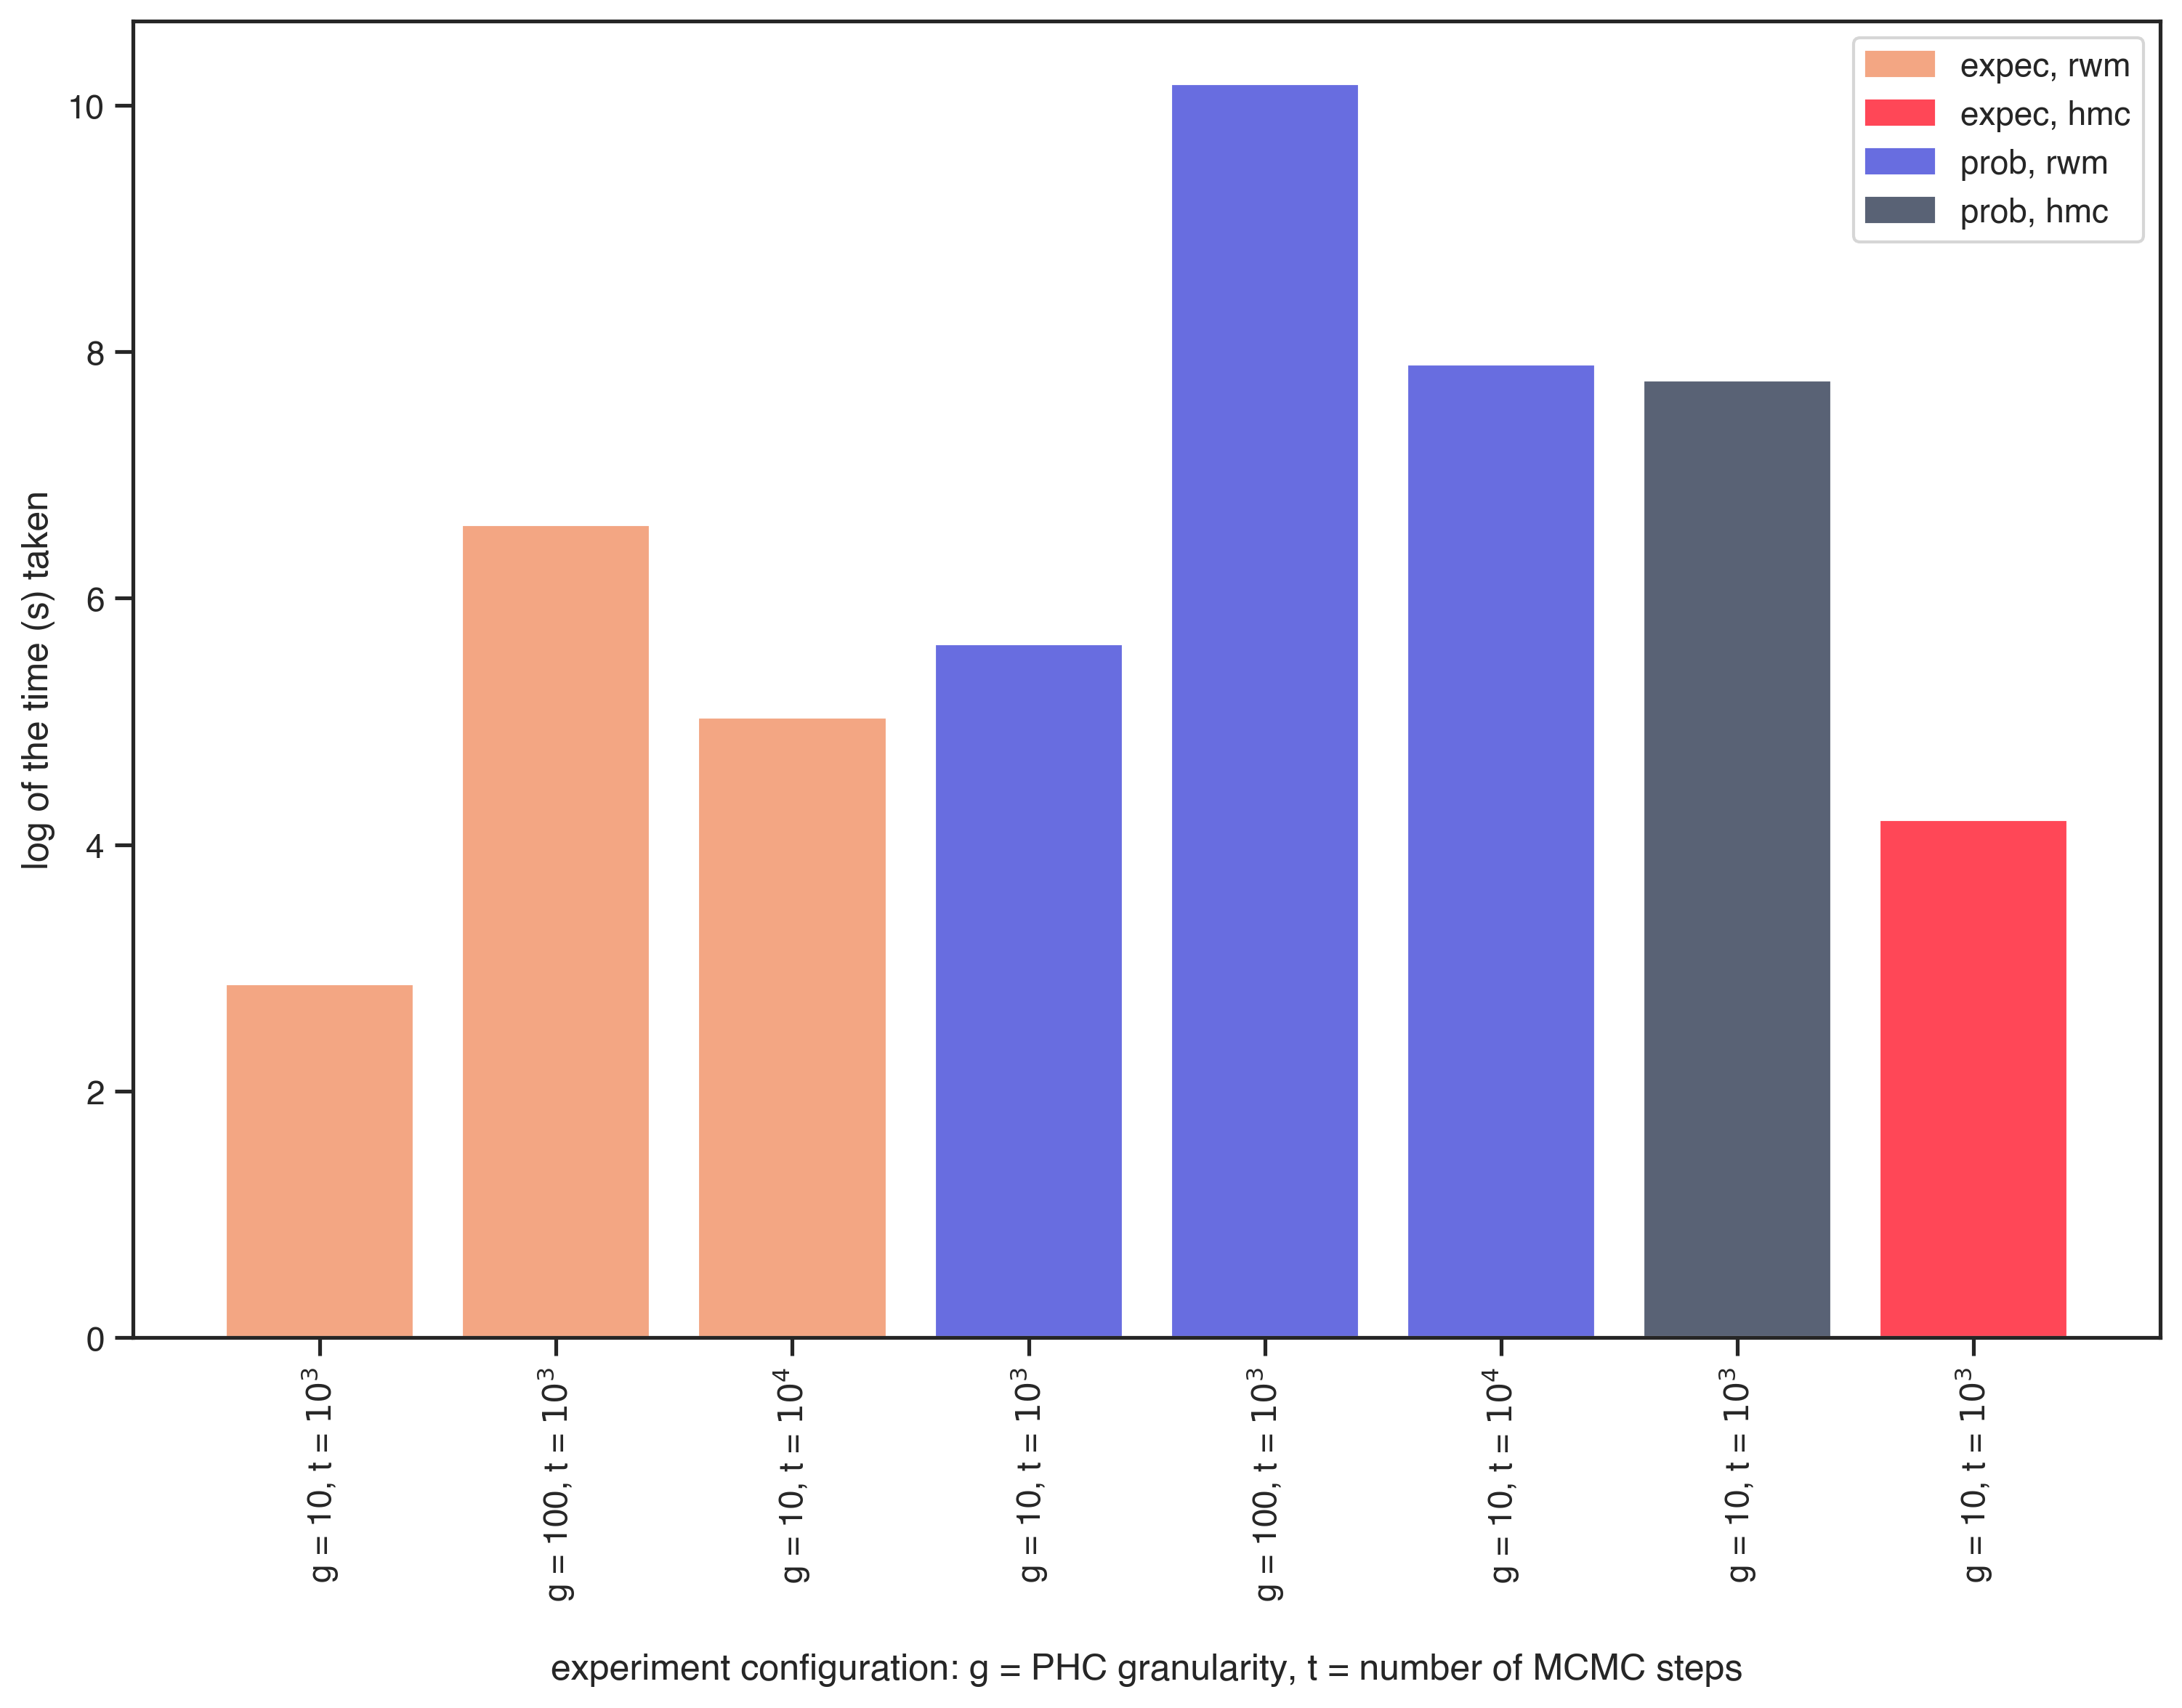
\includegraphics[width=0.75\linewidth]{figures/1_1_time.png}
 \caption{Runtime of the Configurations on the $d_2 \times v_2$ Election}
 \label{fig:2_2_time}
\end{figure}

\begin{figure}[ht]\centering
 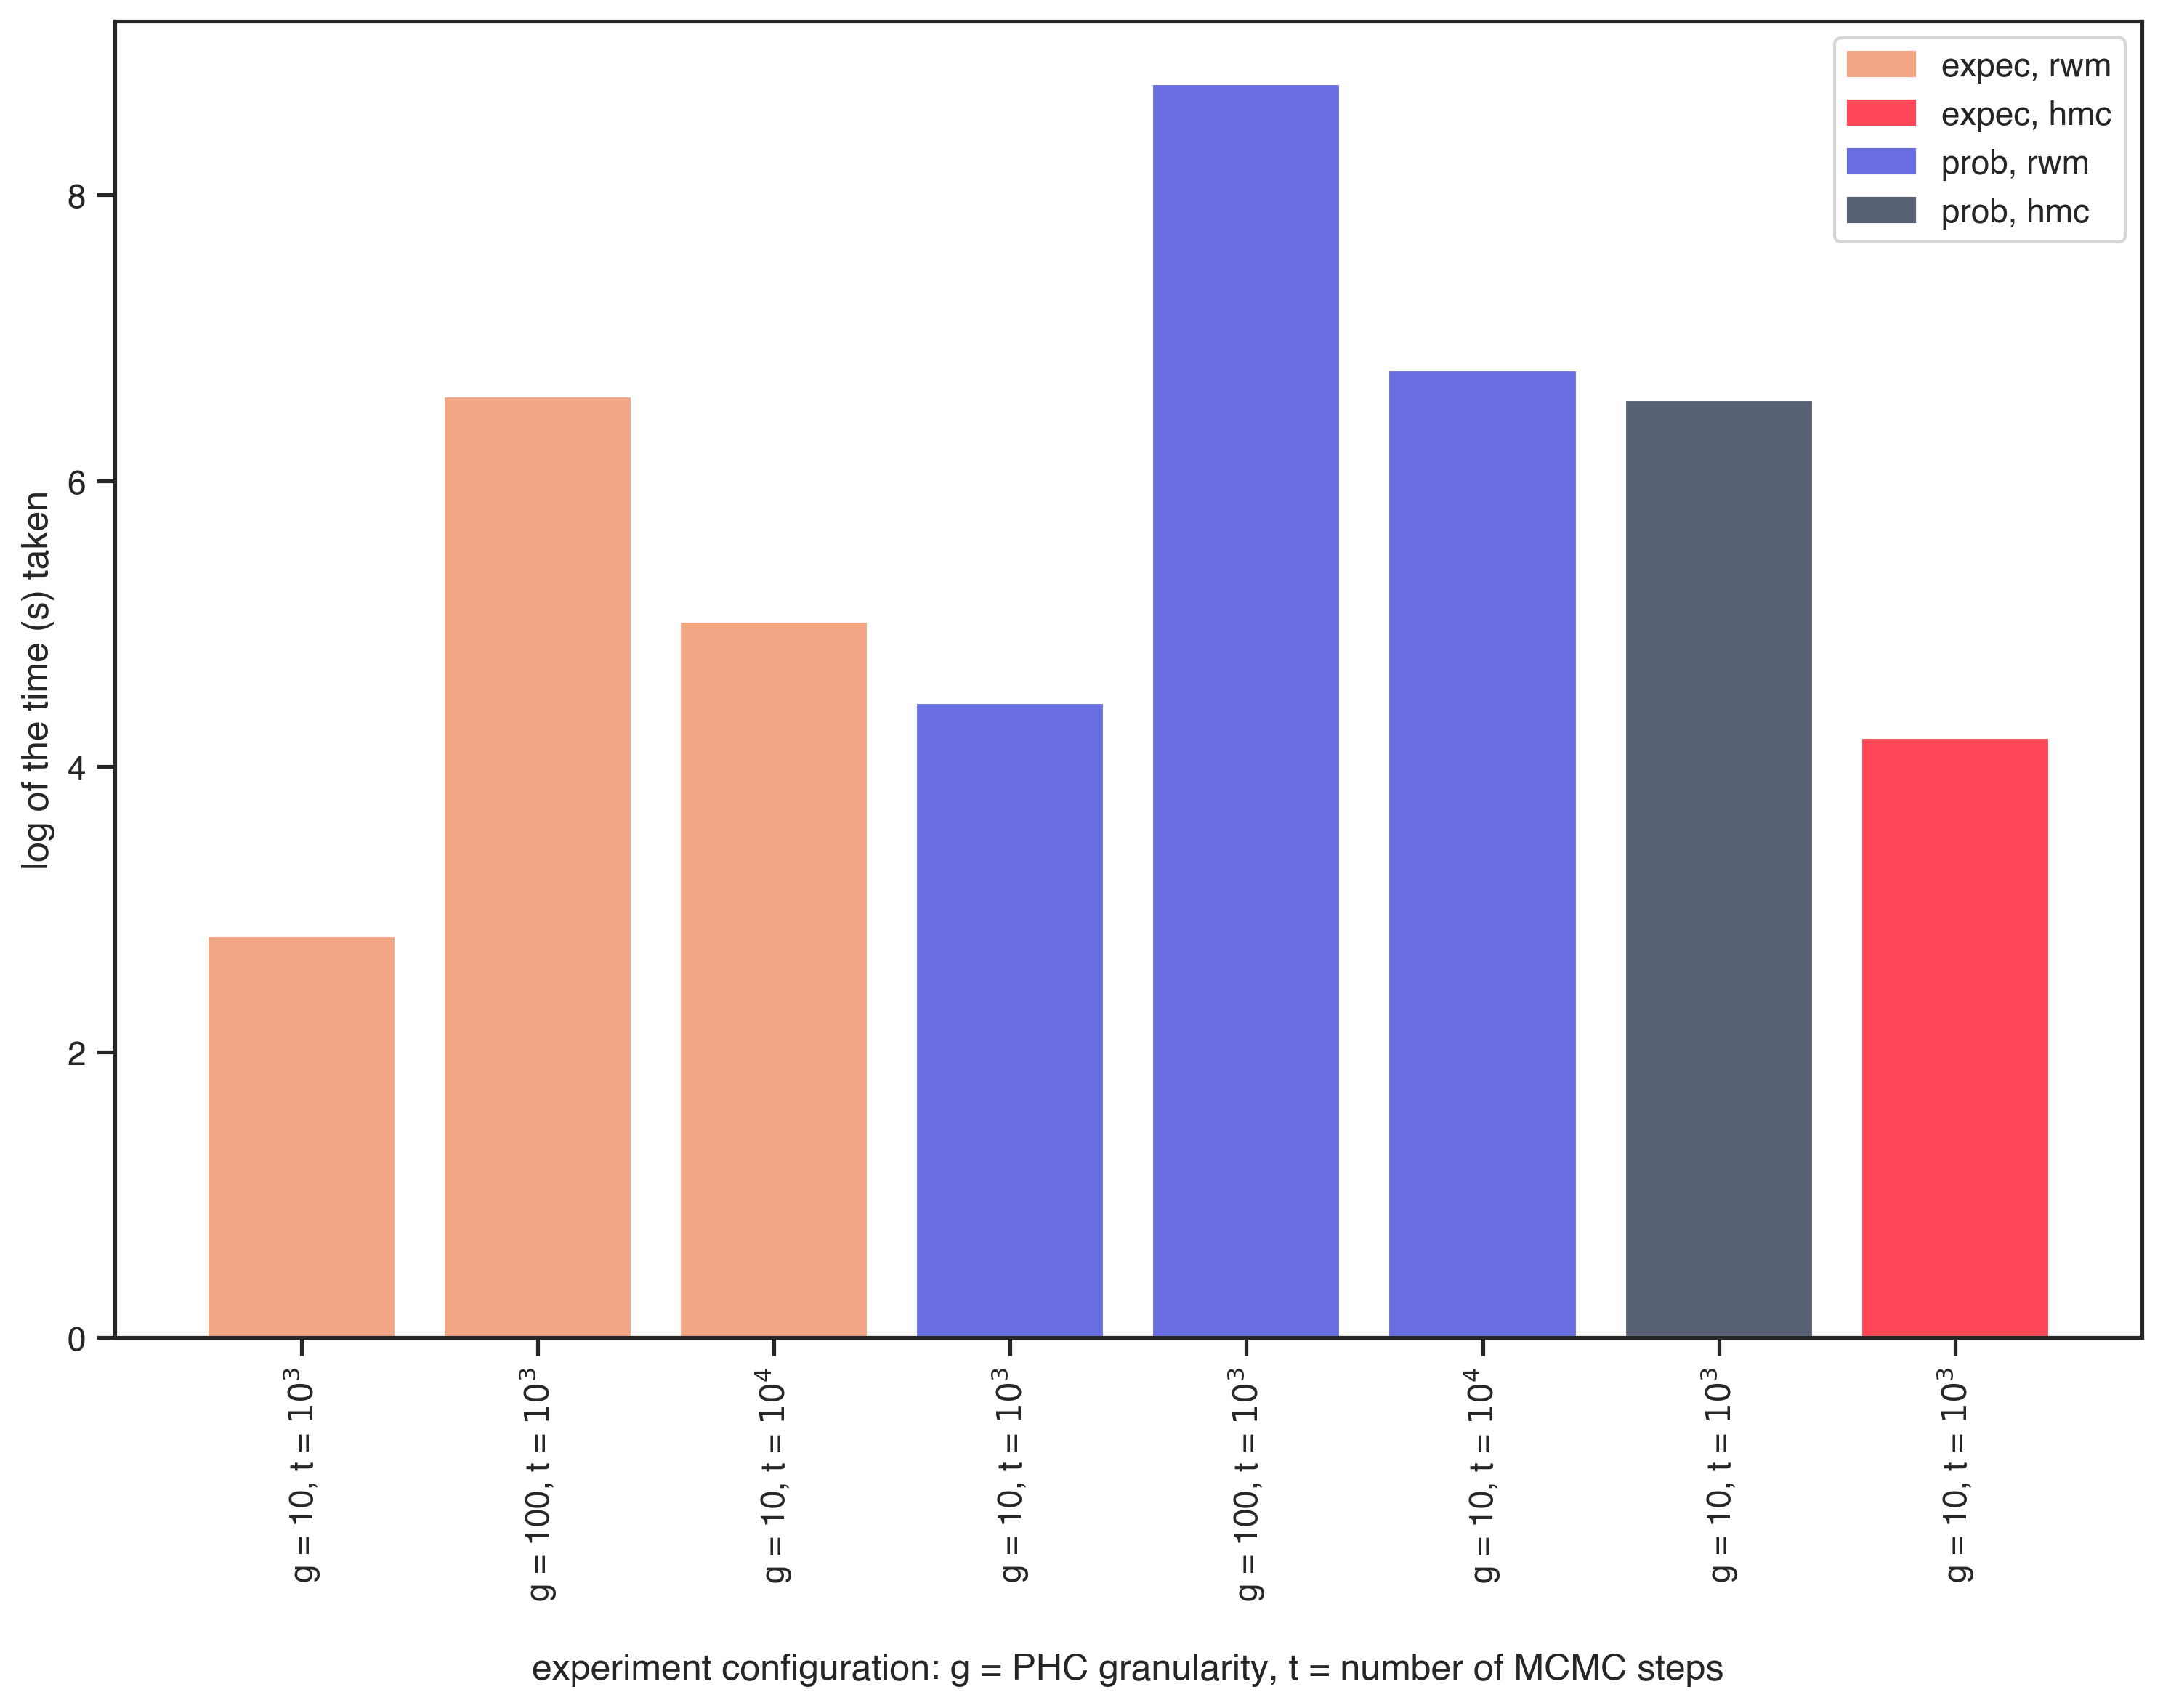
\includegraphics[width=0.75\linewidth]{figures/3_1_time.png}
 \caption{Runtime of the Configurations on the $d_3 \times v_1$ Election}
 \label{fig:3_1_time}
\end{figure}

\begin{figure}[ht]\centering
 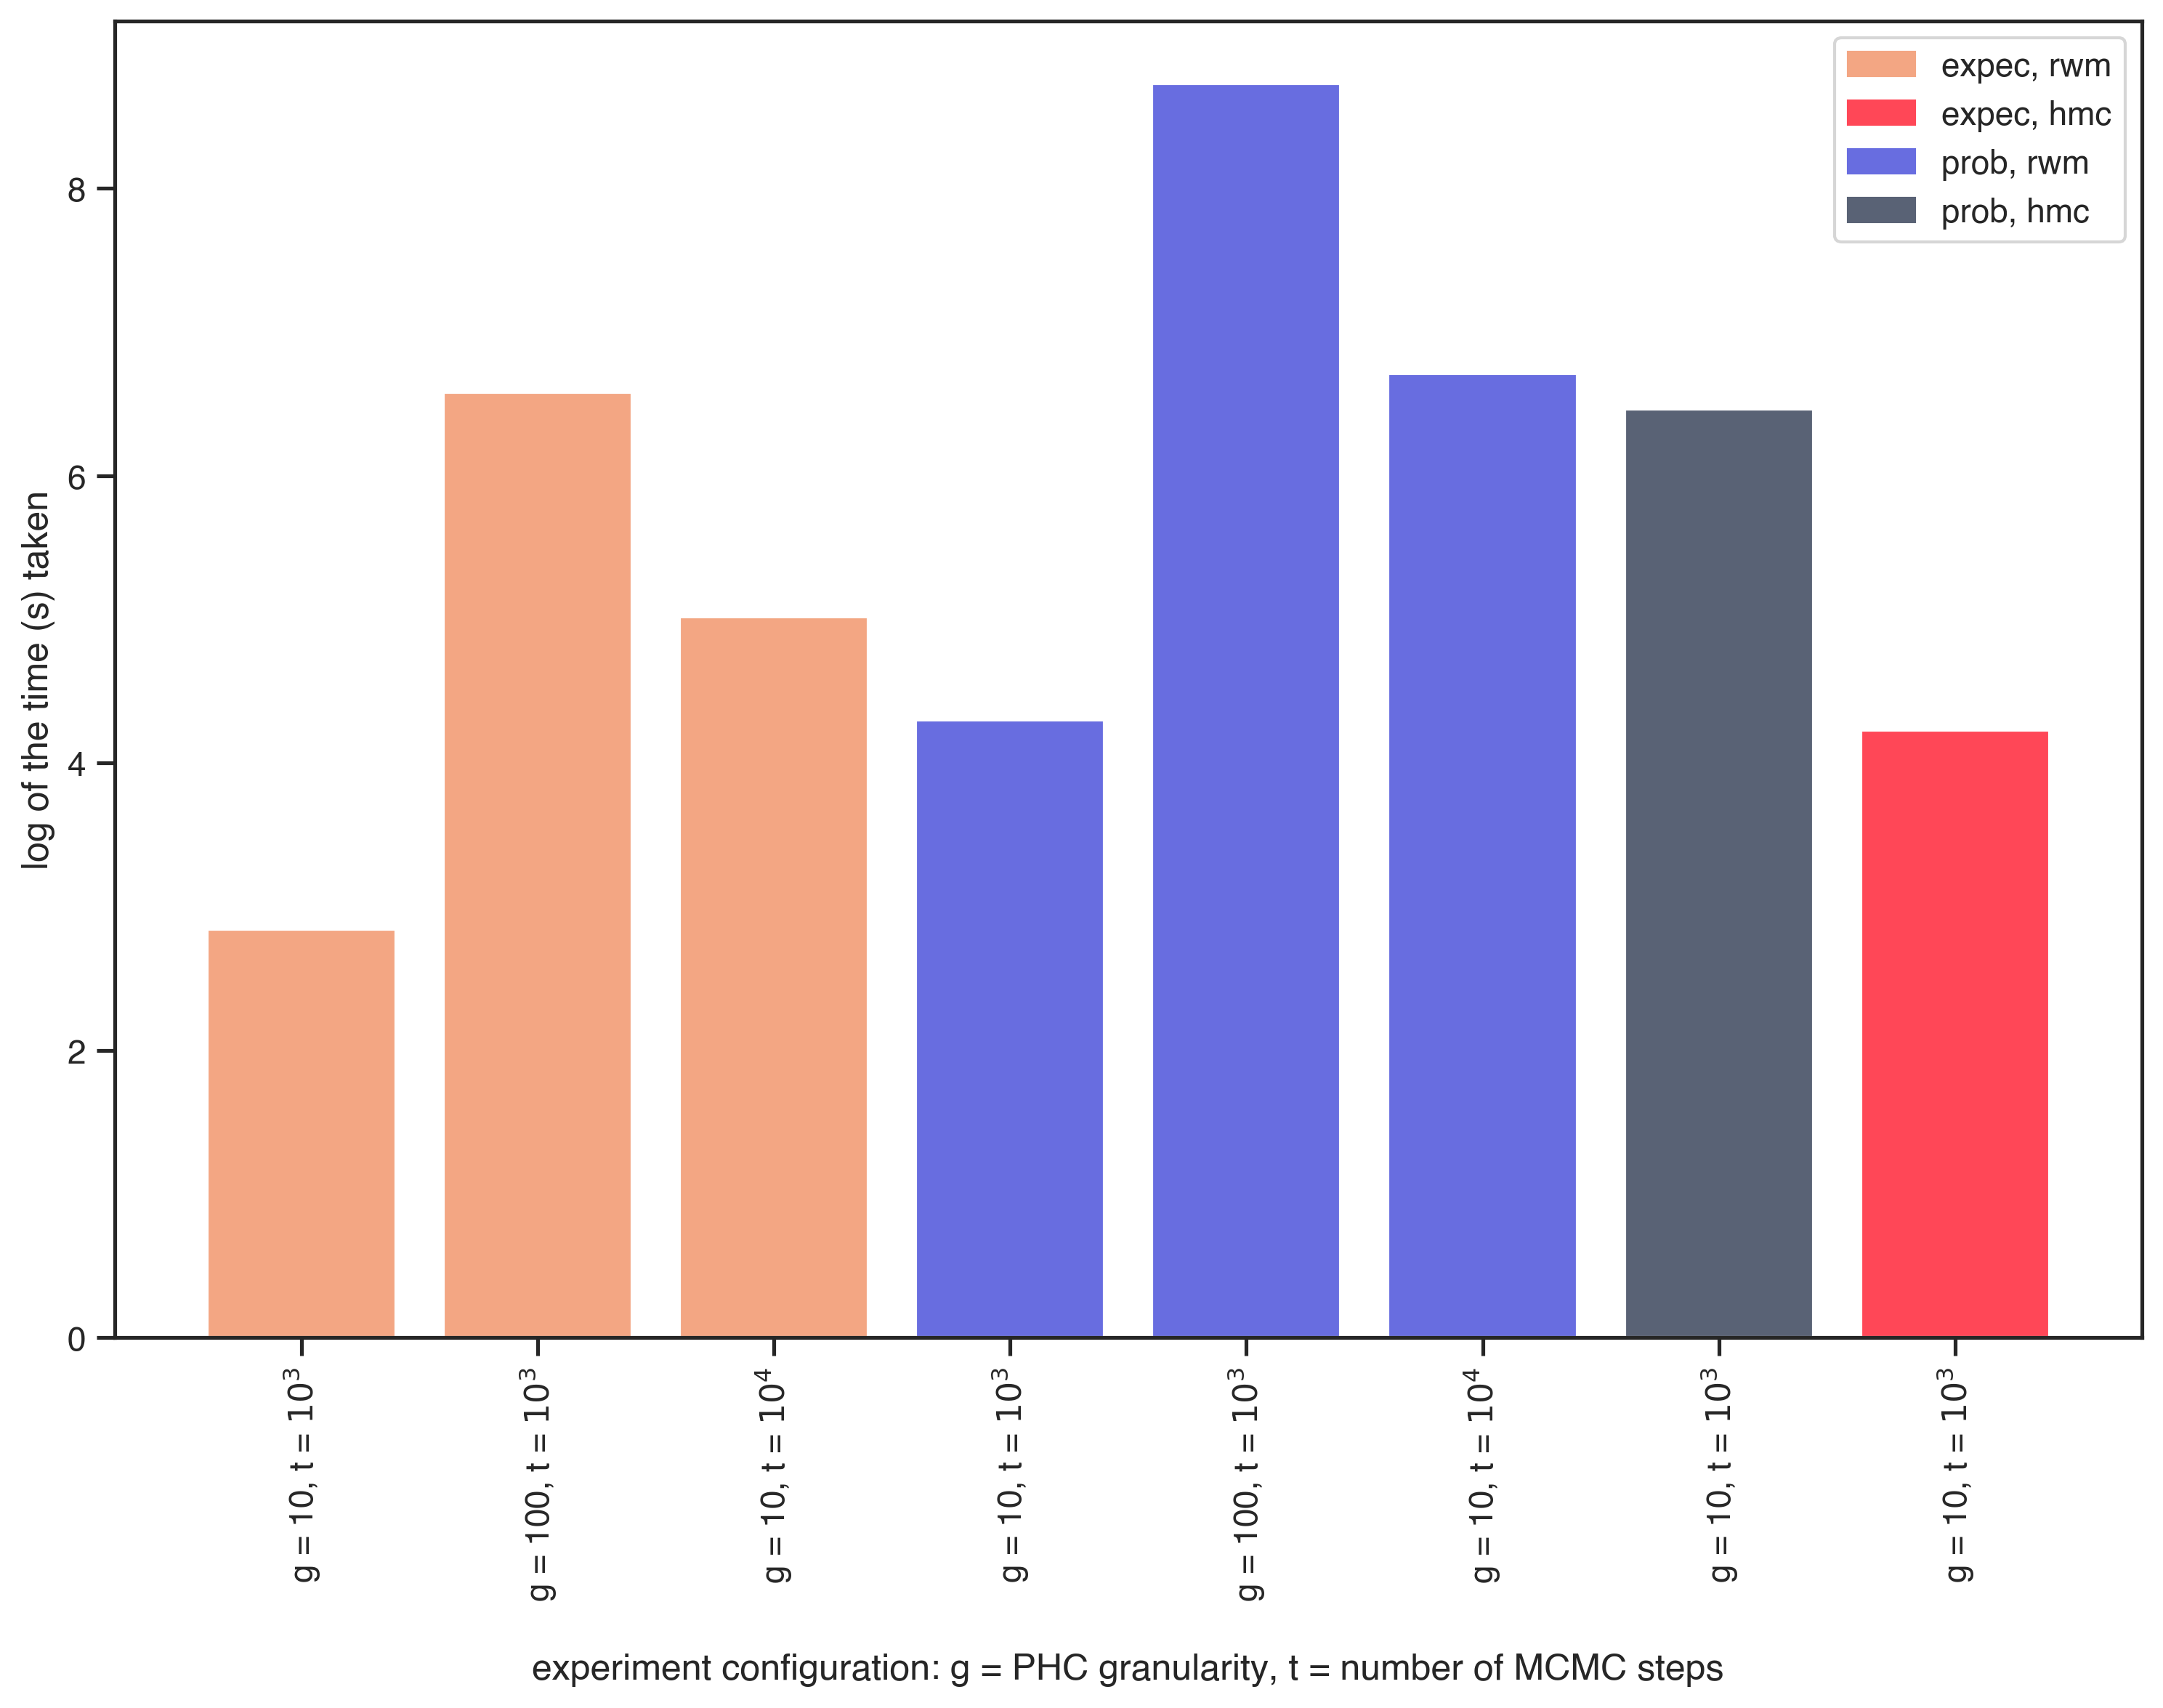
\includegraphics[width=0.75\linewidth]{figures/3_2_time.png}
 \caption{Runtime of the Configurations on the $d_3 \times v_2$ Election}
 \label{fig:3_2_time}
\end{figure}

\FloatBarrier
\subsection{Mean PHC MSE of $2 \times 2$ Cases}

\begin{figure}[ht]\centering
 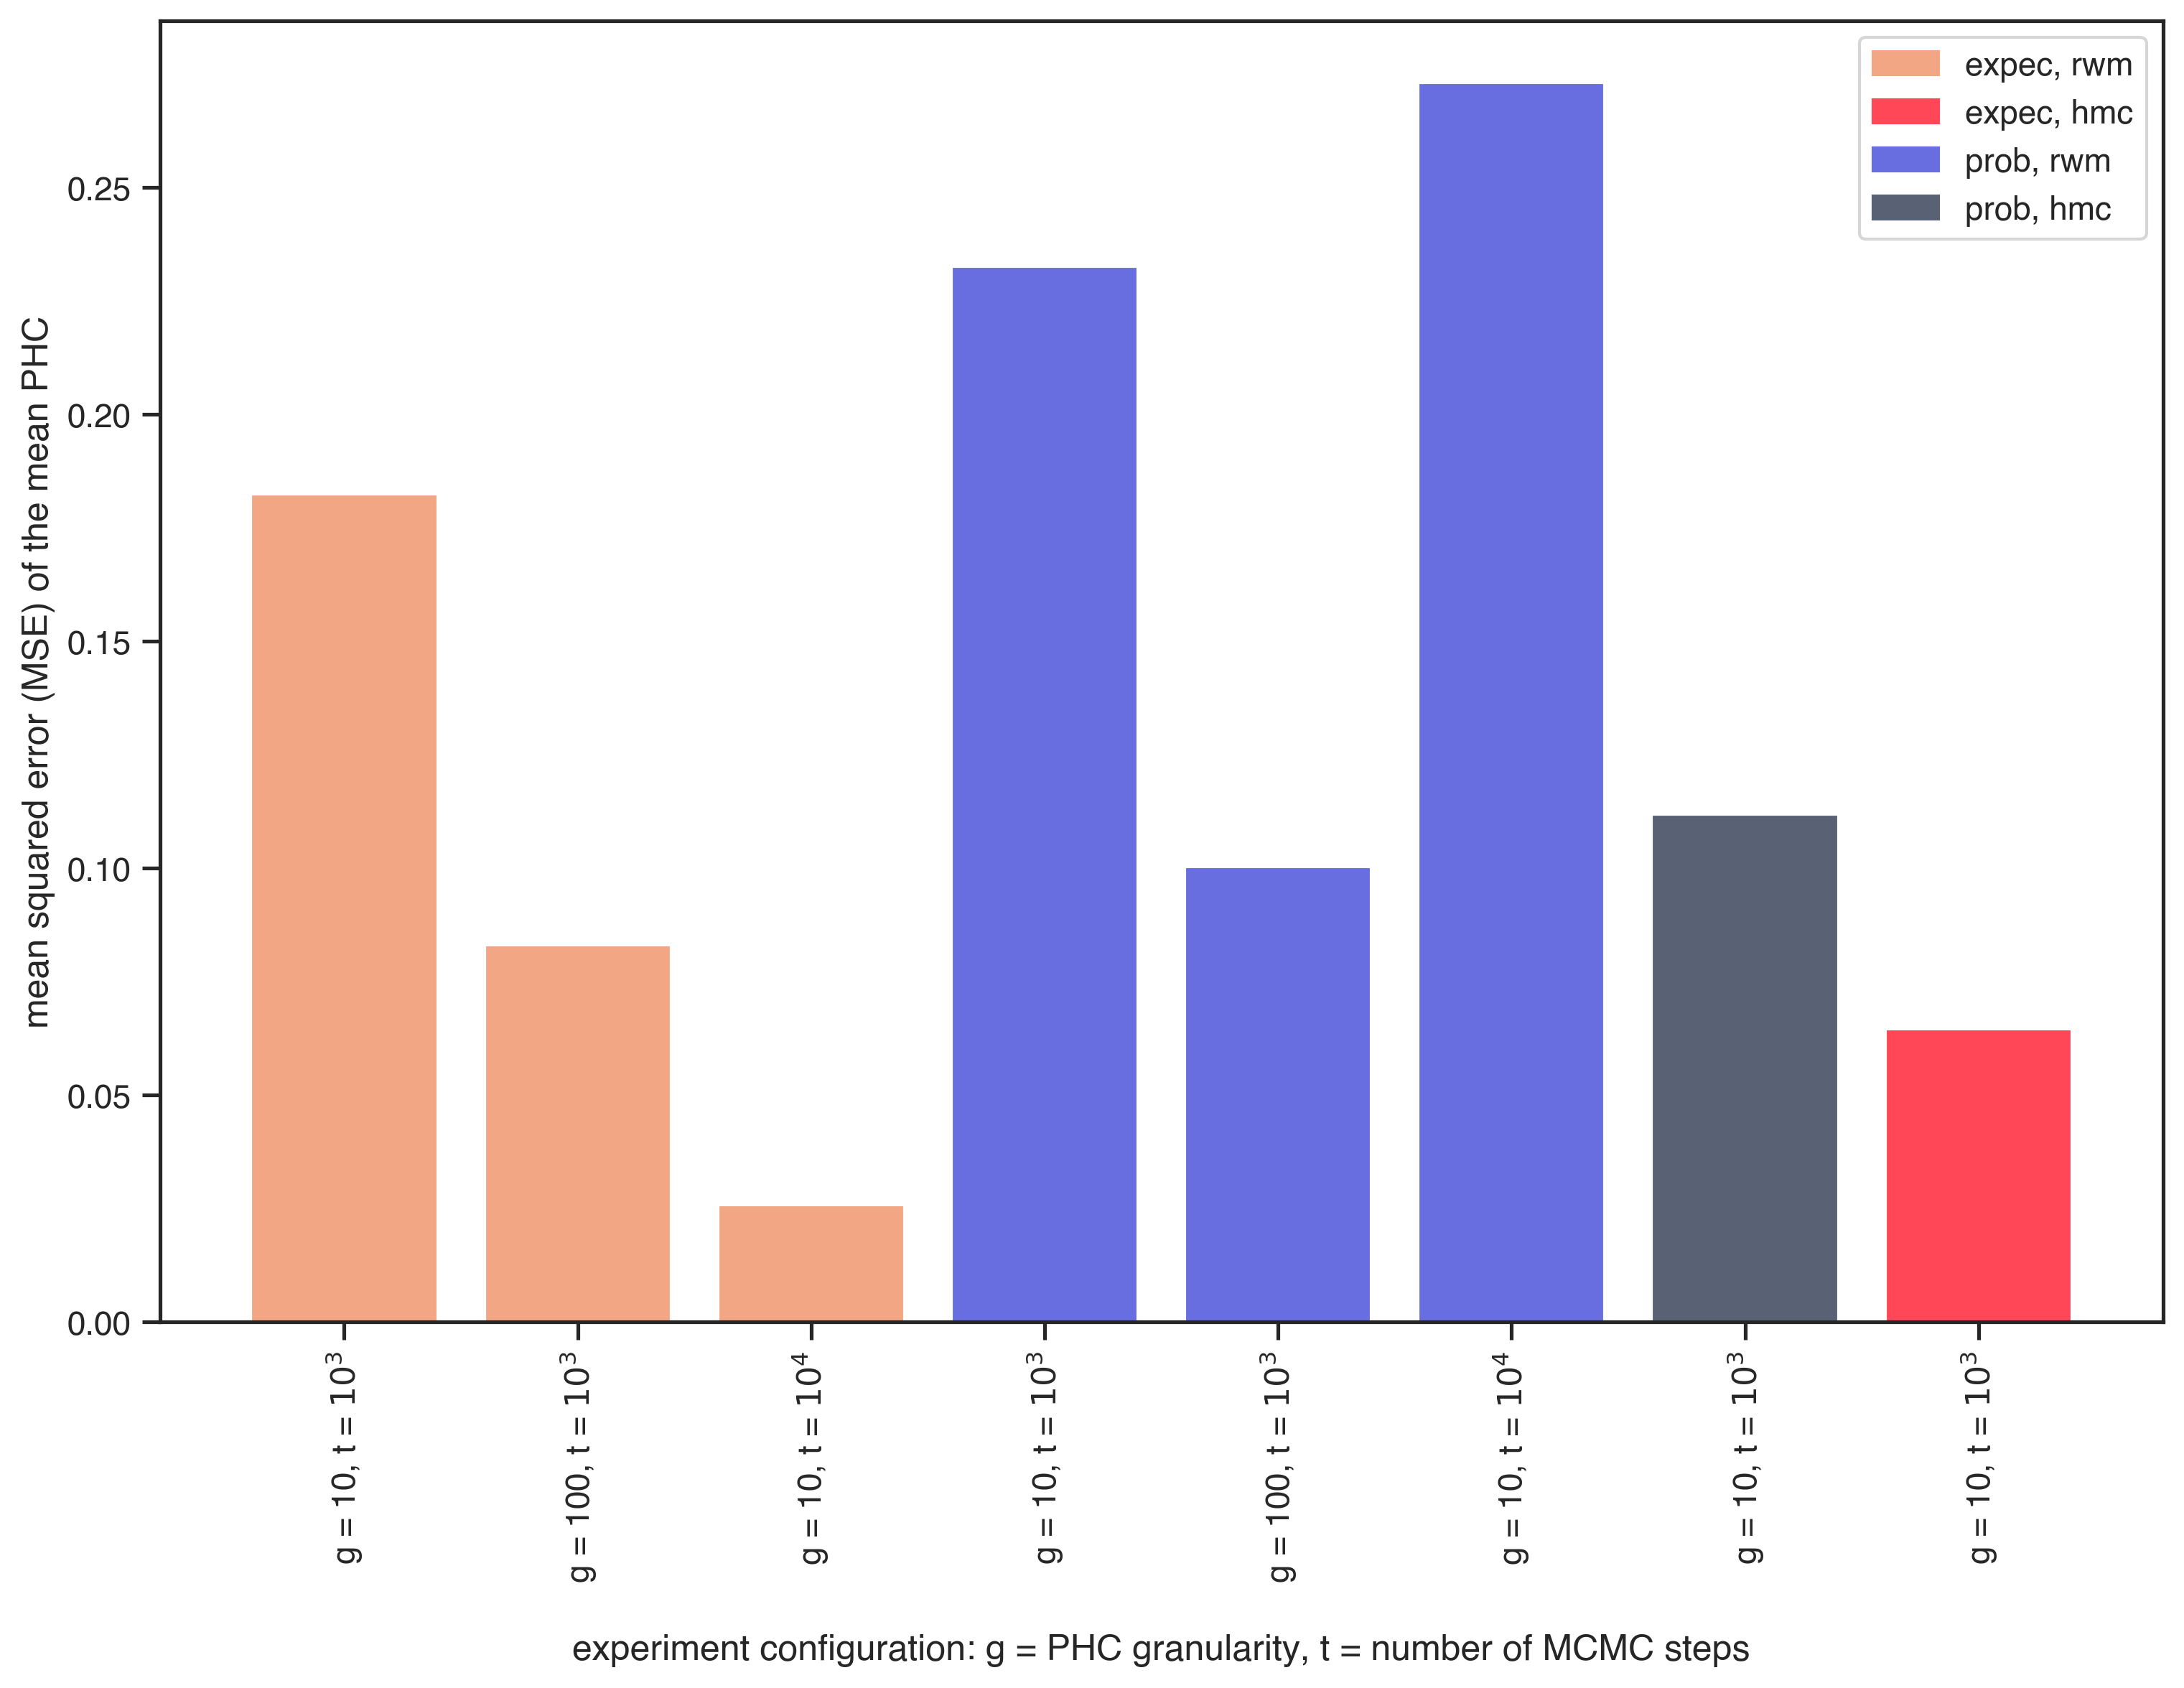
\includegraphics[width=0.75\linewidth]{figures/1_1_mean_mse.png}
 \caption{MSE of the Mean PHC of the Configurations' DVM on the $d_1 \times v_1$ Election}
 \label{fig:1_1_mean_mse_append}
\end{figure}

\begin{figure}[ht]\centering
 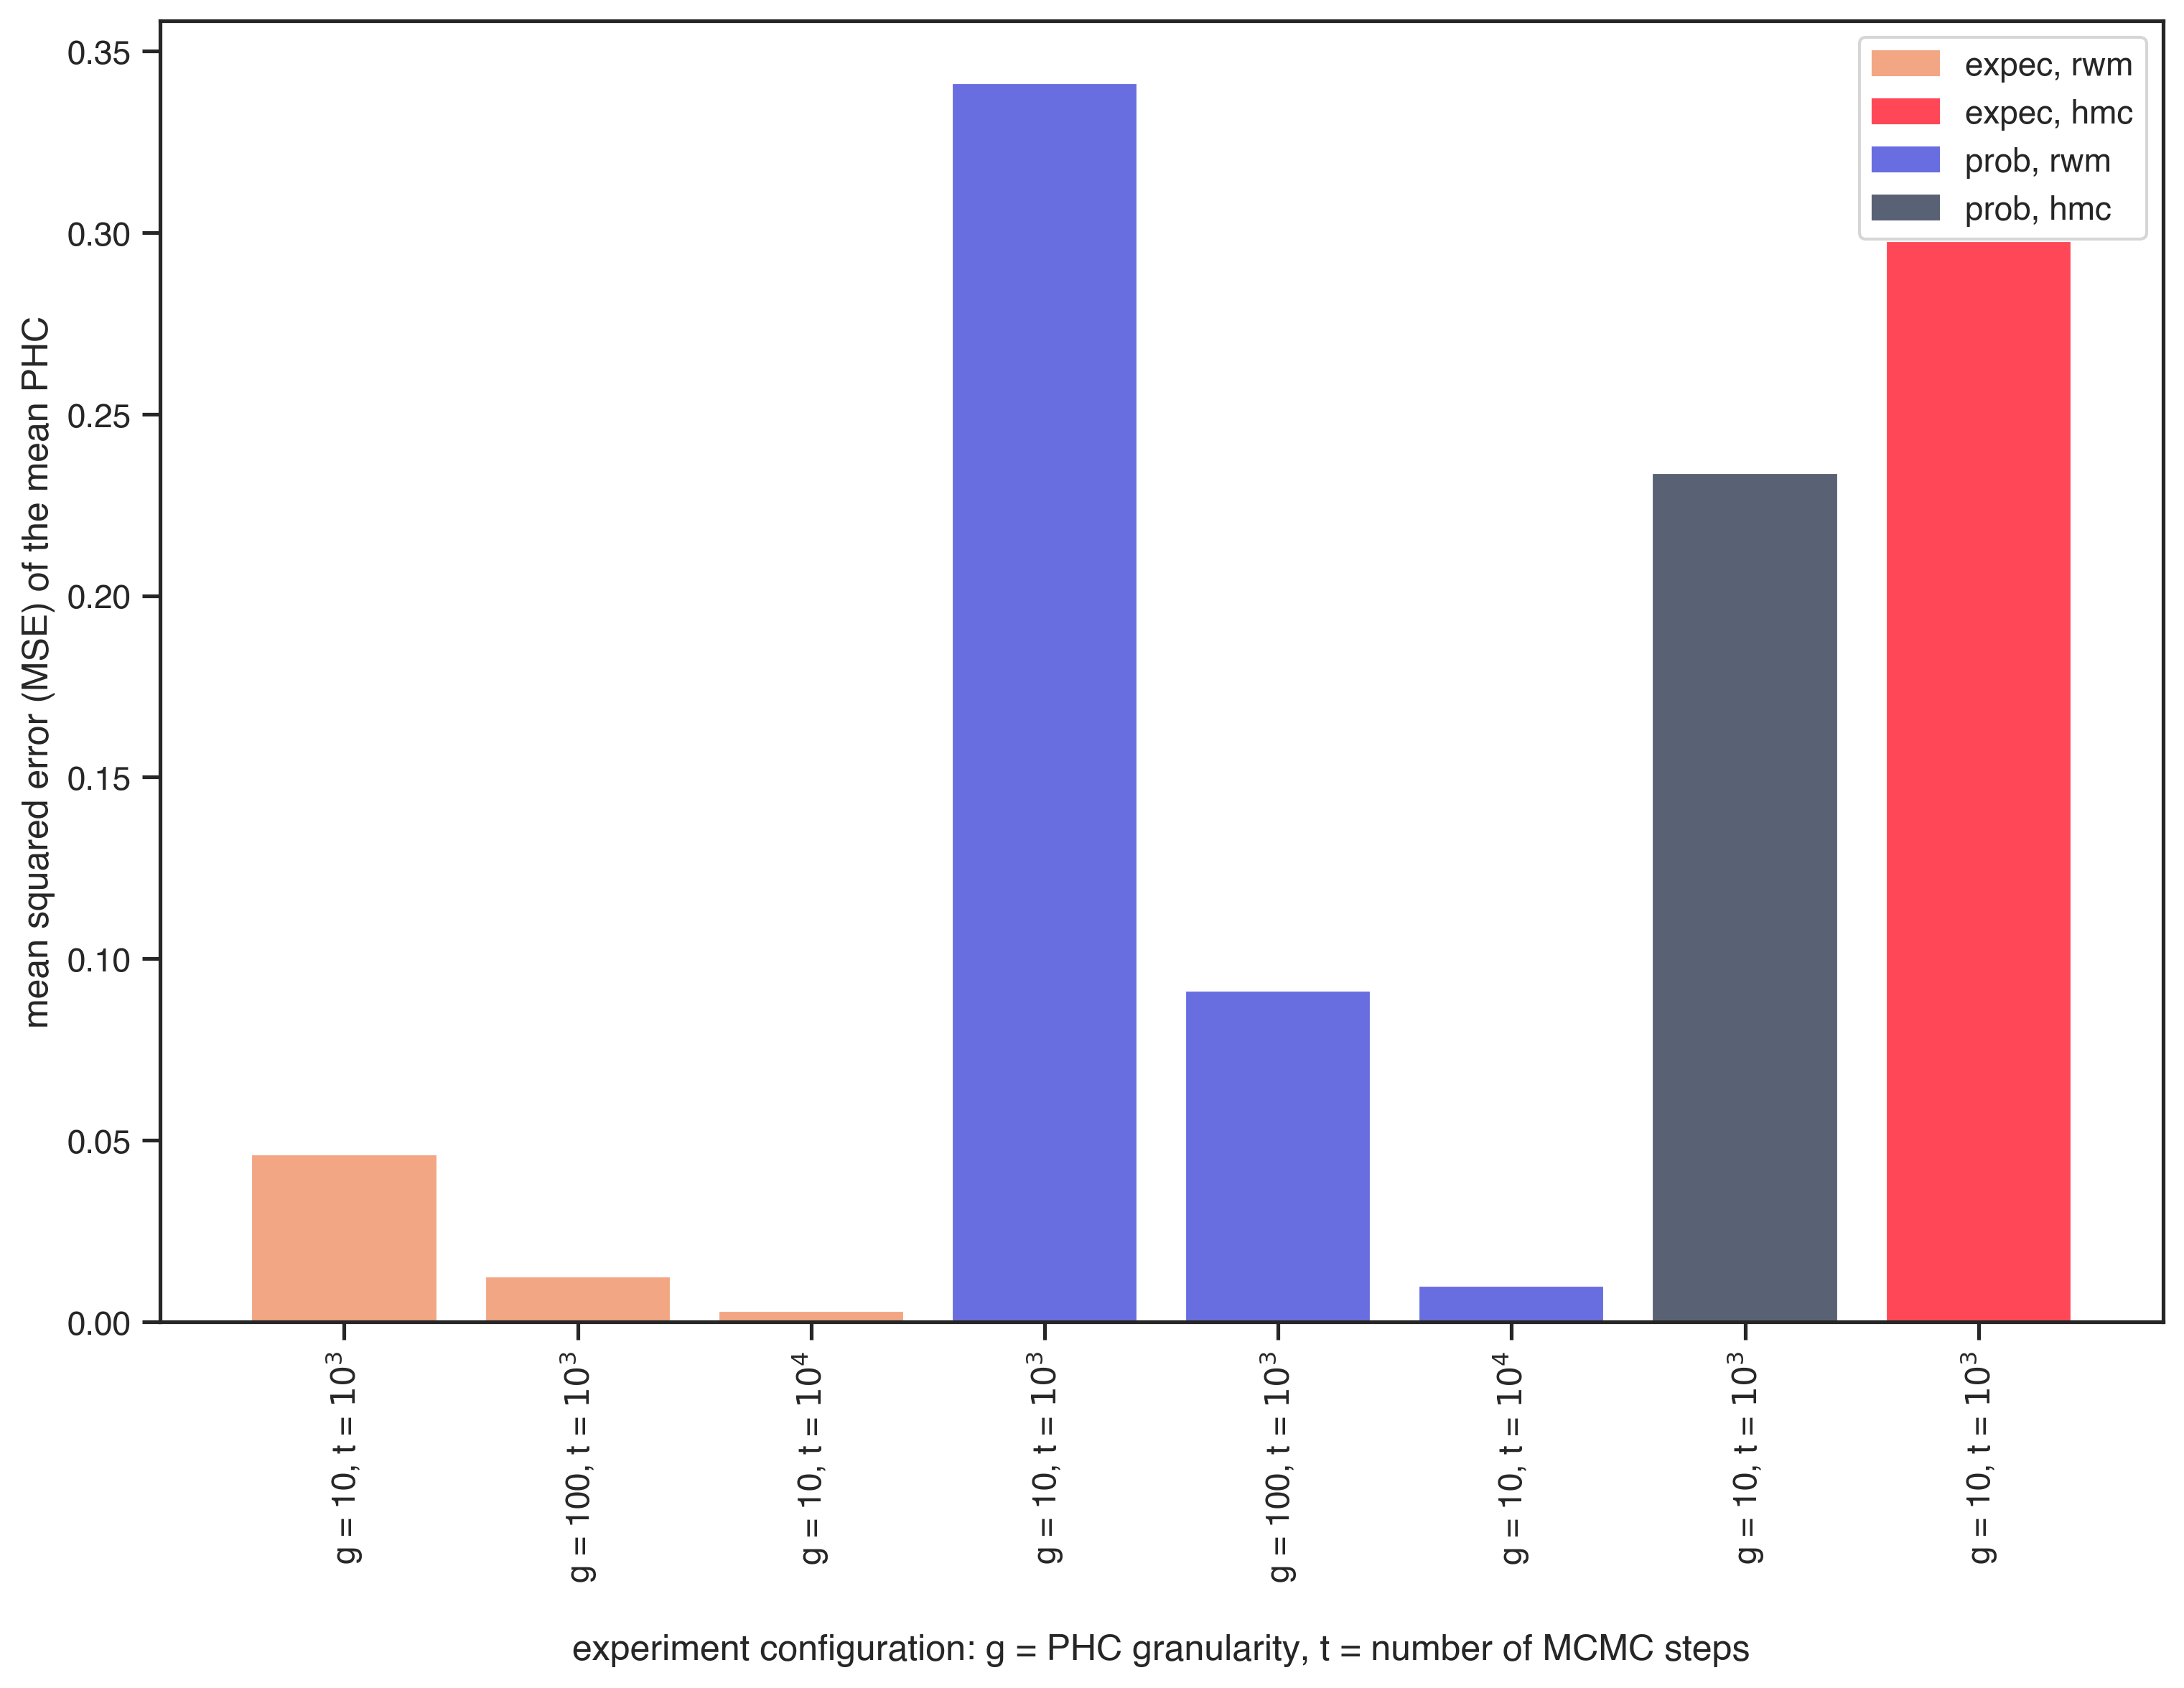
\includegraphics[width=0.75\linewidth]{figures/1_2_mean_mse.png}
 \caption{MSE of the Mean PHC of the Configurations' DVM on the $d_1 \times v_2$ Election}
 \label{fig:1_2_mean_mse}
\end{figure}

\begin{figure}[ht]\centering
 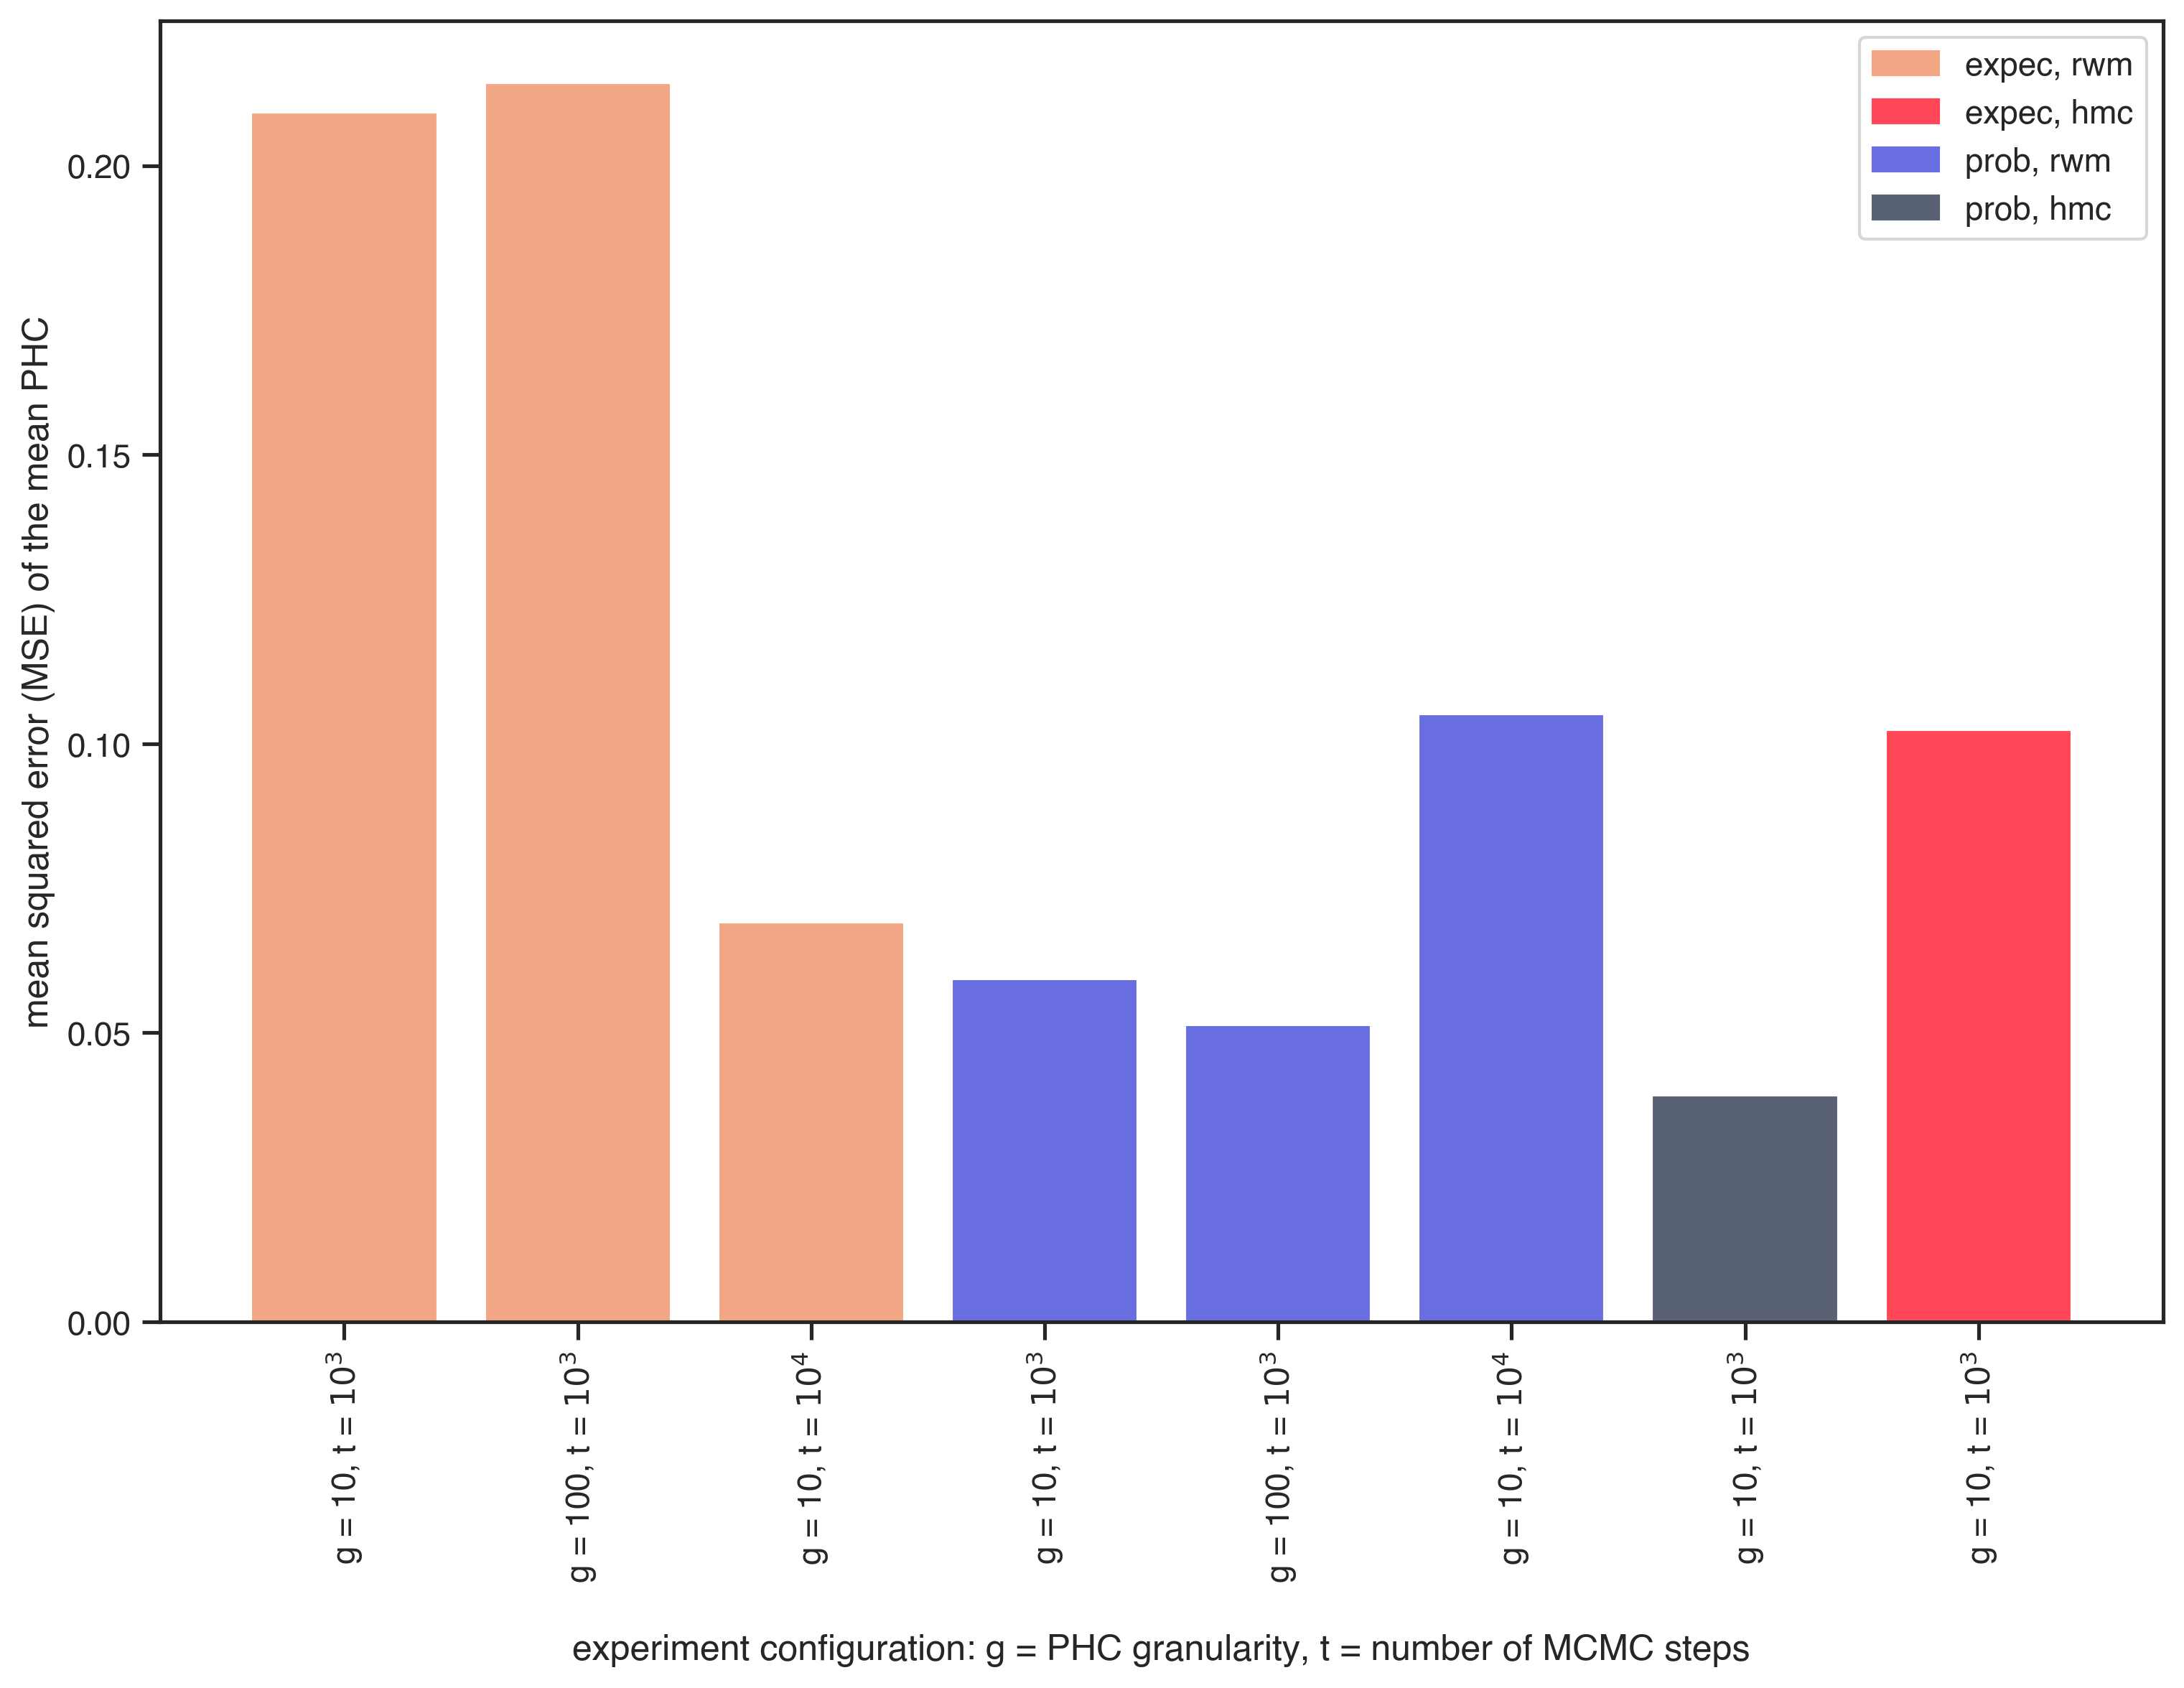
\includegraphics[width=0.75\linewidth]{figures/2_1_mean_mse.png}
 \caption{MSE of the Mean PHC of the Configurations' DVM on the $d_2 \times v_1$ Election}
 \label{fig:2_1_mean_mse}
\end{figure}

\begin{figure}[ht]\centering
 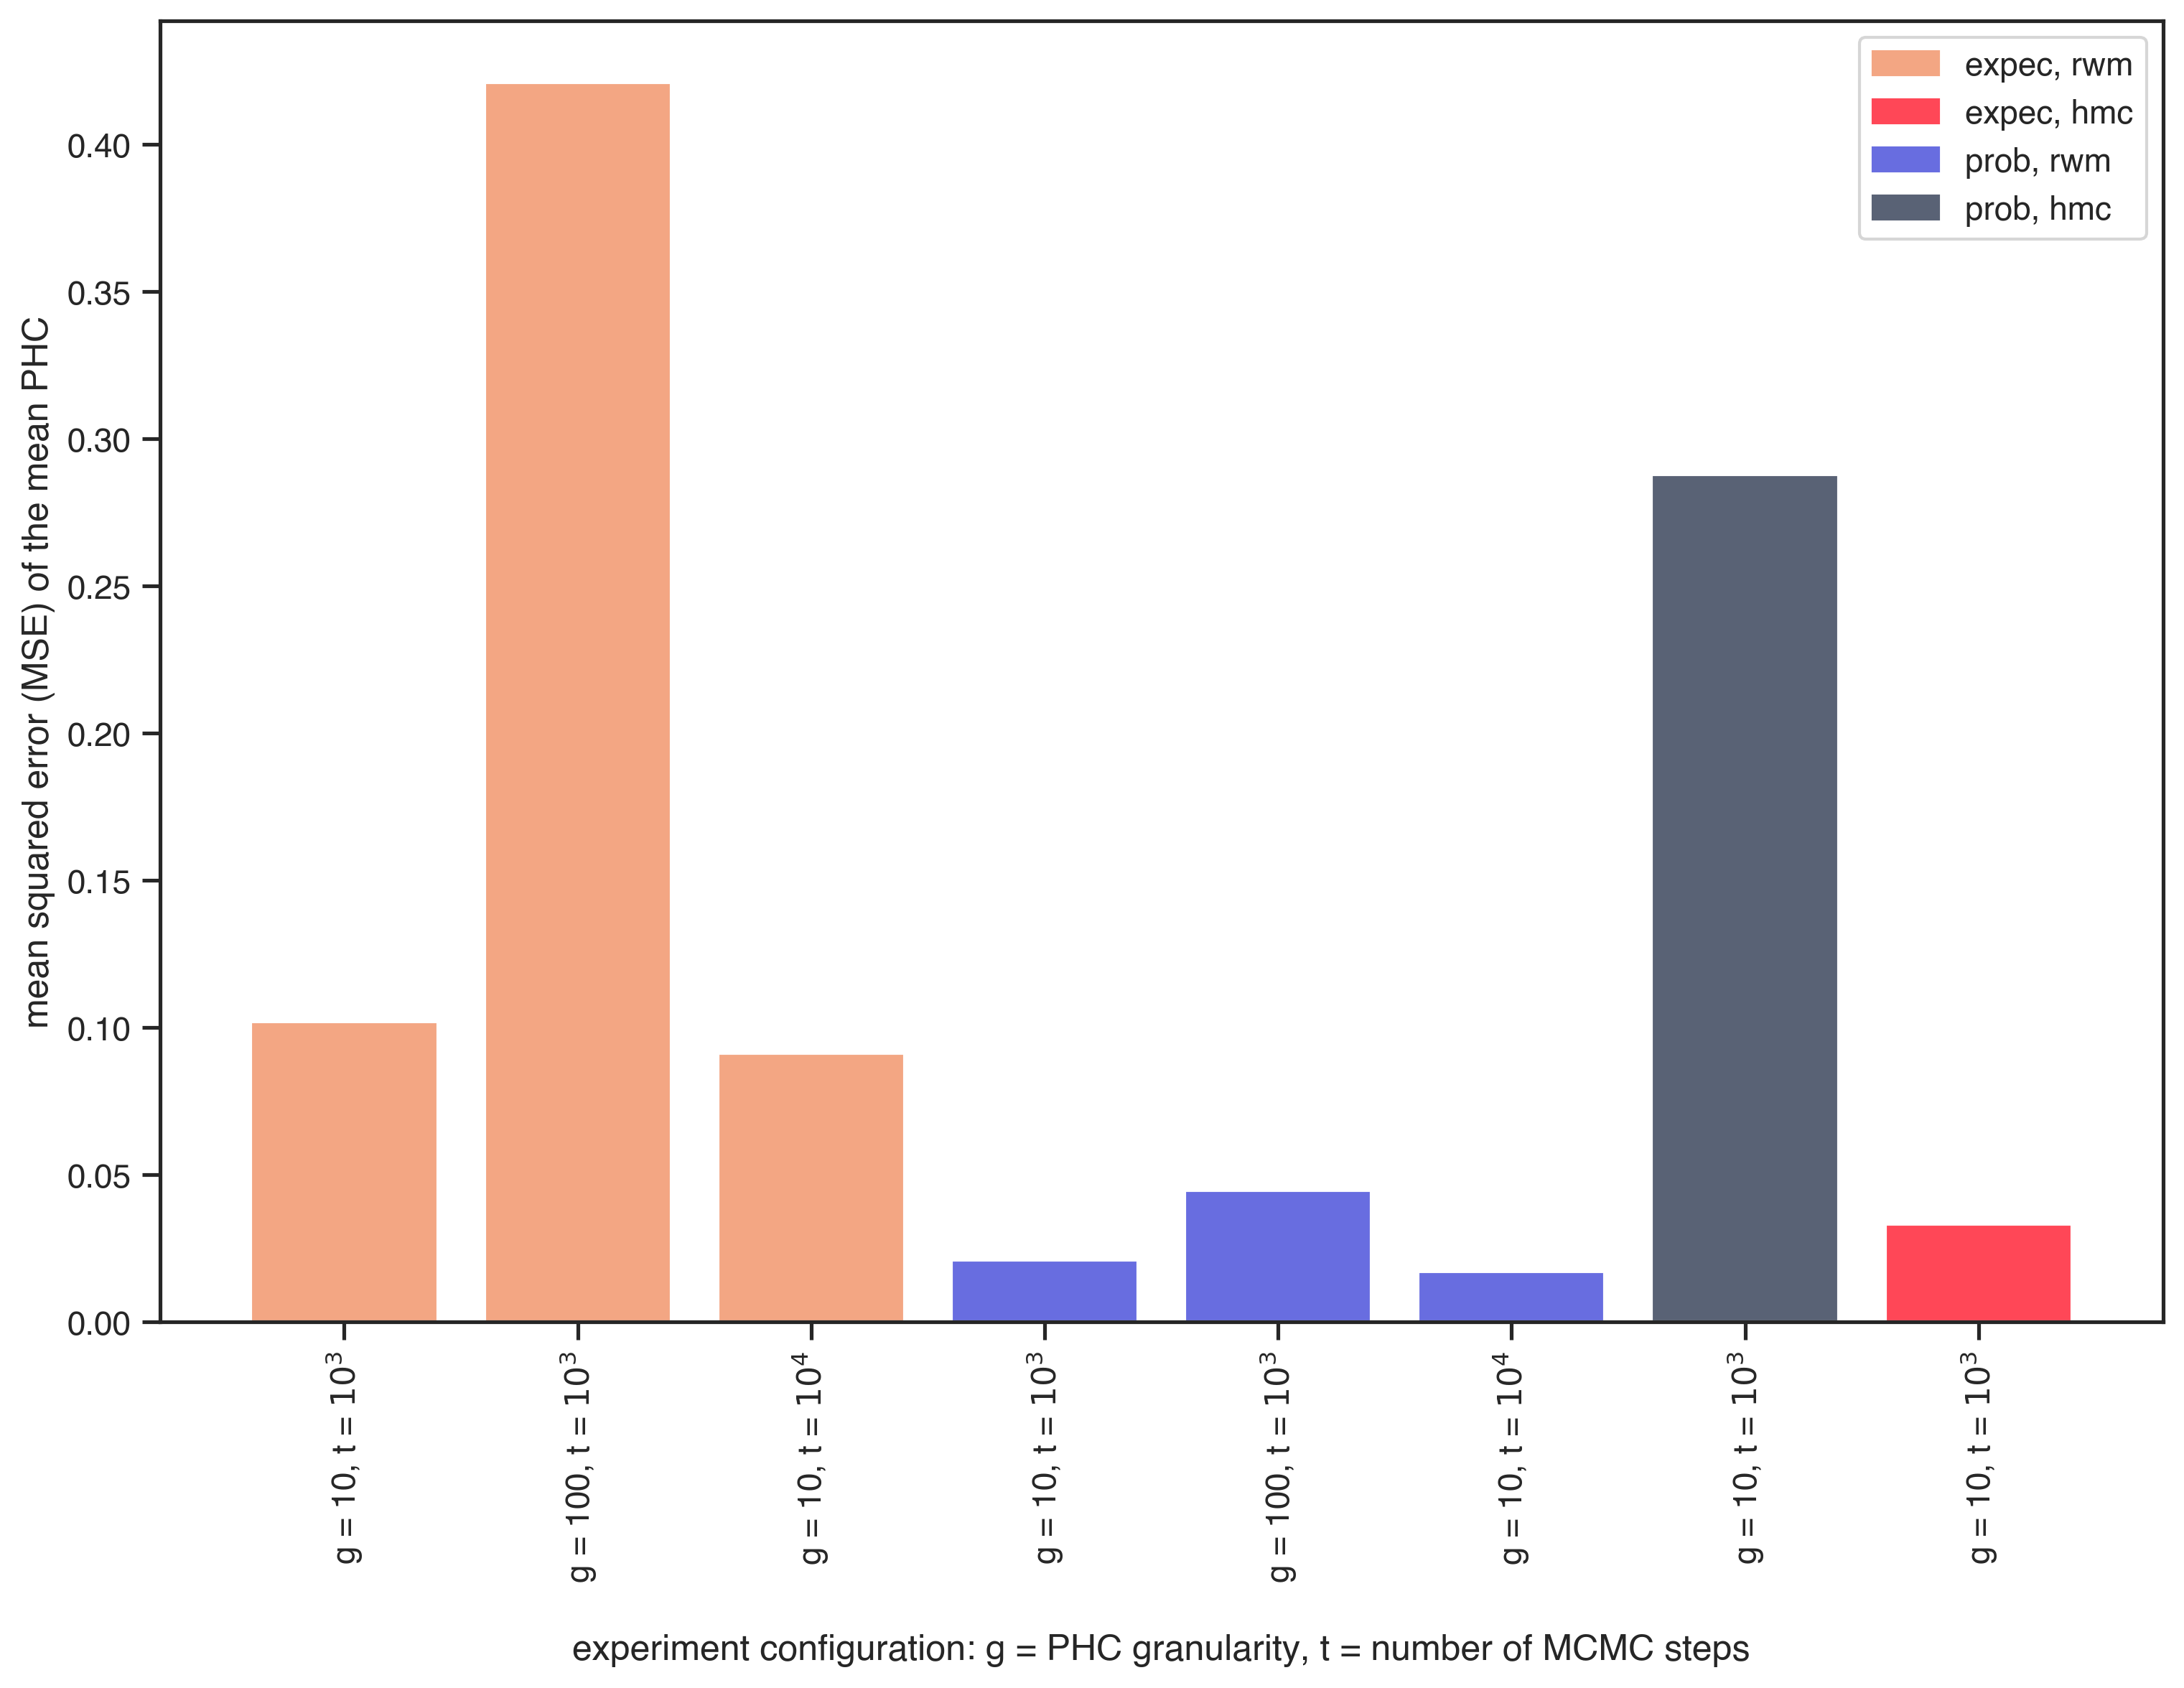
\includegraphics[width=0.75\linewidth]{figures/2_2_mean_mse.png}
 \caption{MSE of the Mean PHC of the Configurations' DVM on the $d_2 \times v_2$ Election}
 \label{fig:2_2_mean_mse}
\end{figure}

\begin{figure}[ht]\centering
 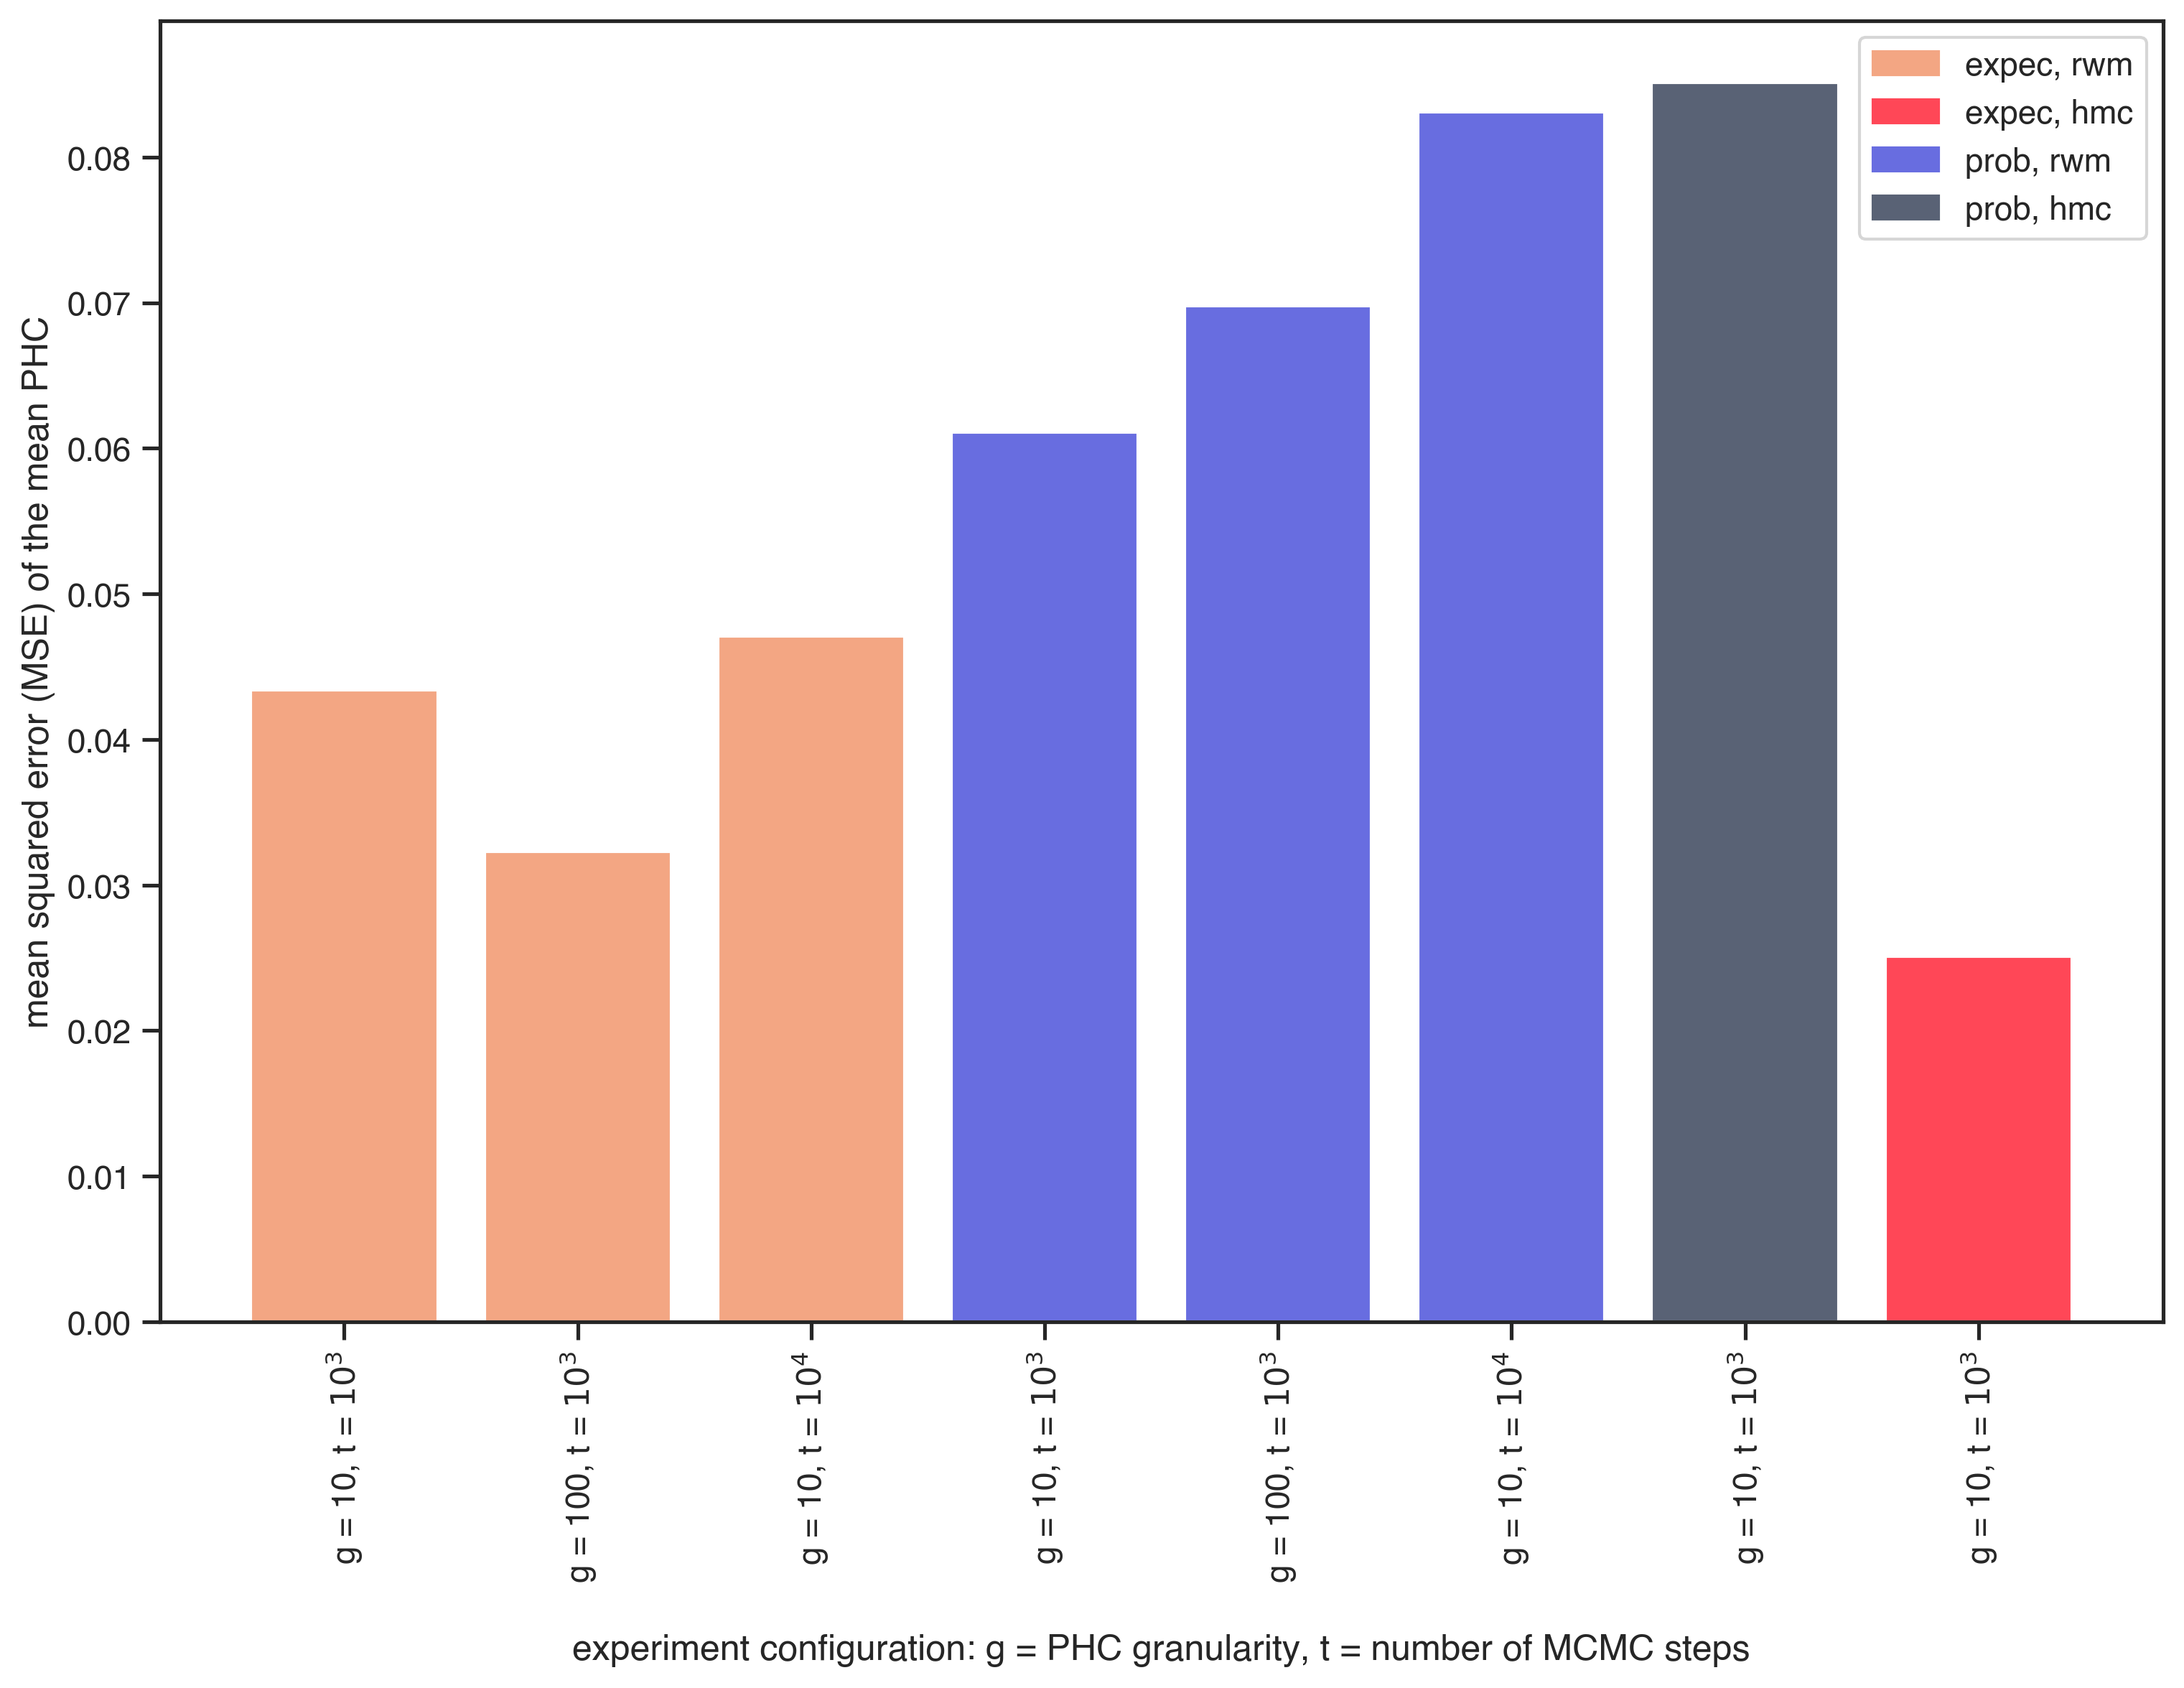
\includegraphics[width=0.75\linewidth]{figures/3_1_mean_mse.png}
 \caption{MSE of the Mean PHC of the Configurations' DVM on the $d_3 \times v_1$ Election}
 \label{fig:3_1_mean_mse}
\end{figure}

\begin{figure}[ht]\centering
 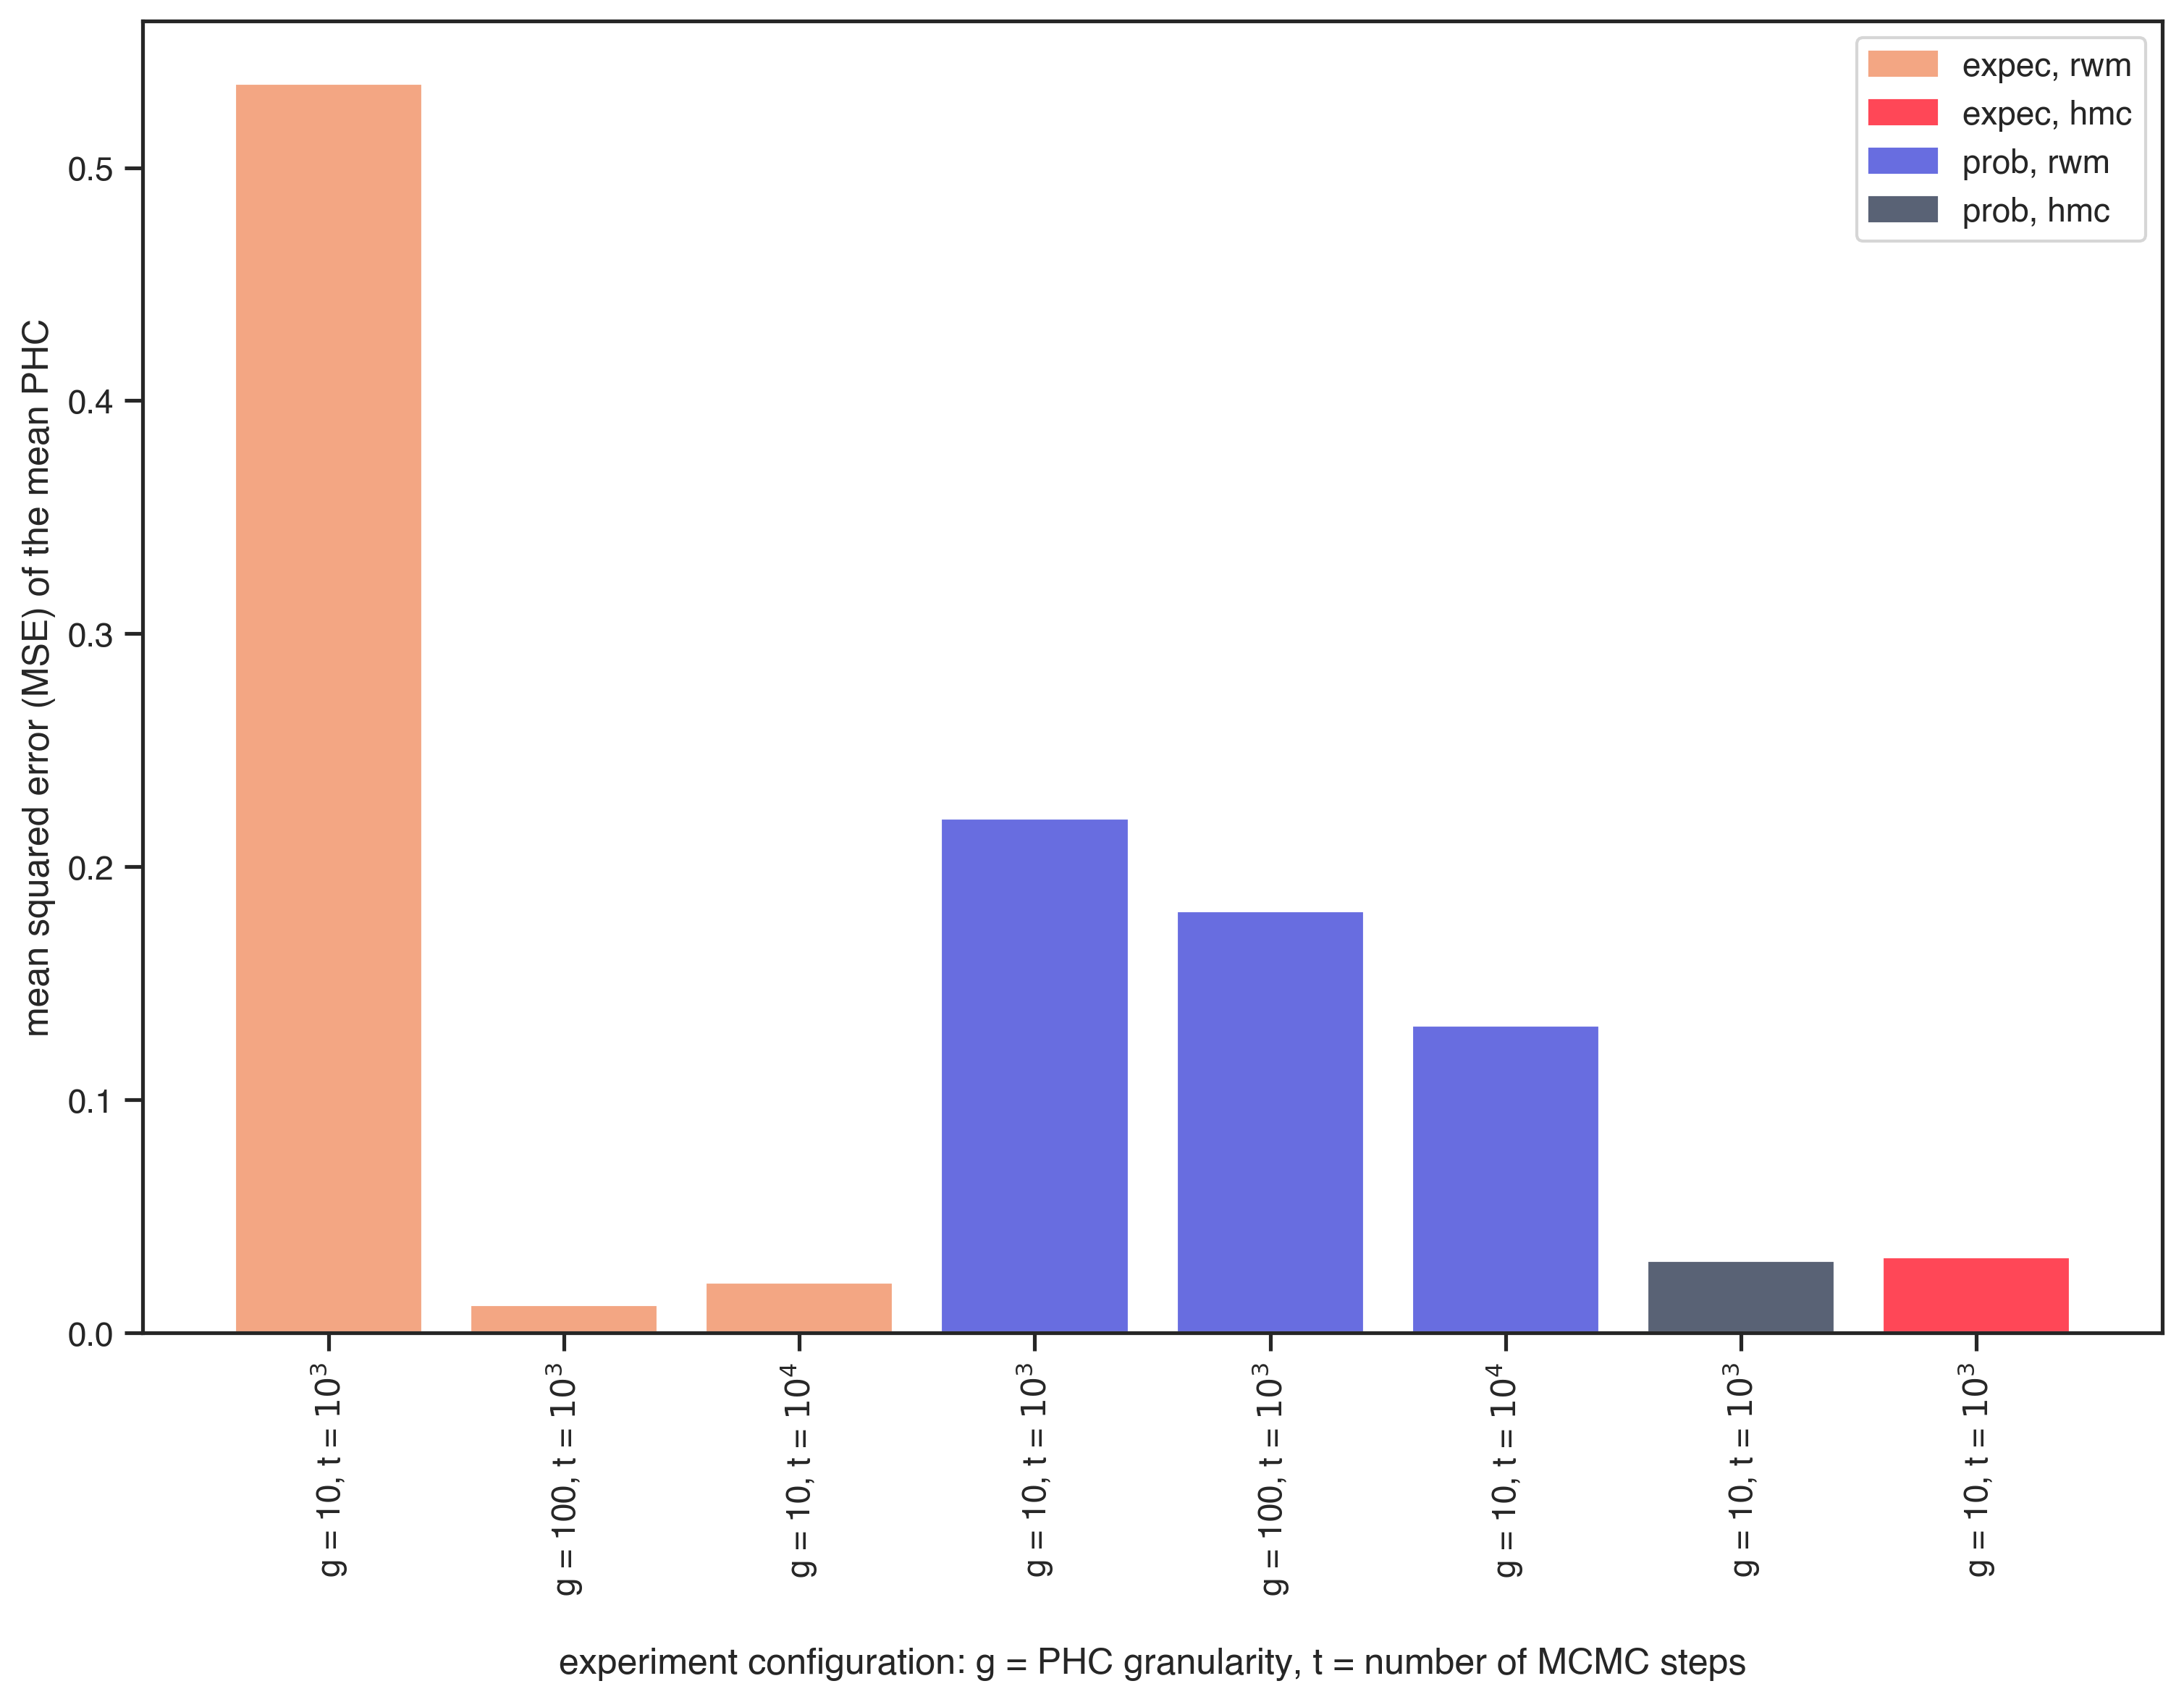
\includegraphics[width=0.75\linewidth]{figures/3_2_mean_mse.png}
 \caption{MSE of the Mean PHC of the Configurations' DVM on the $d_3 \times v_2$ Election}
 \label{fig:3_2_mean_mse}
\end{figure}

\FloatBarrier
\subsection{Runtime of $3 \times 2$ Cases}

\begin{figure}[ht]\centering
 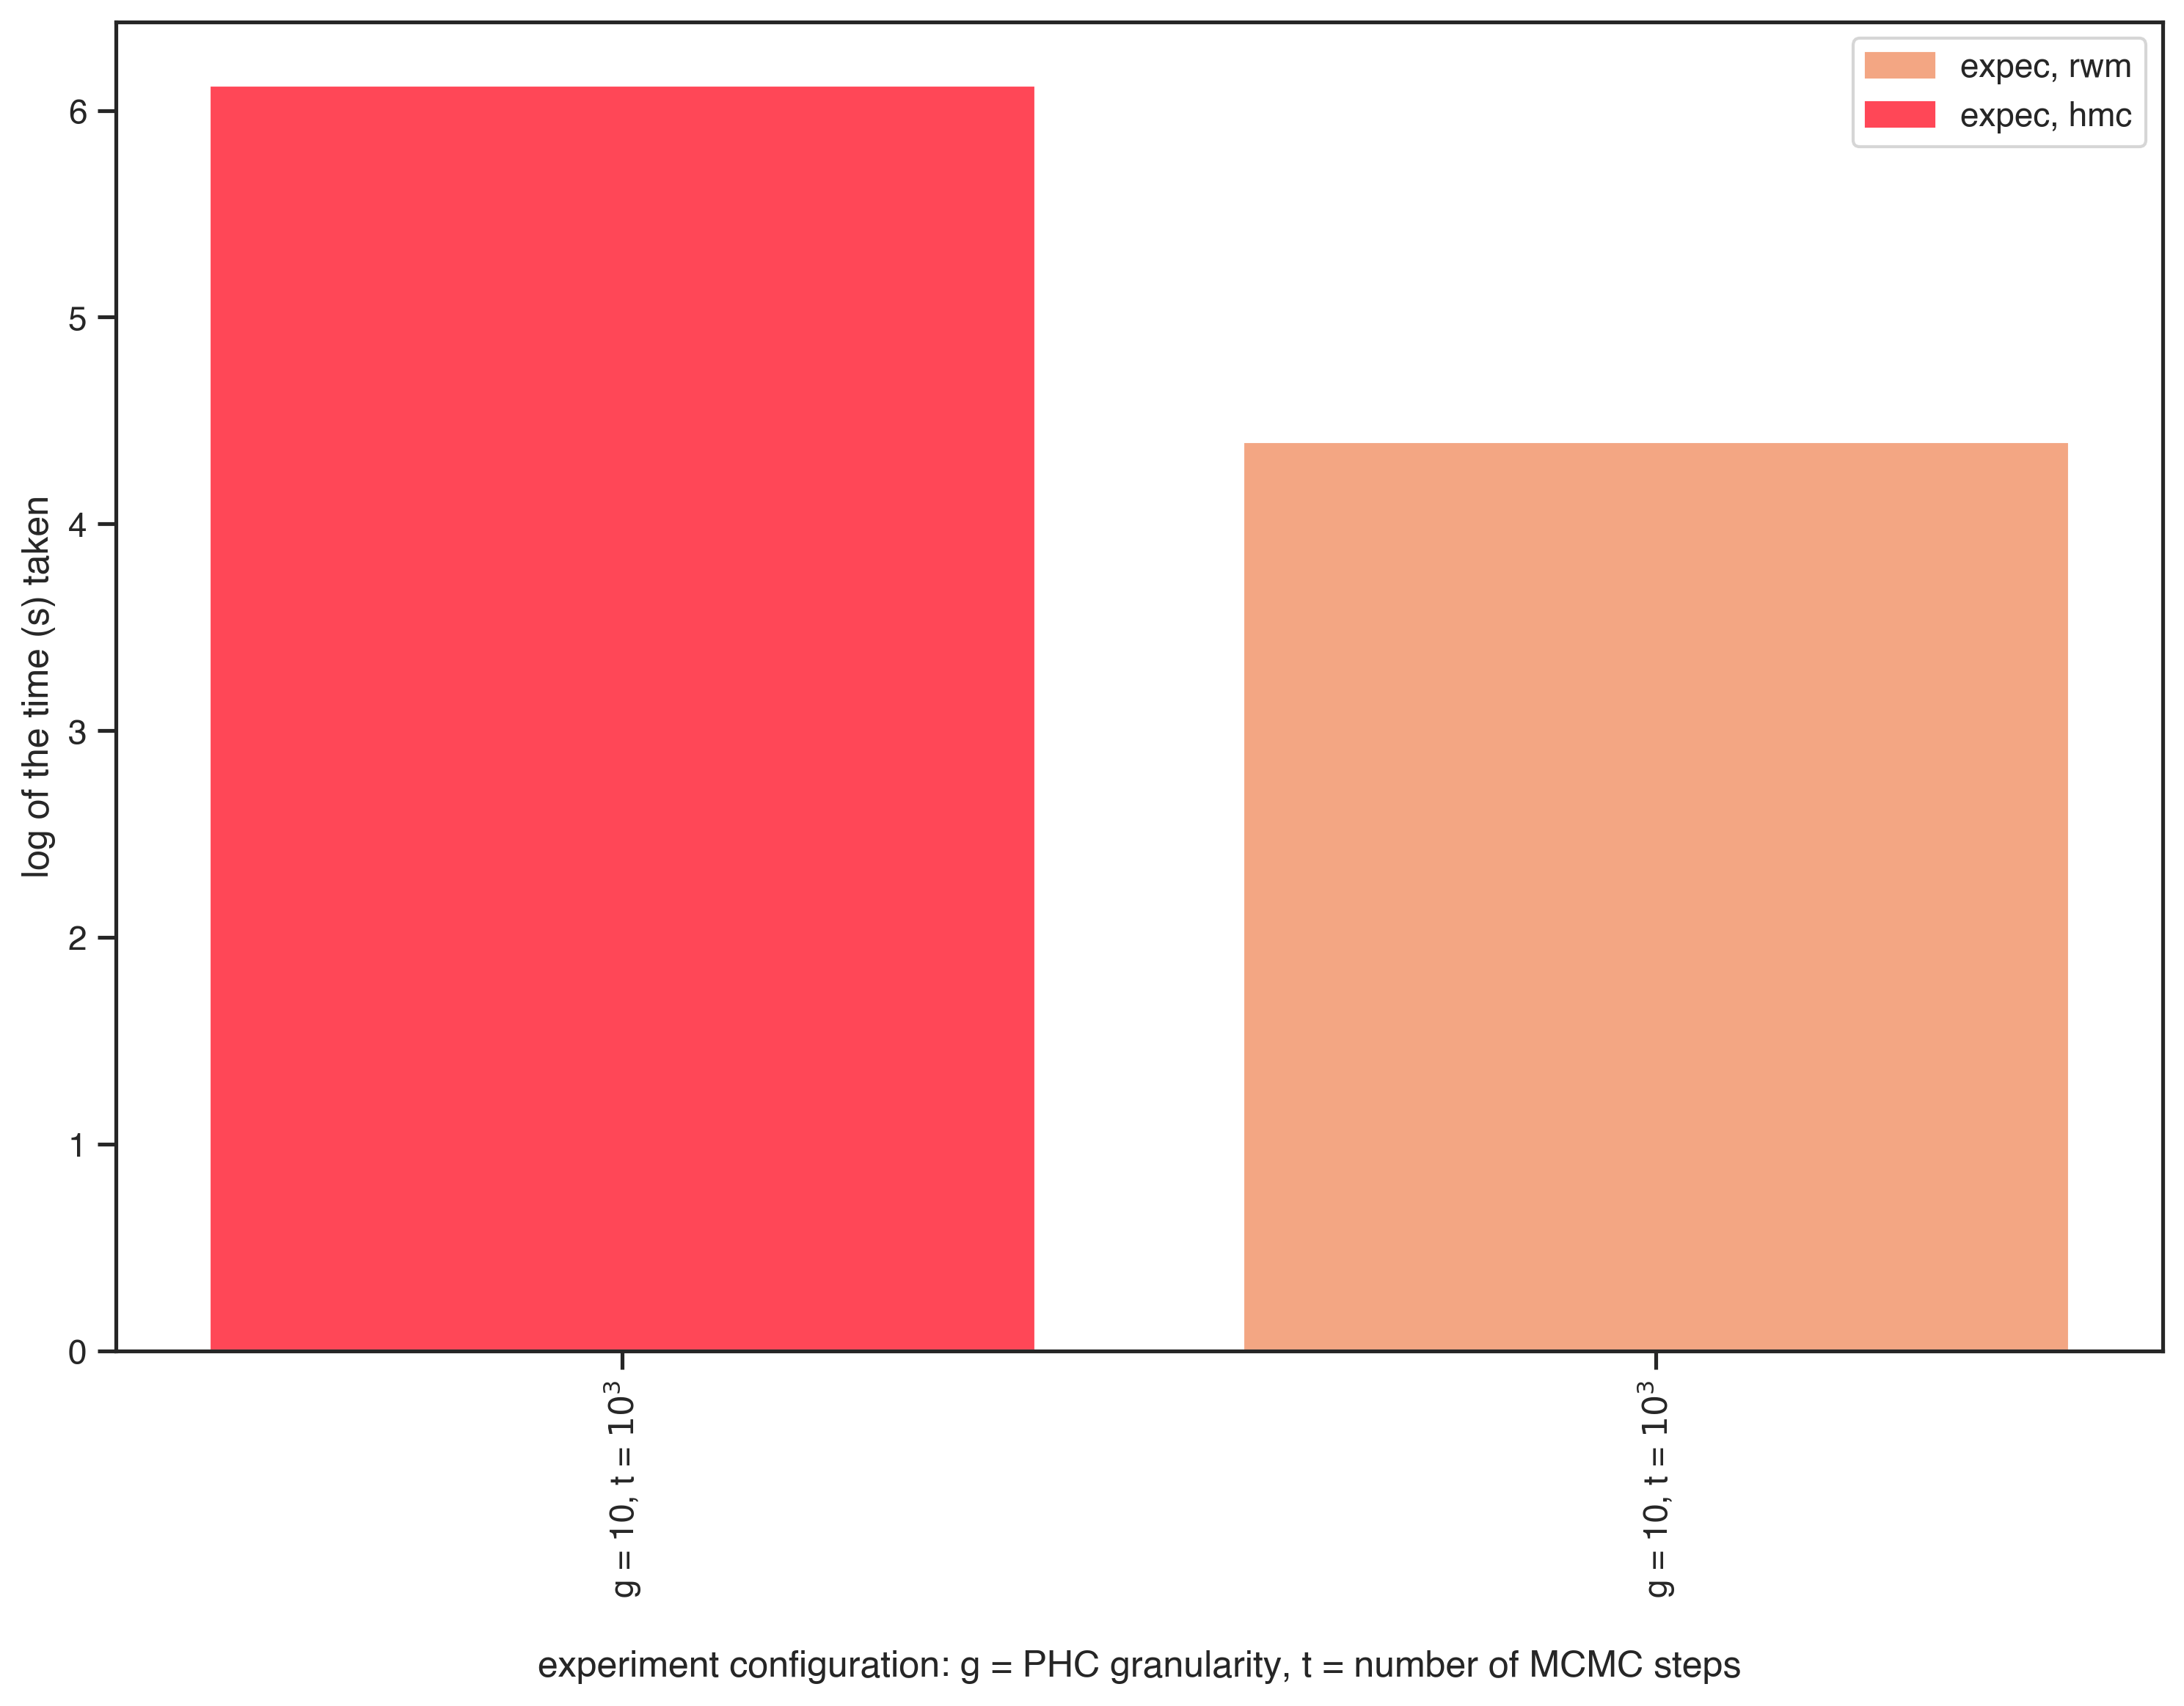
\includegraphics[width=0.75\linewidth]{figures/4_3_time.png}
 \caption{Runtime of the Configurations on the $d_4 \times v_3$ Election}
 \label{fig:4_3_time}
\end{figure}

\begin{figure}[ht]\centering
 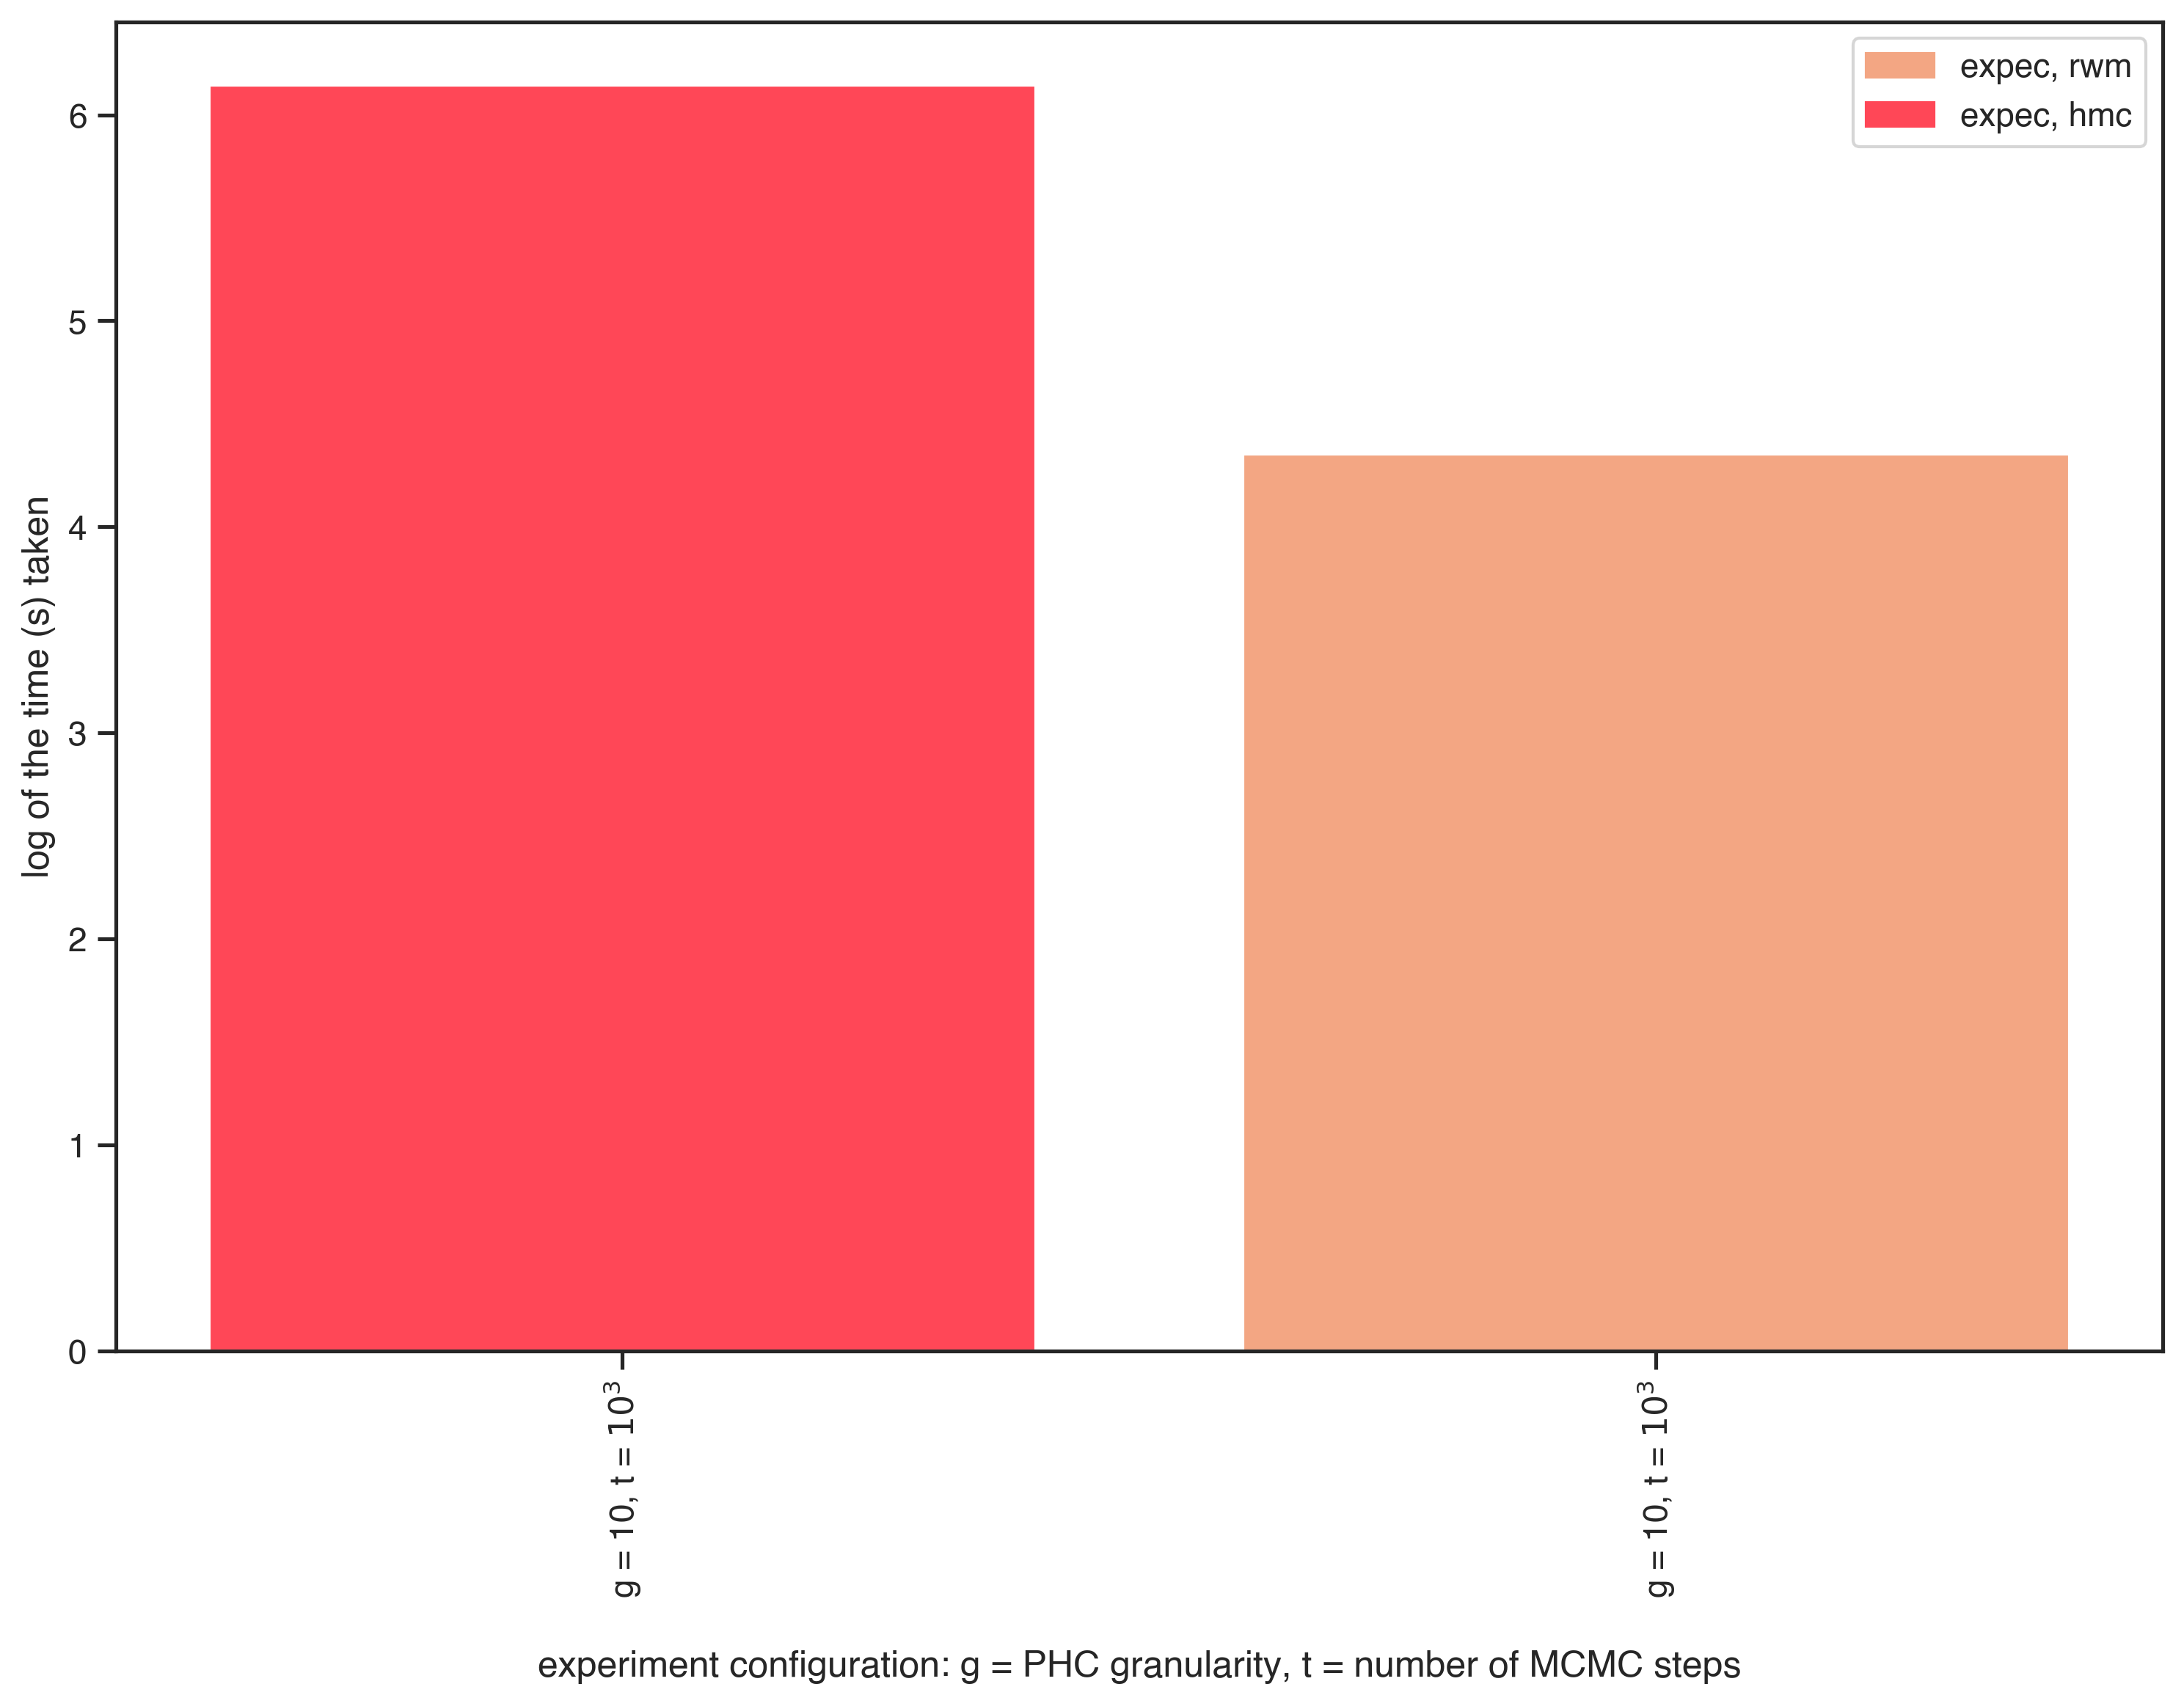
\includegraphics[width=0.75\linewidth]{figures/4_4_time.png}
 \caption{Runtime of the Configurations on the $d_4 \times v_4$ Election}
 \label{fig:4_4_time_append}
\end{figure}

\begin{figure}[ht]\centering
 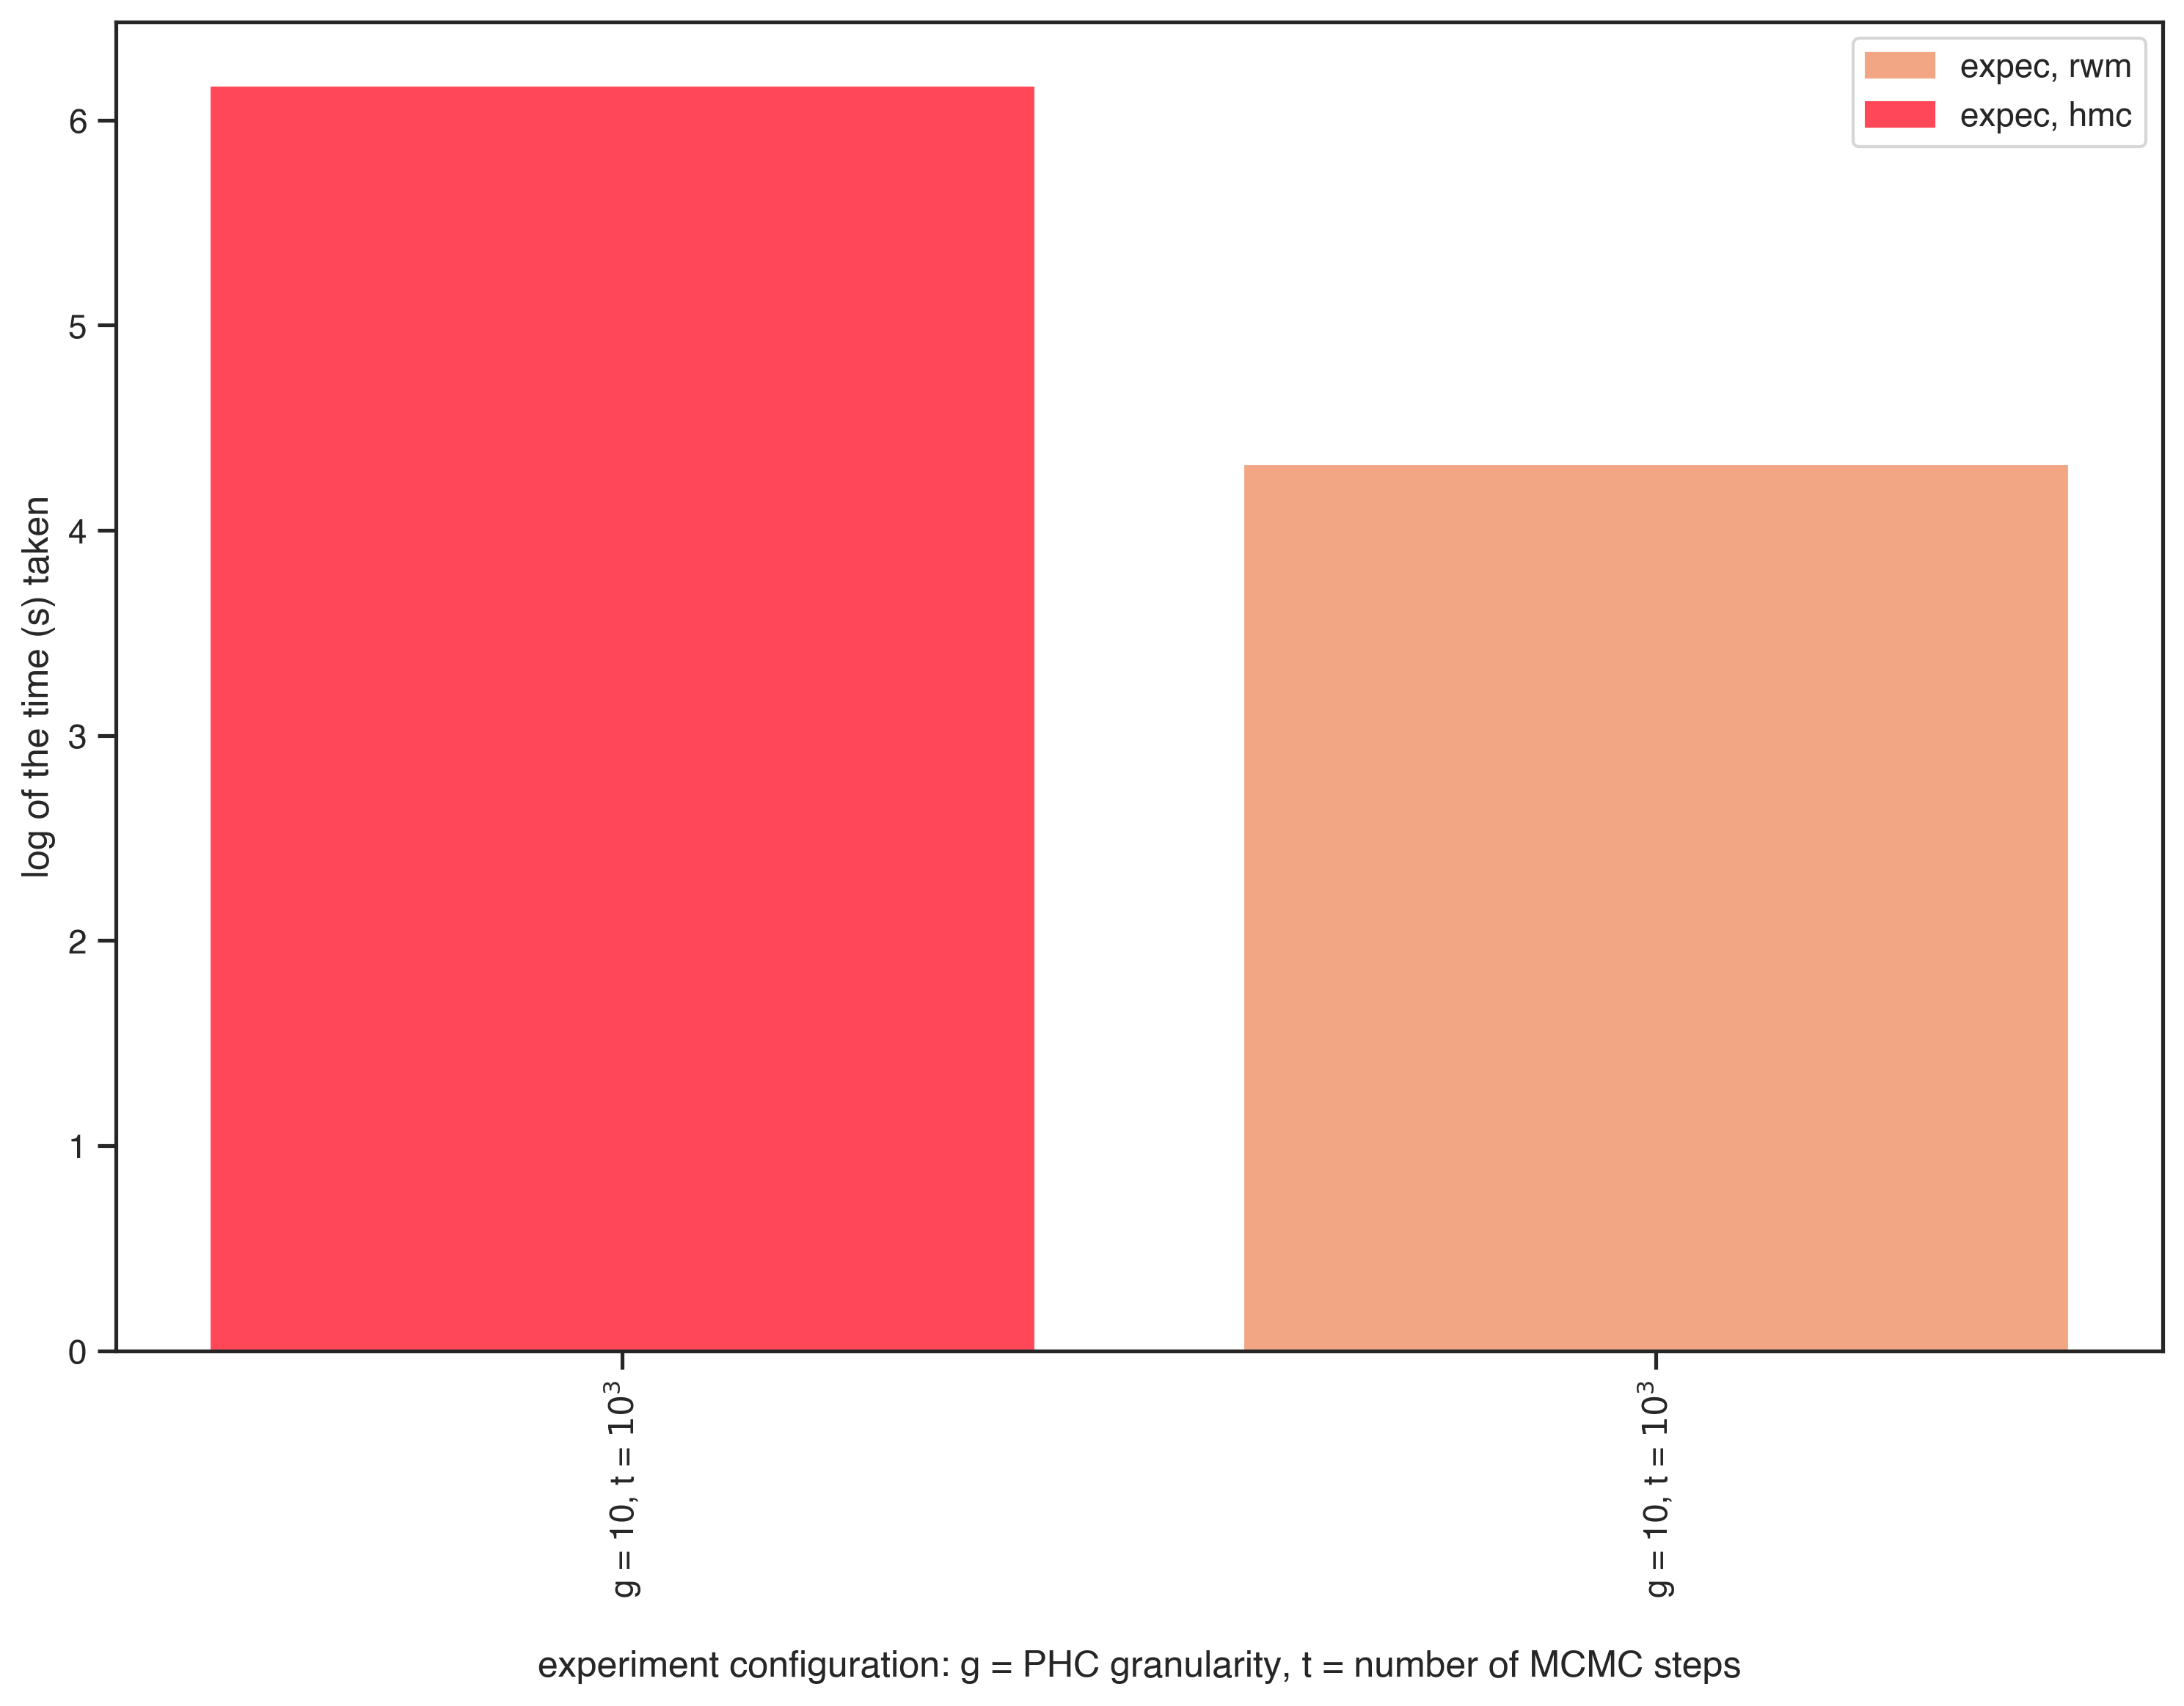
\includegraphics[width=0.75\linewidth]{figures/5_3_time.png}
 \caption{Runtime of the Configurations on the $d_5 \times v_3$ Election}
 \label{fig:5_3_time}
\end{figure}

\begin{figure}[ht]\centering
 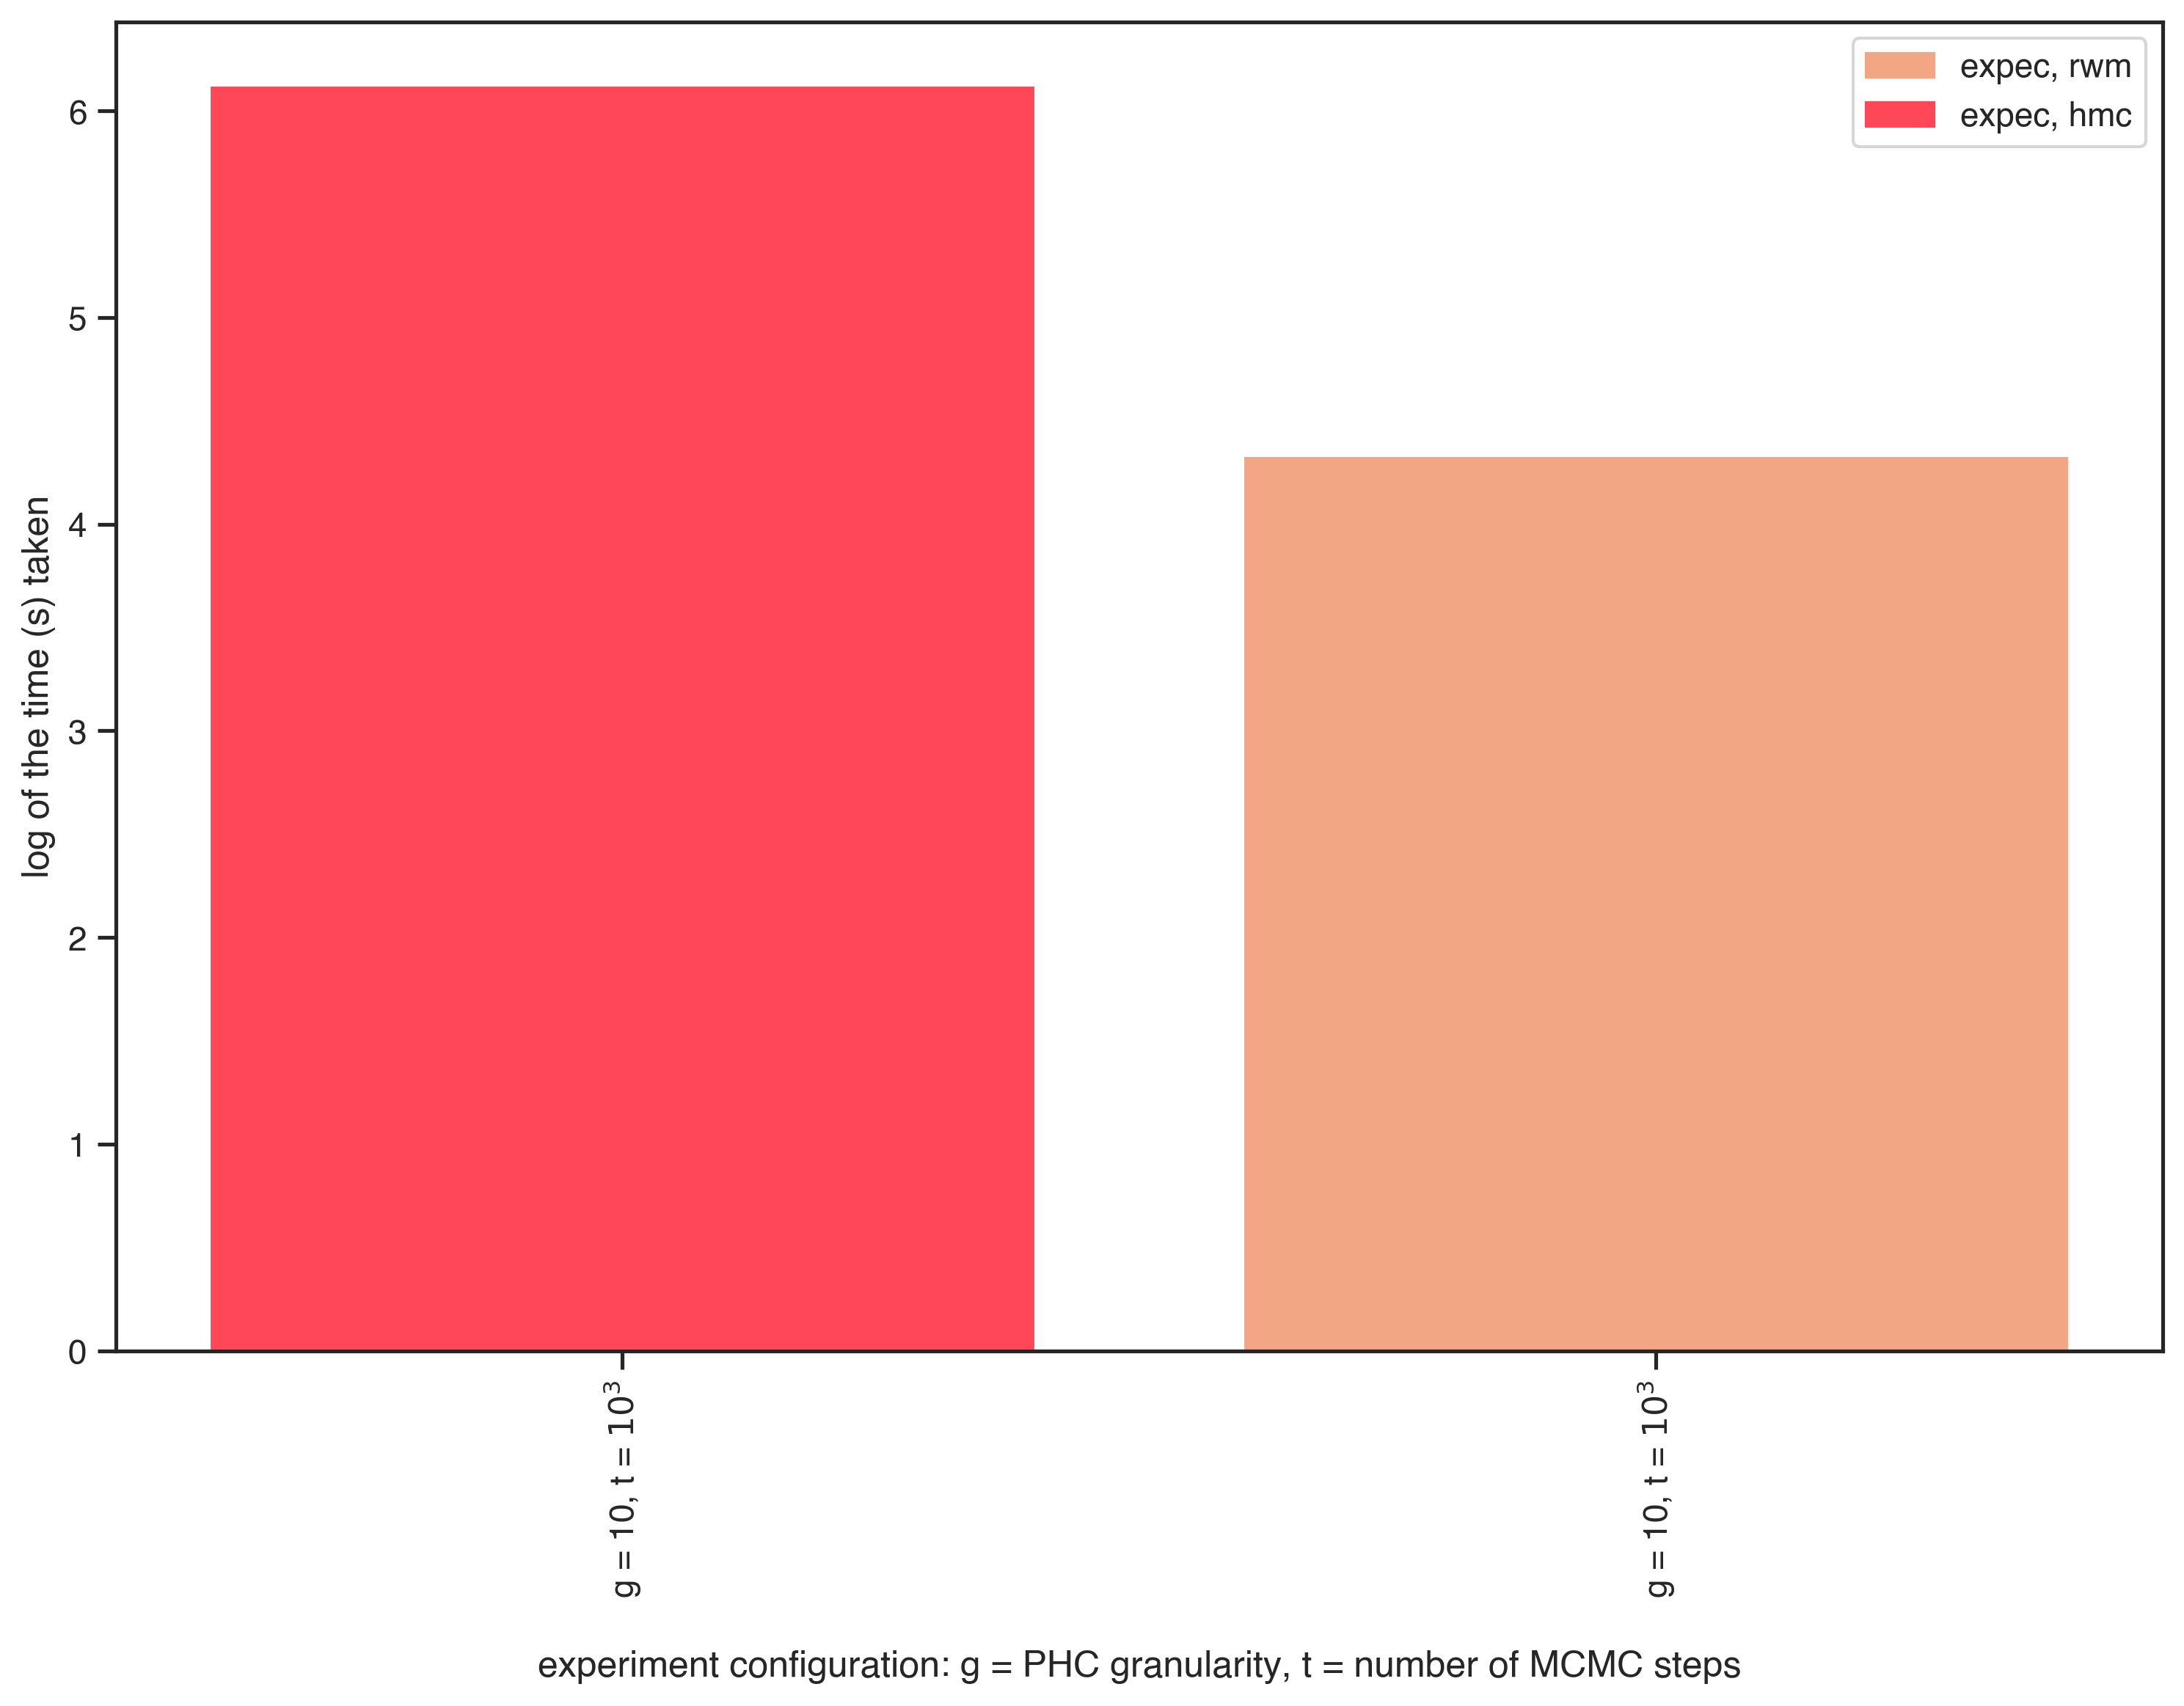
\includegraphics[width=0.75\linewidth]{figures/5_4_time.png}
 \caption{Runtime of the Configurations on the $d_5 \times v_4$ Election}
 \label{fig:5_4_time}
\end{figure}

\begin{figure}[ht]\centering
 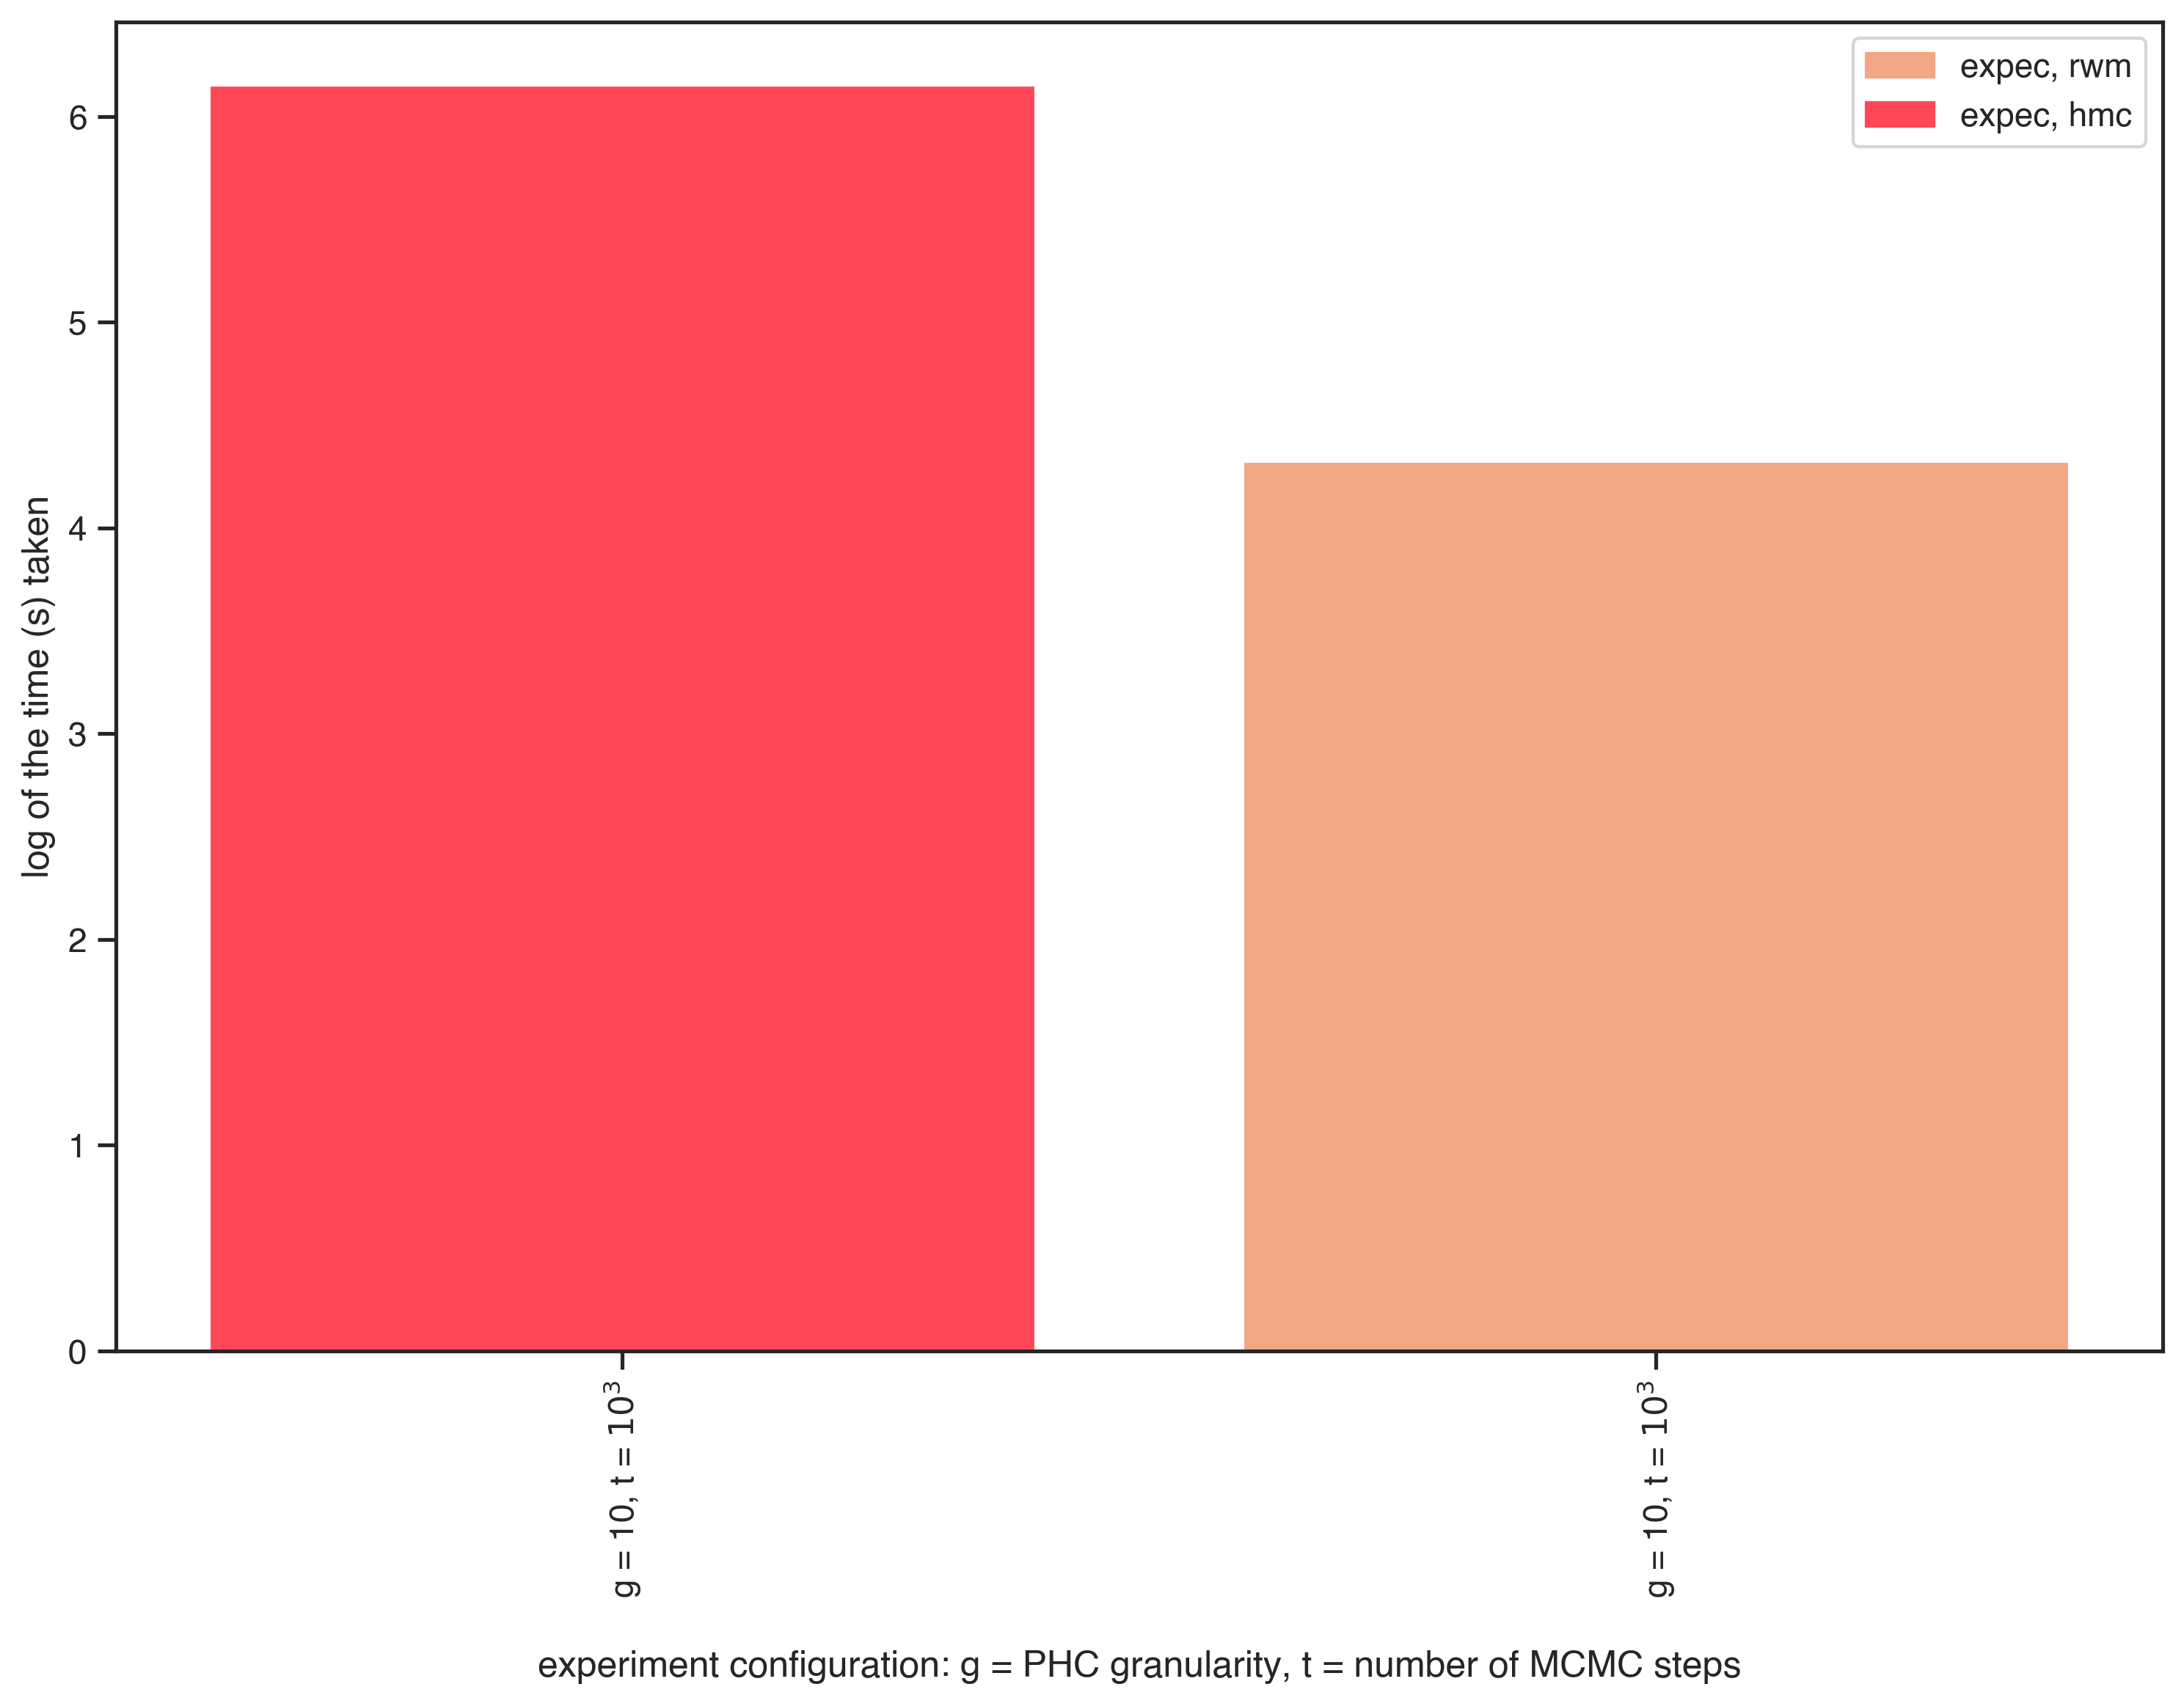
\includegraphics[width=0.75\linewidth]{figures/6_3_time.png}
 \caption{Runtime of the Configurations on the $d_6 \times v_3$ Election}
 \label{fig:6_3_time}
\end{figure}

\begin{figure}[ht]\centering
 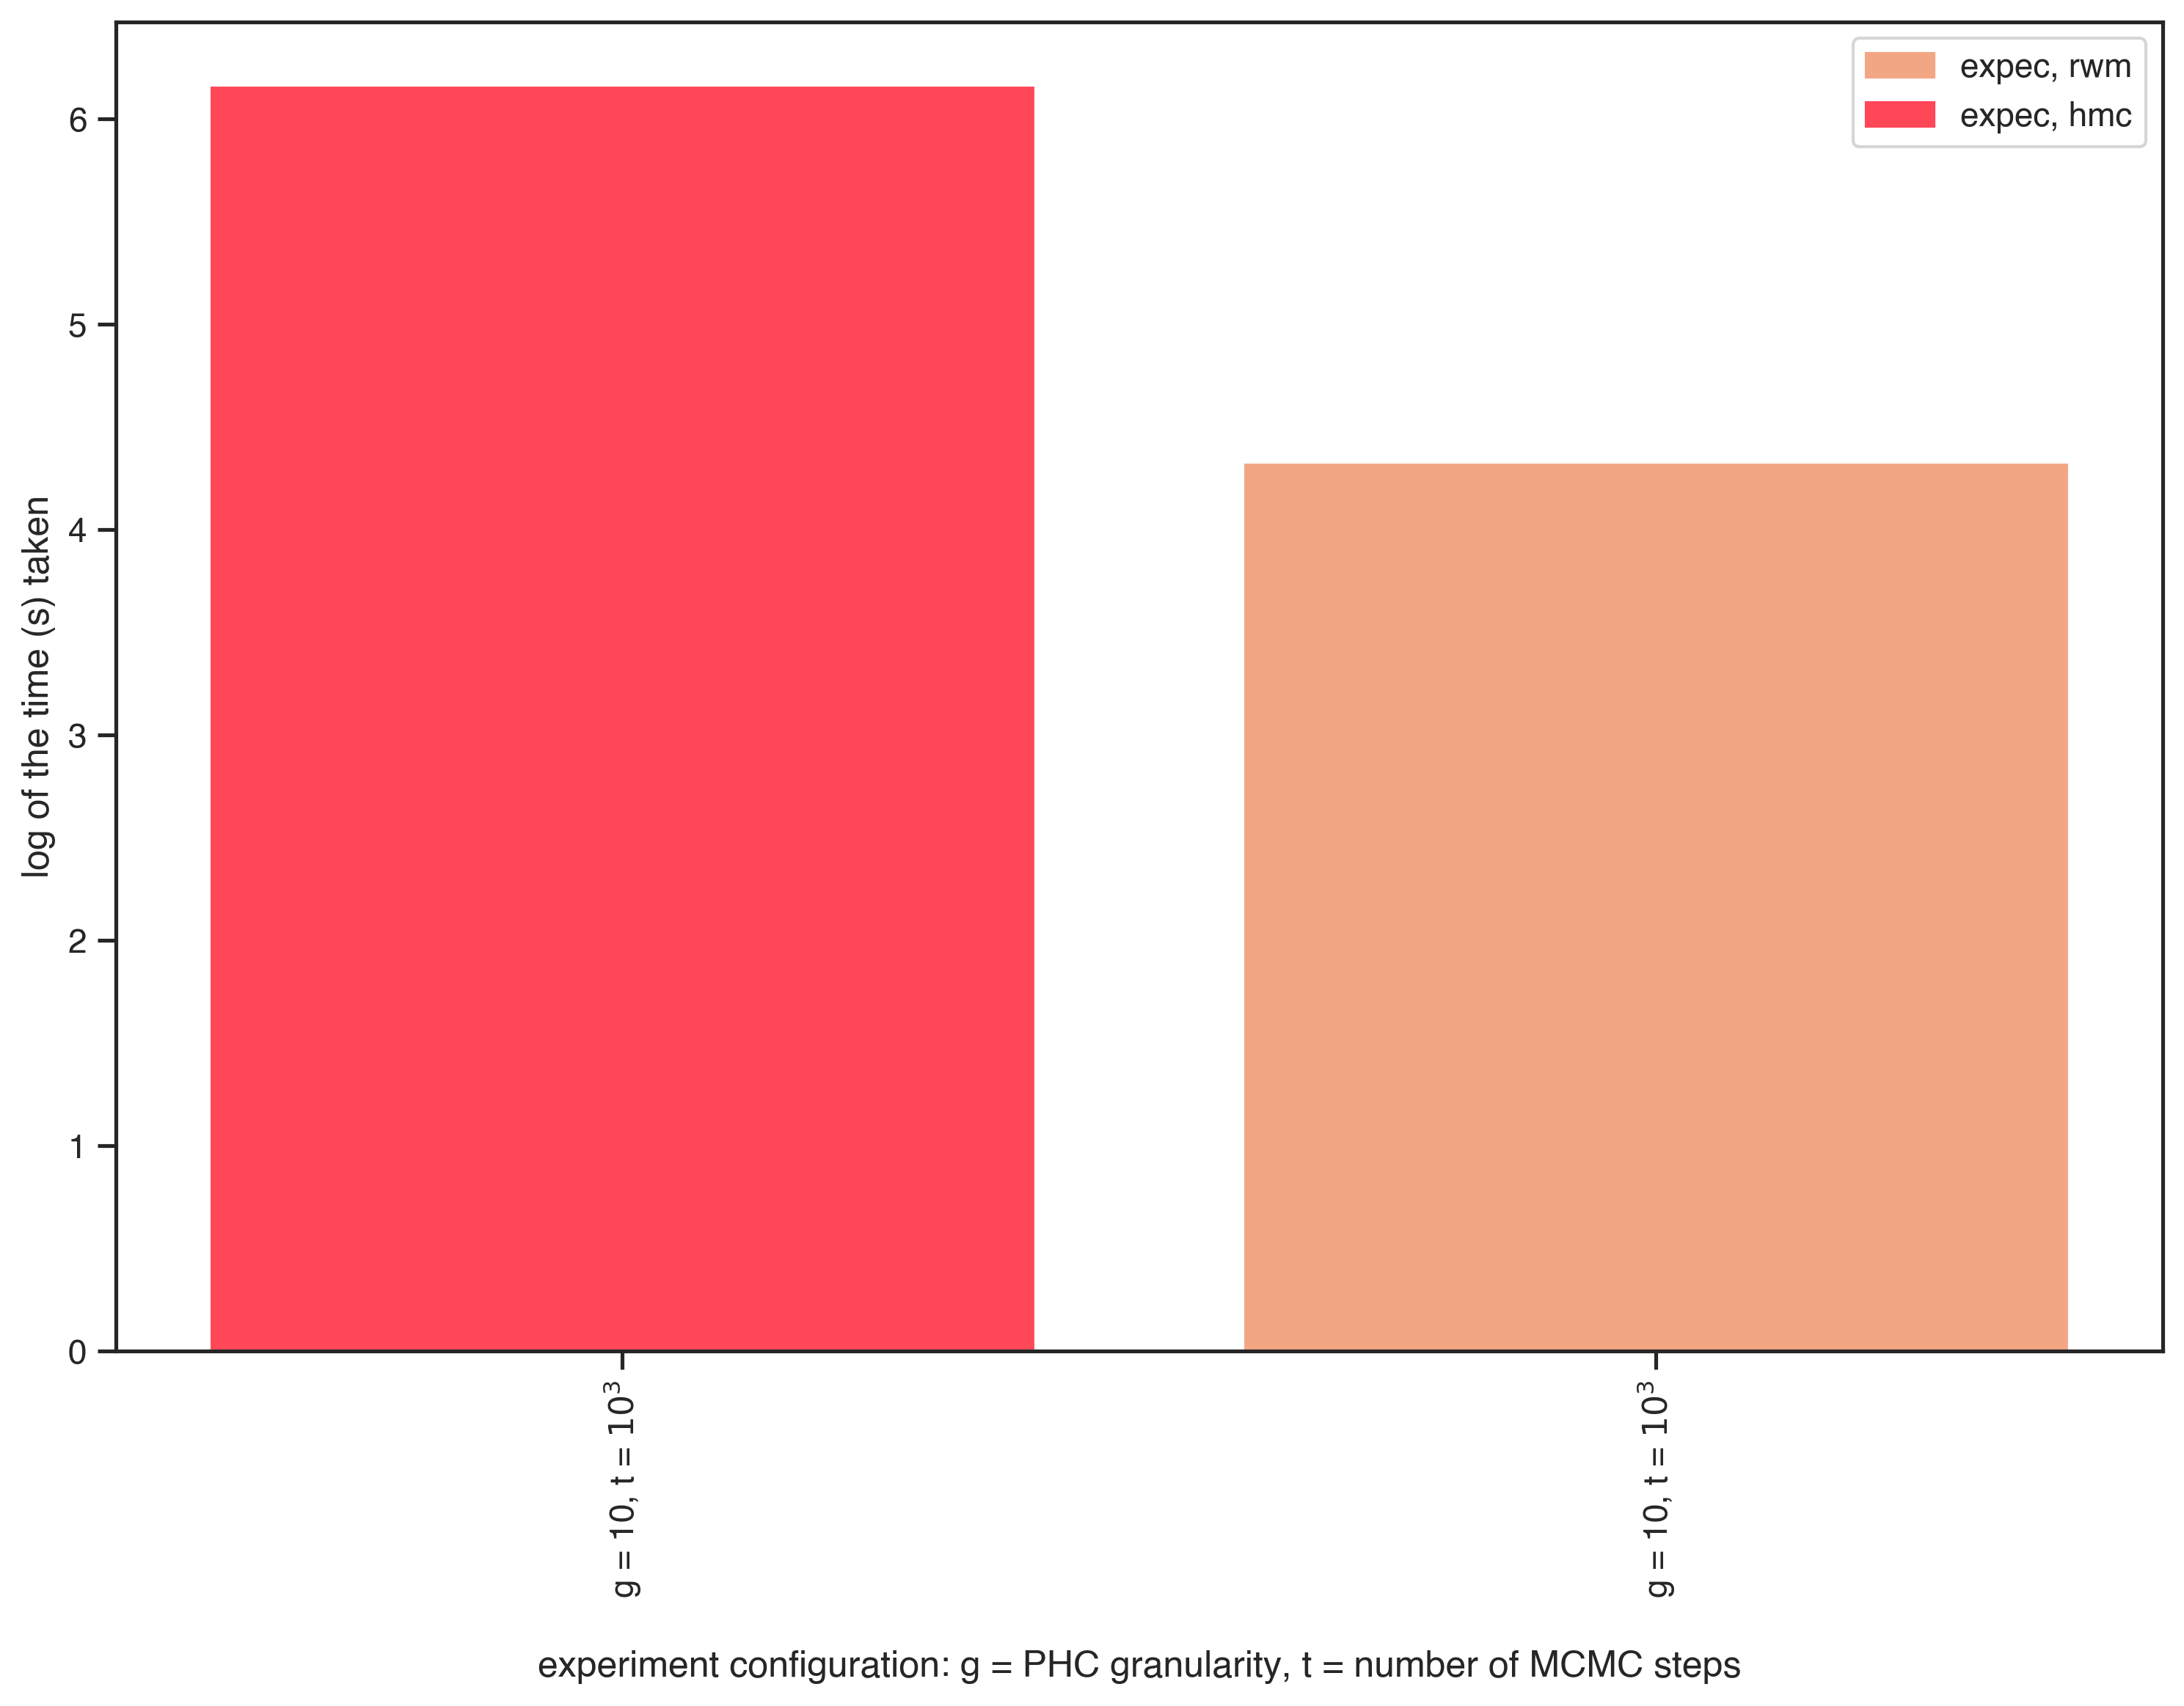
\includegraphics[width=0.75\linewidth]{figures/6_4_time.png}
 \caption{Runtime of the Configurations on the $d_6 \times v_4$ Election}
 \label{fig:6_4_time}
\end{figure}

\FloatBarrier
\subsection{Mean PHC MSE of $3 \times 2$ Cases}

\begin{figure}[ht]\centering
 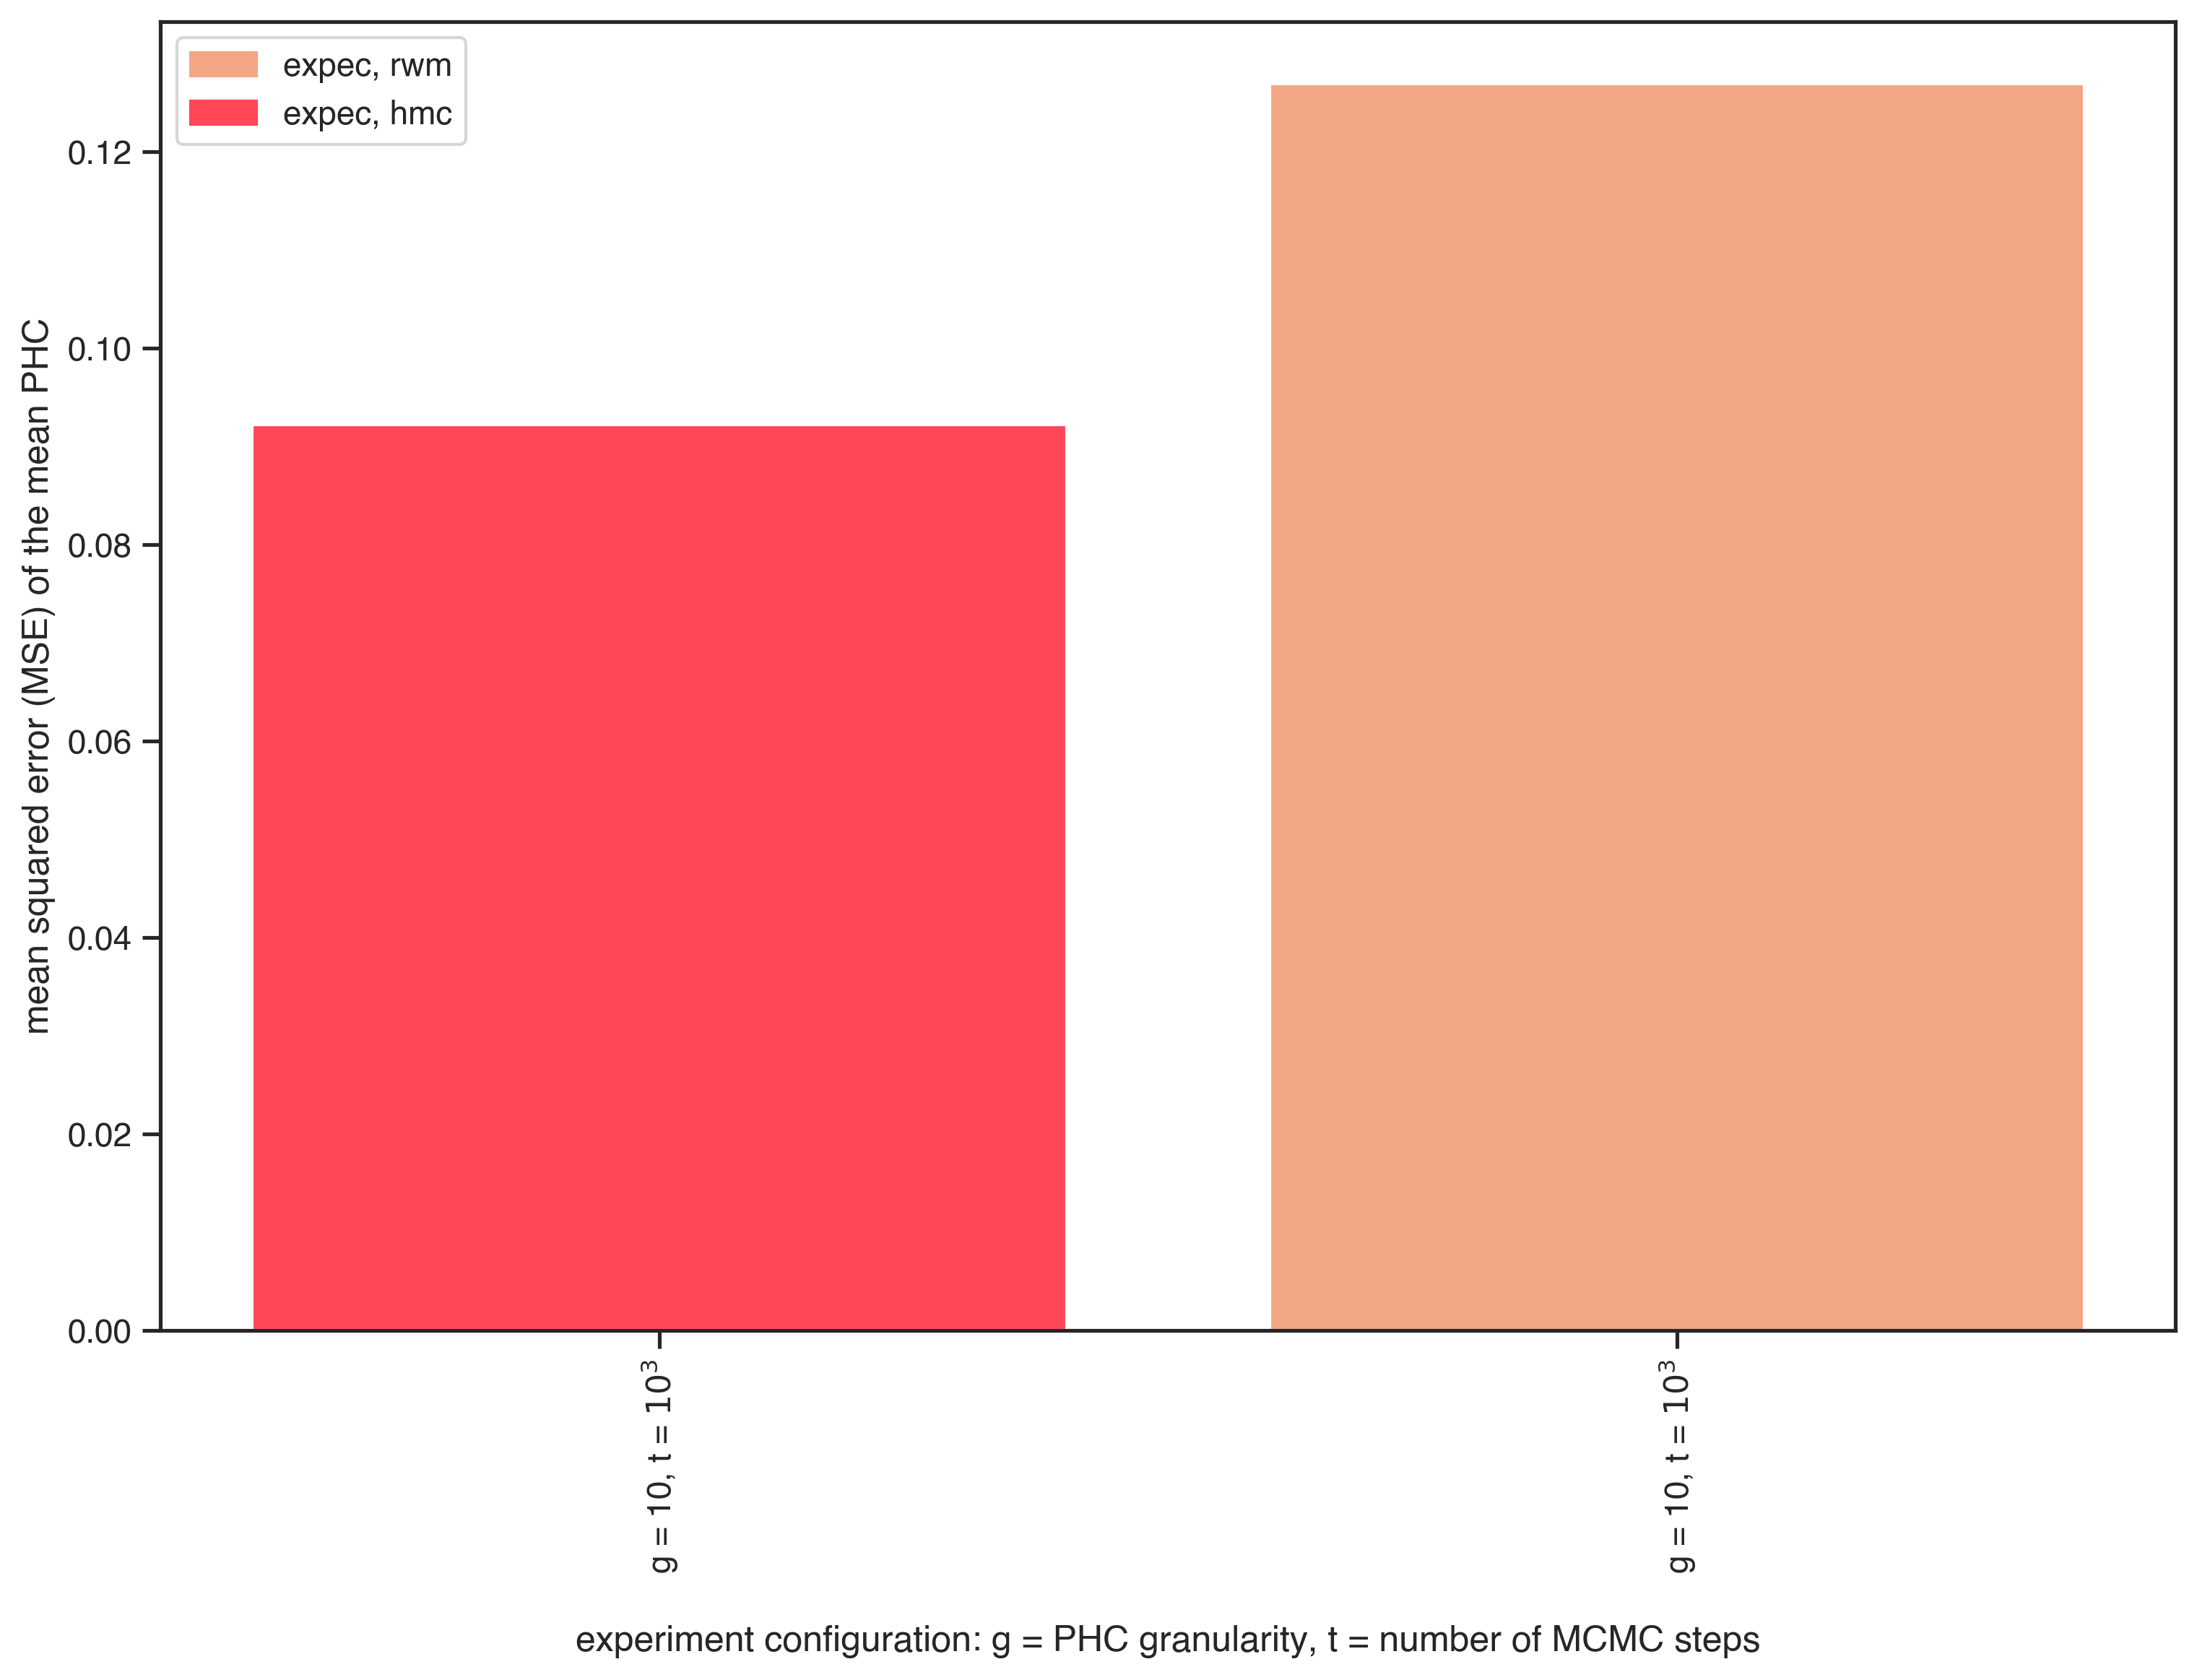
\includegraphics[width=0.75\linewidth]{figures/4_3_mean_mse.png}
 \caption{MSE of the Mean PHC of the Configurations' DVM on the $d_4 \times v_3$ Election}
 \label{fig:4_3_mean_mse}
\end{figure}

\begin{figure}[ht]\centering
 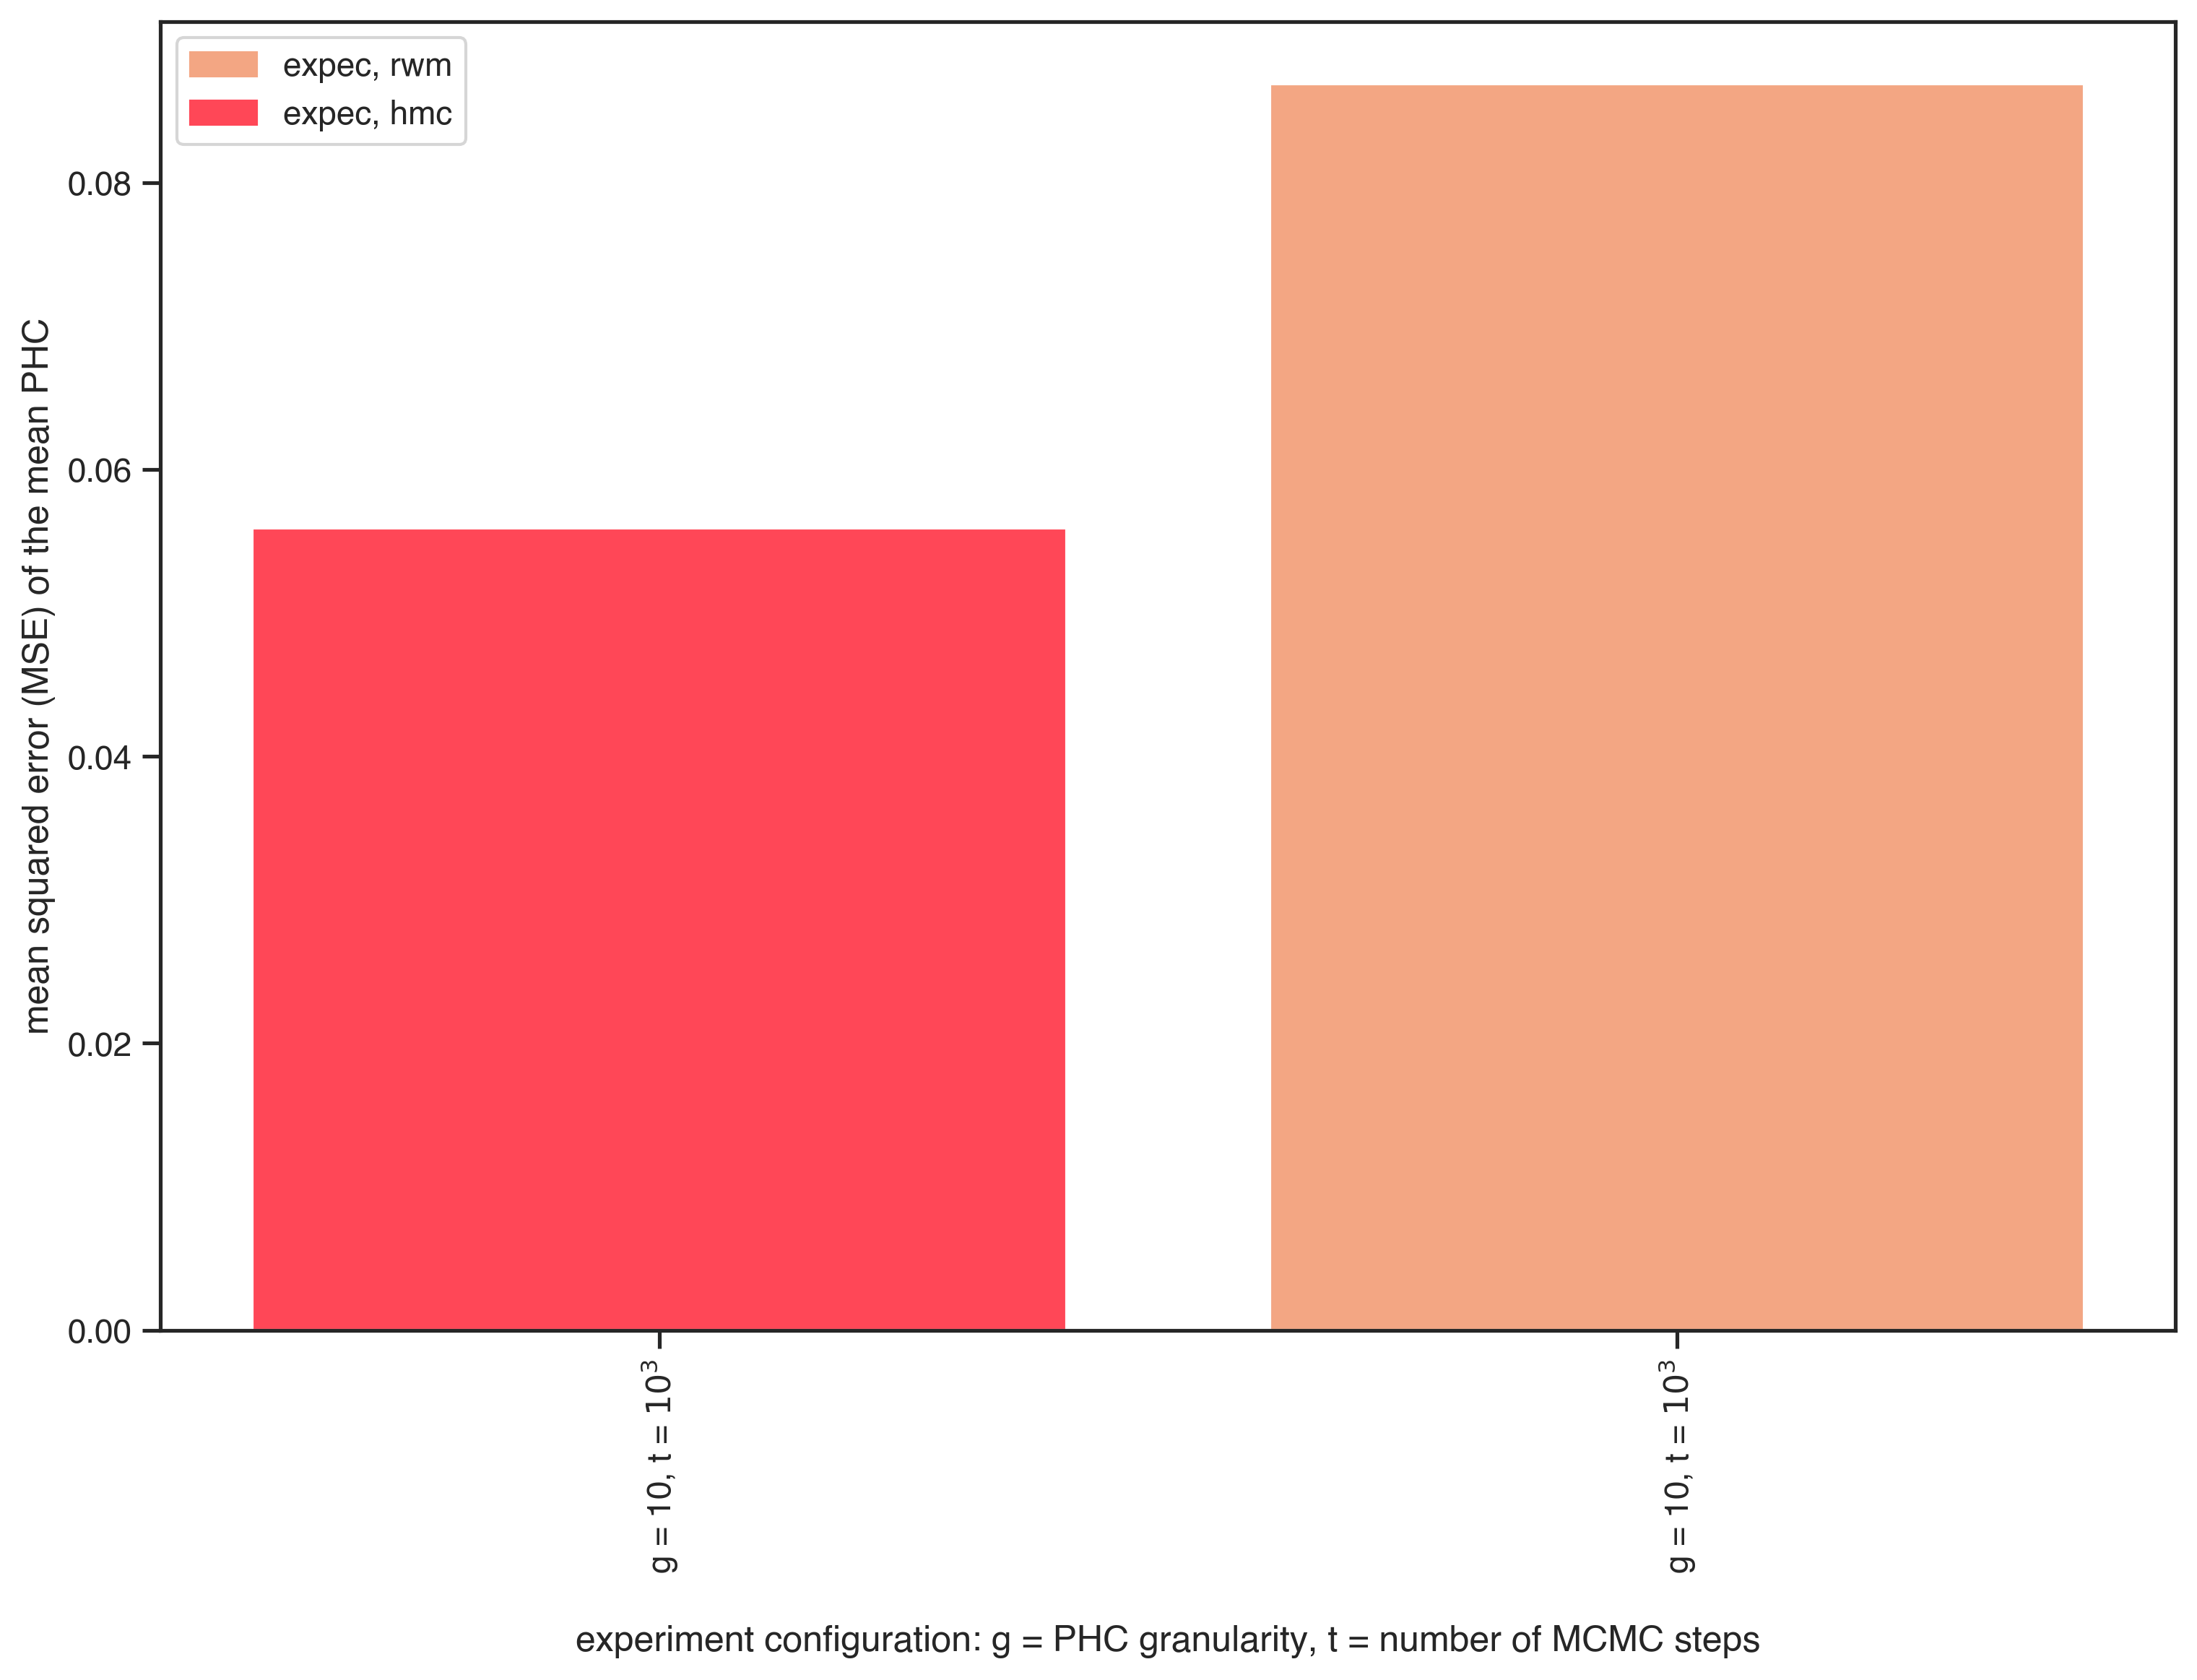
\includegraphics[width=0.75\linewidth]{figures/4_4_mean_mse.png}
 \caption{MSE of the Mean PHC of the Configurations' DVM on the $d_4 \times v_4$ Election}
 \label{fig:4_4_mean_mse_append}
\end{figure}

\begin{figure}[ht]\centering
 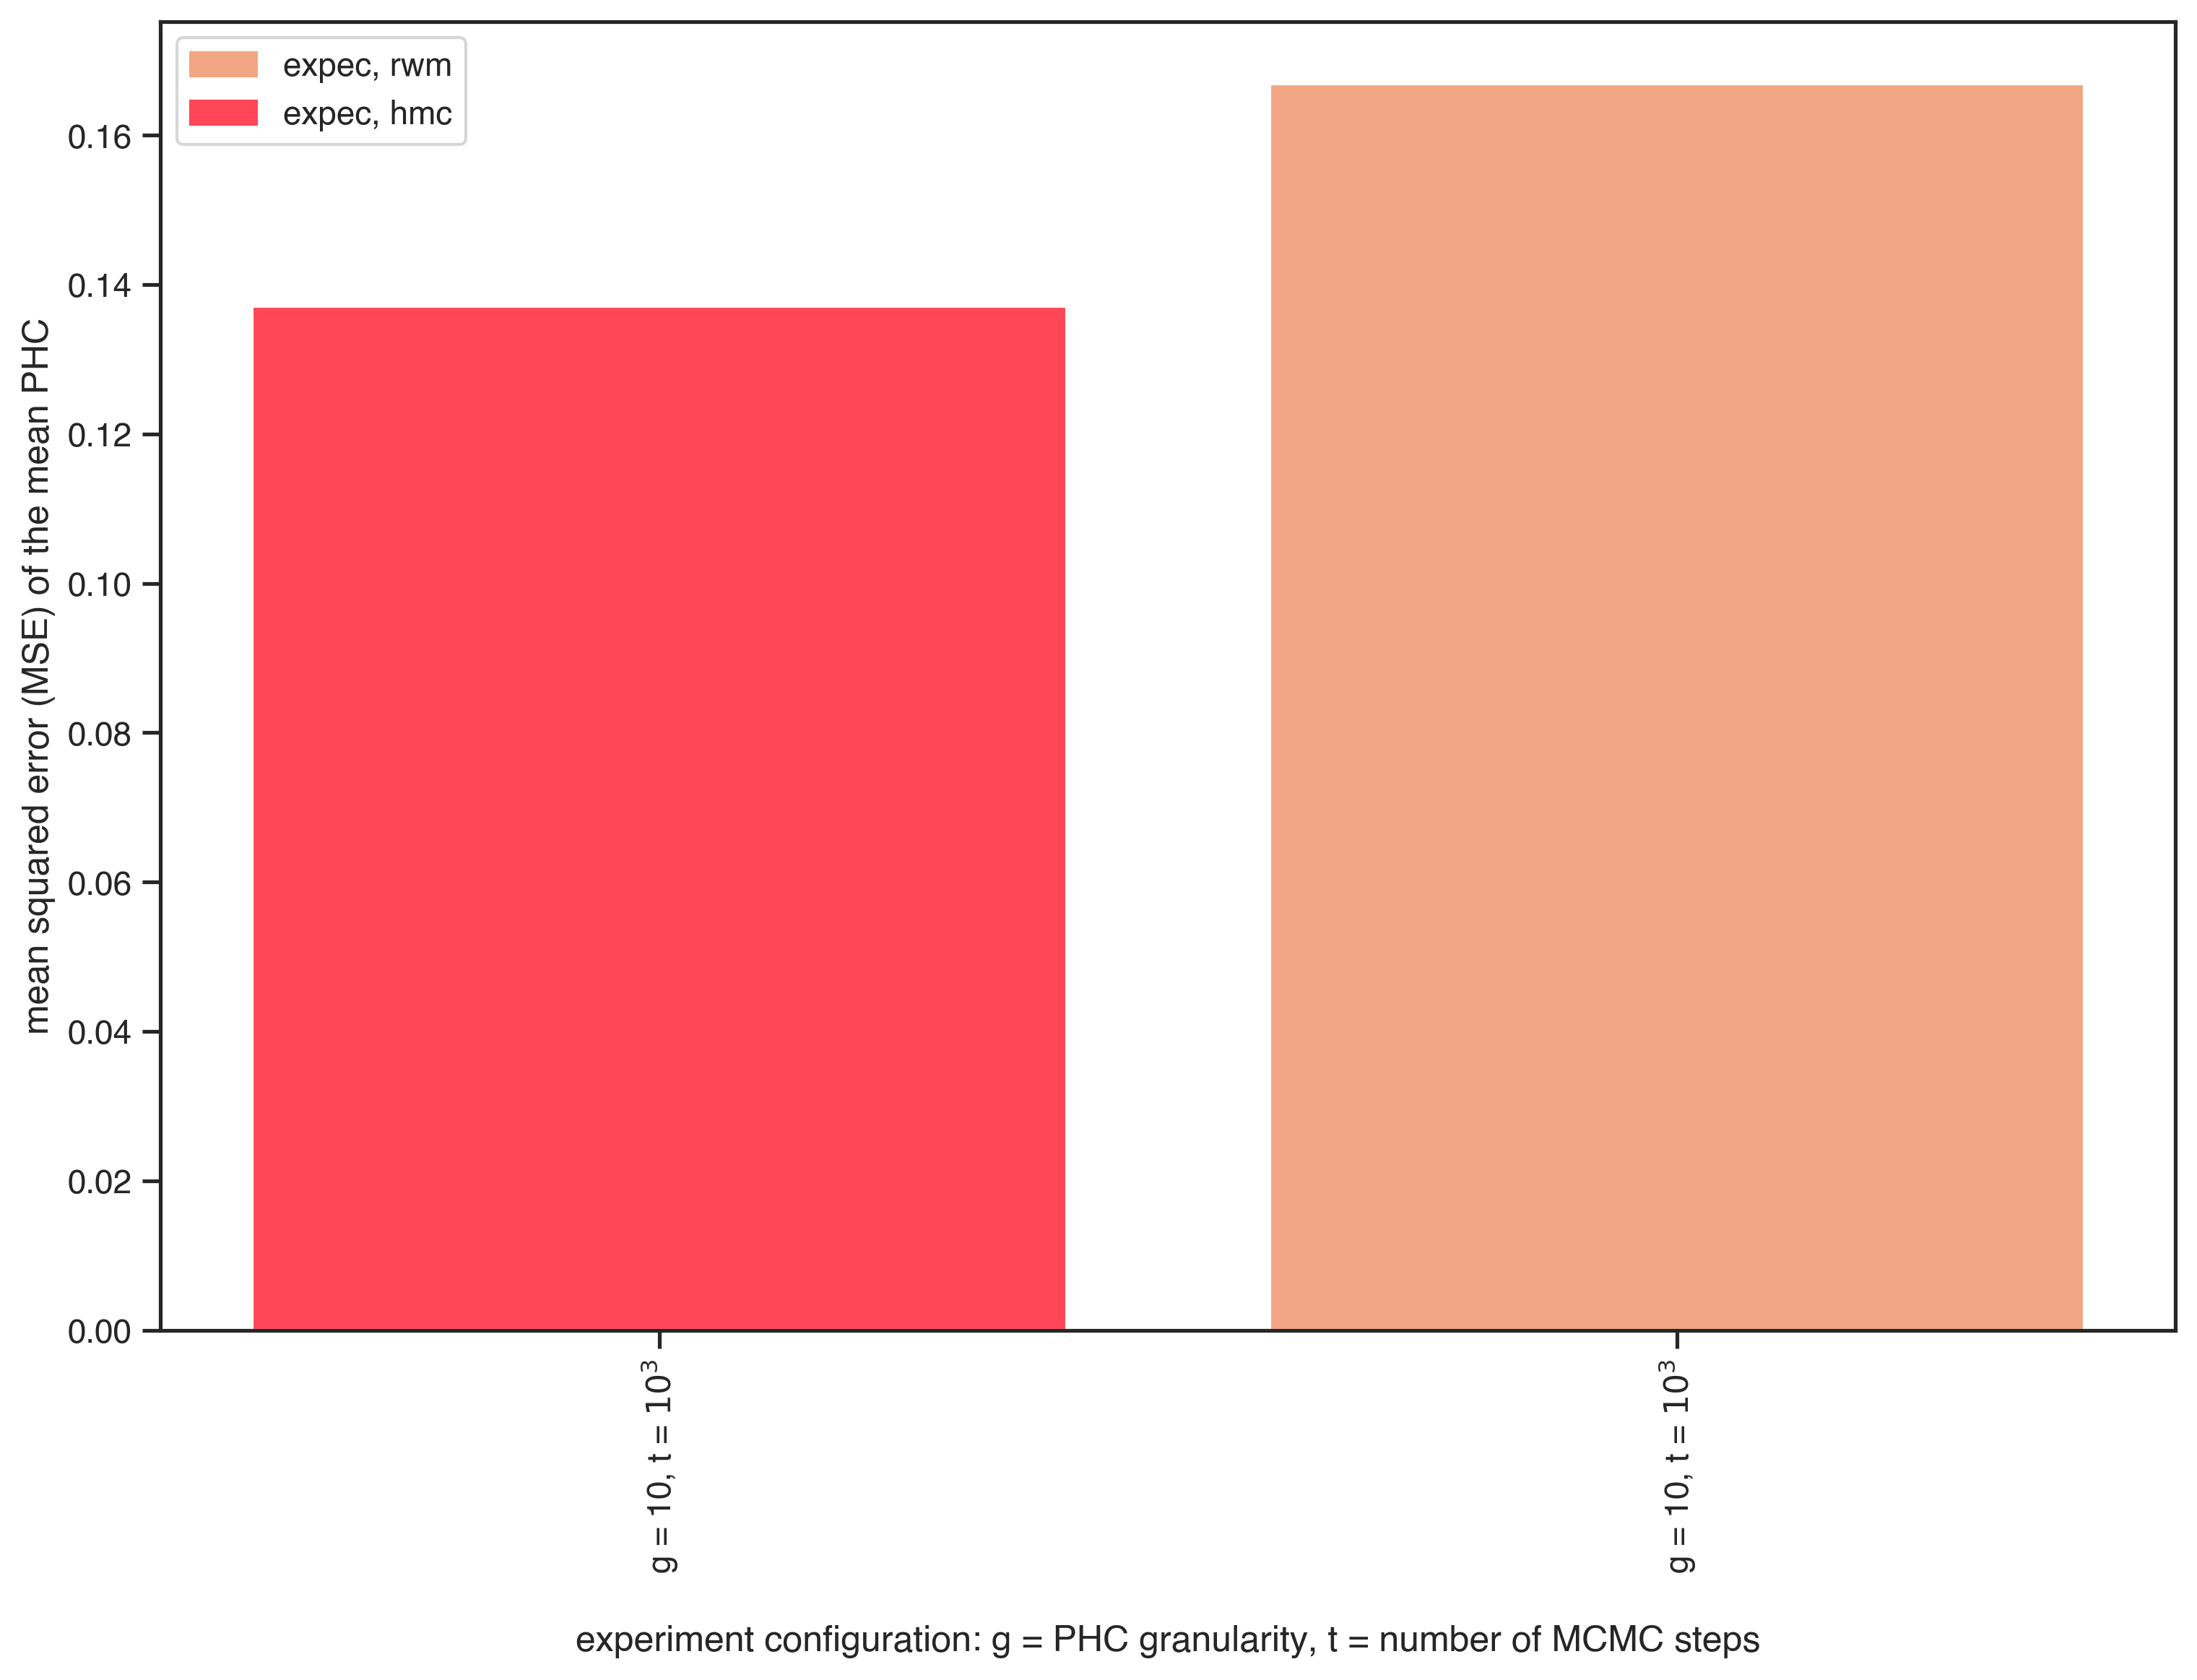
\includegraphics[width=0.75\linewidth]{figures/5_3_mean_mse.png}
 \caption{MSE of the Mean PHC of the Configurations' DVM on the $d_5 \times v_3$ Election}
 \label{fig:5_3_mean_mse}
\end{figure}

\begin{figure}[ht]\centering
 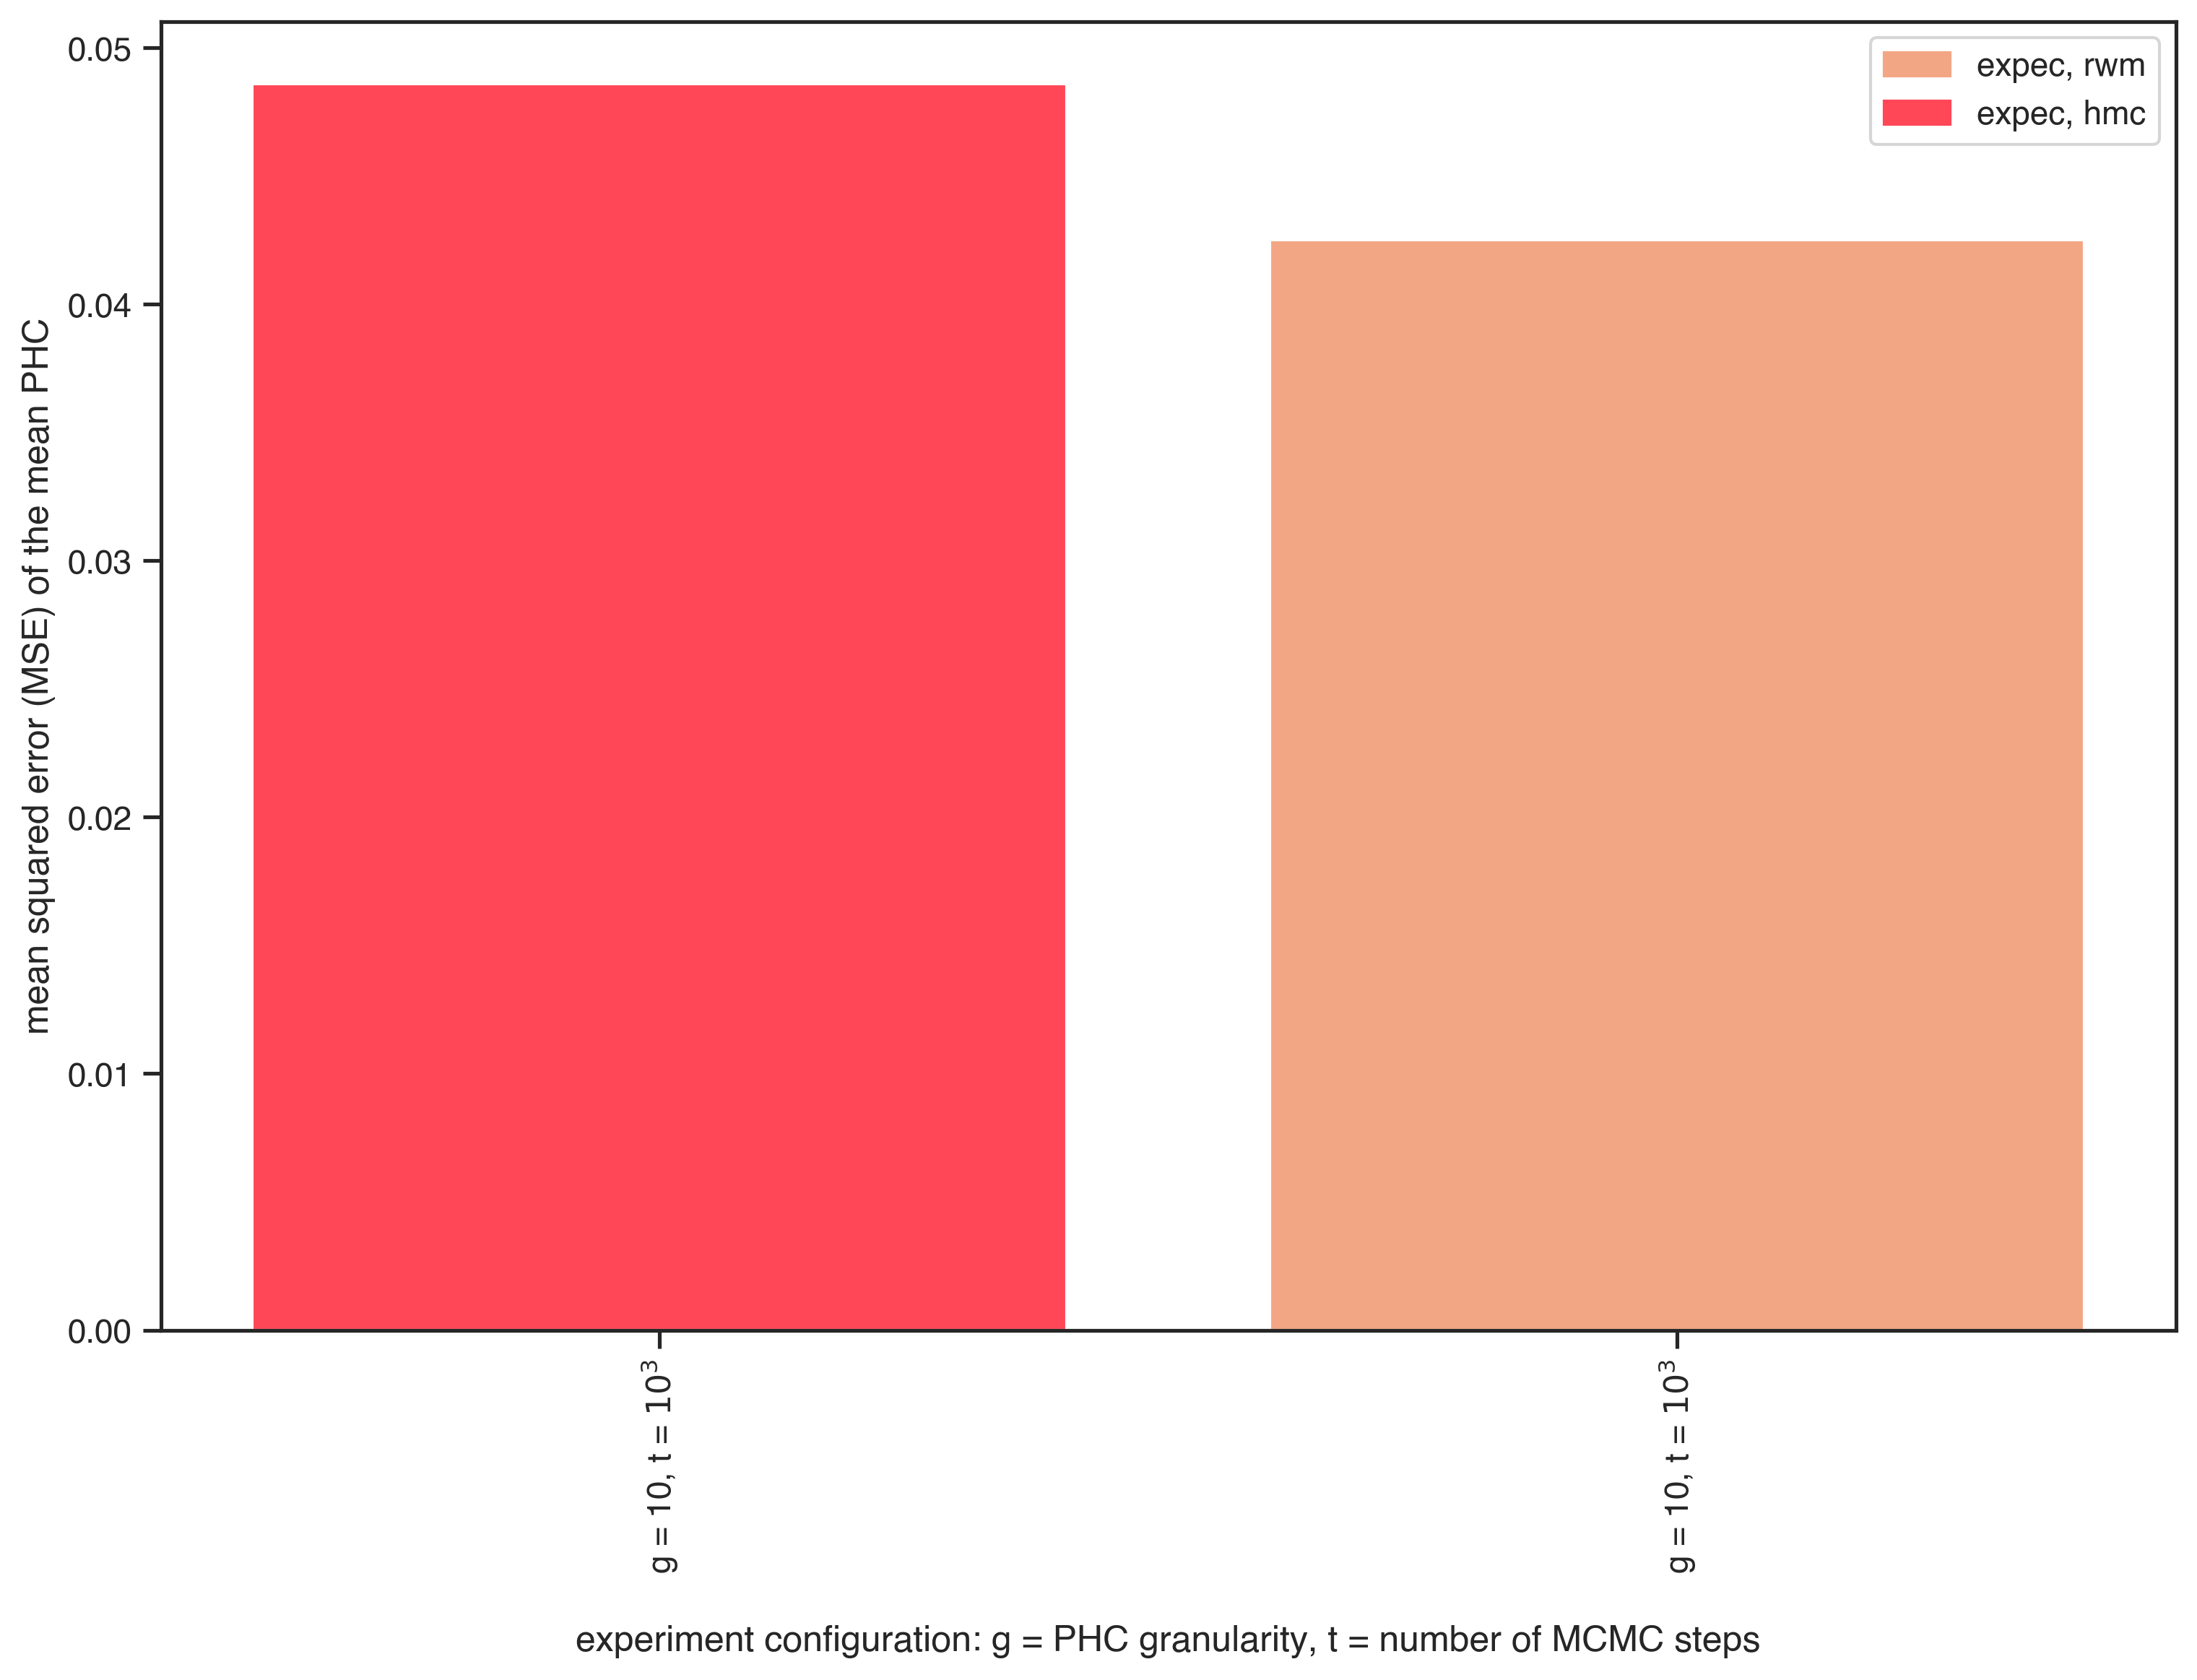
\includegraphics[width=0.75\linewidth]{figures/5_4_mean_mse.png}
 \caption{MSE of the Mean PHC of the Configurations' DVM on the $d_5 \times v_4$ Election}
 \label{fig:5_4_mean_mse}
\end{figure}

\begin{figure}[ht]\centering
 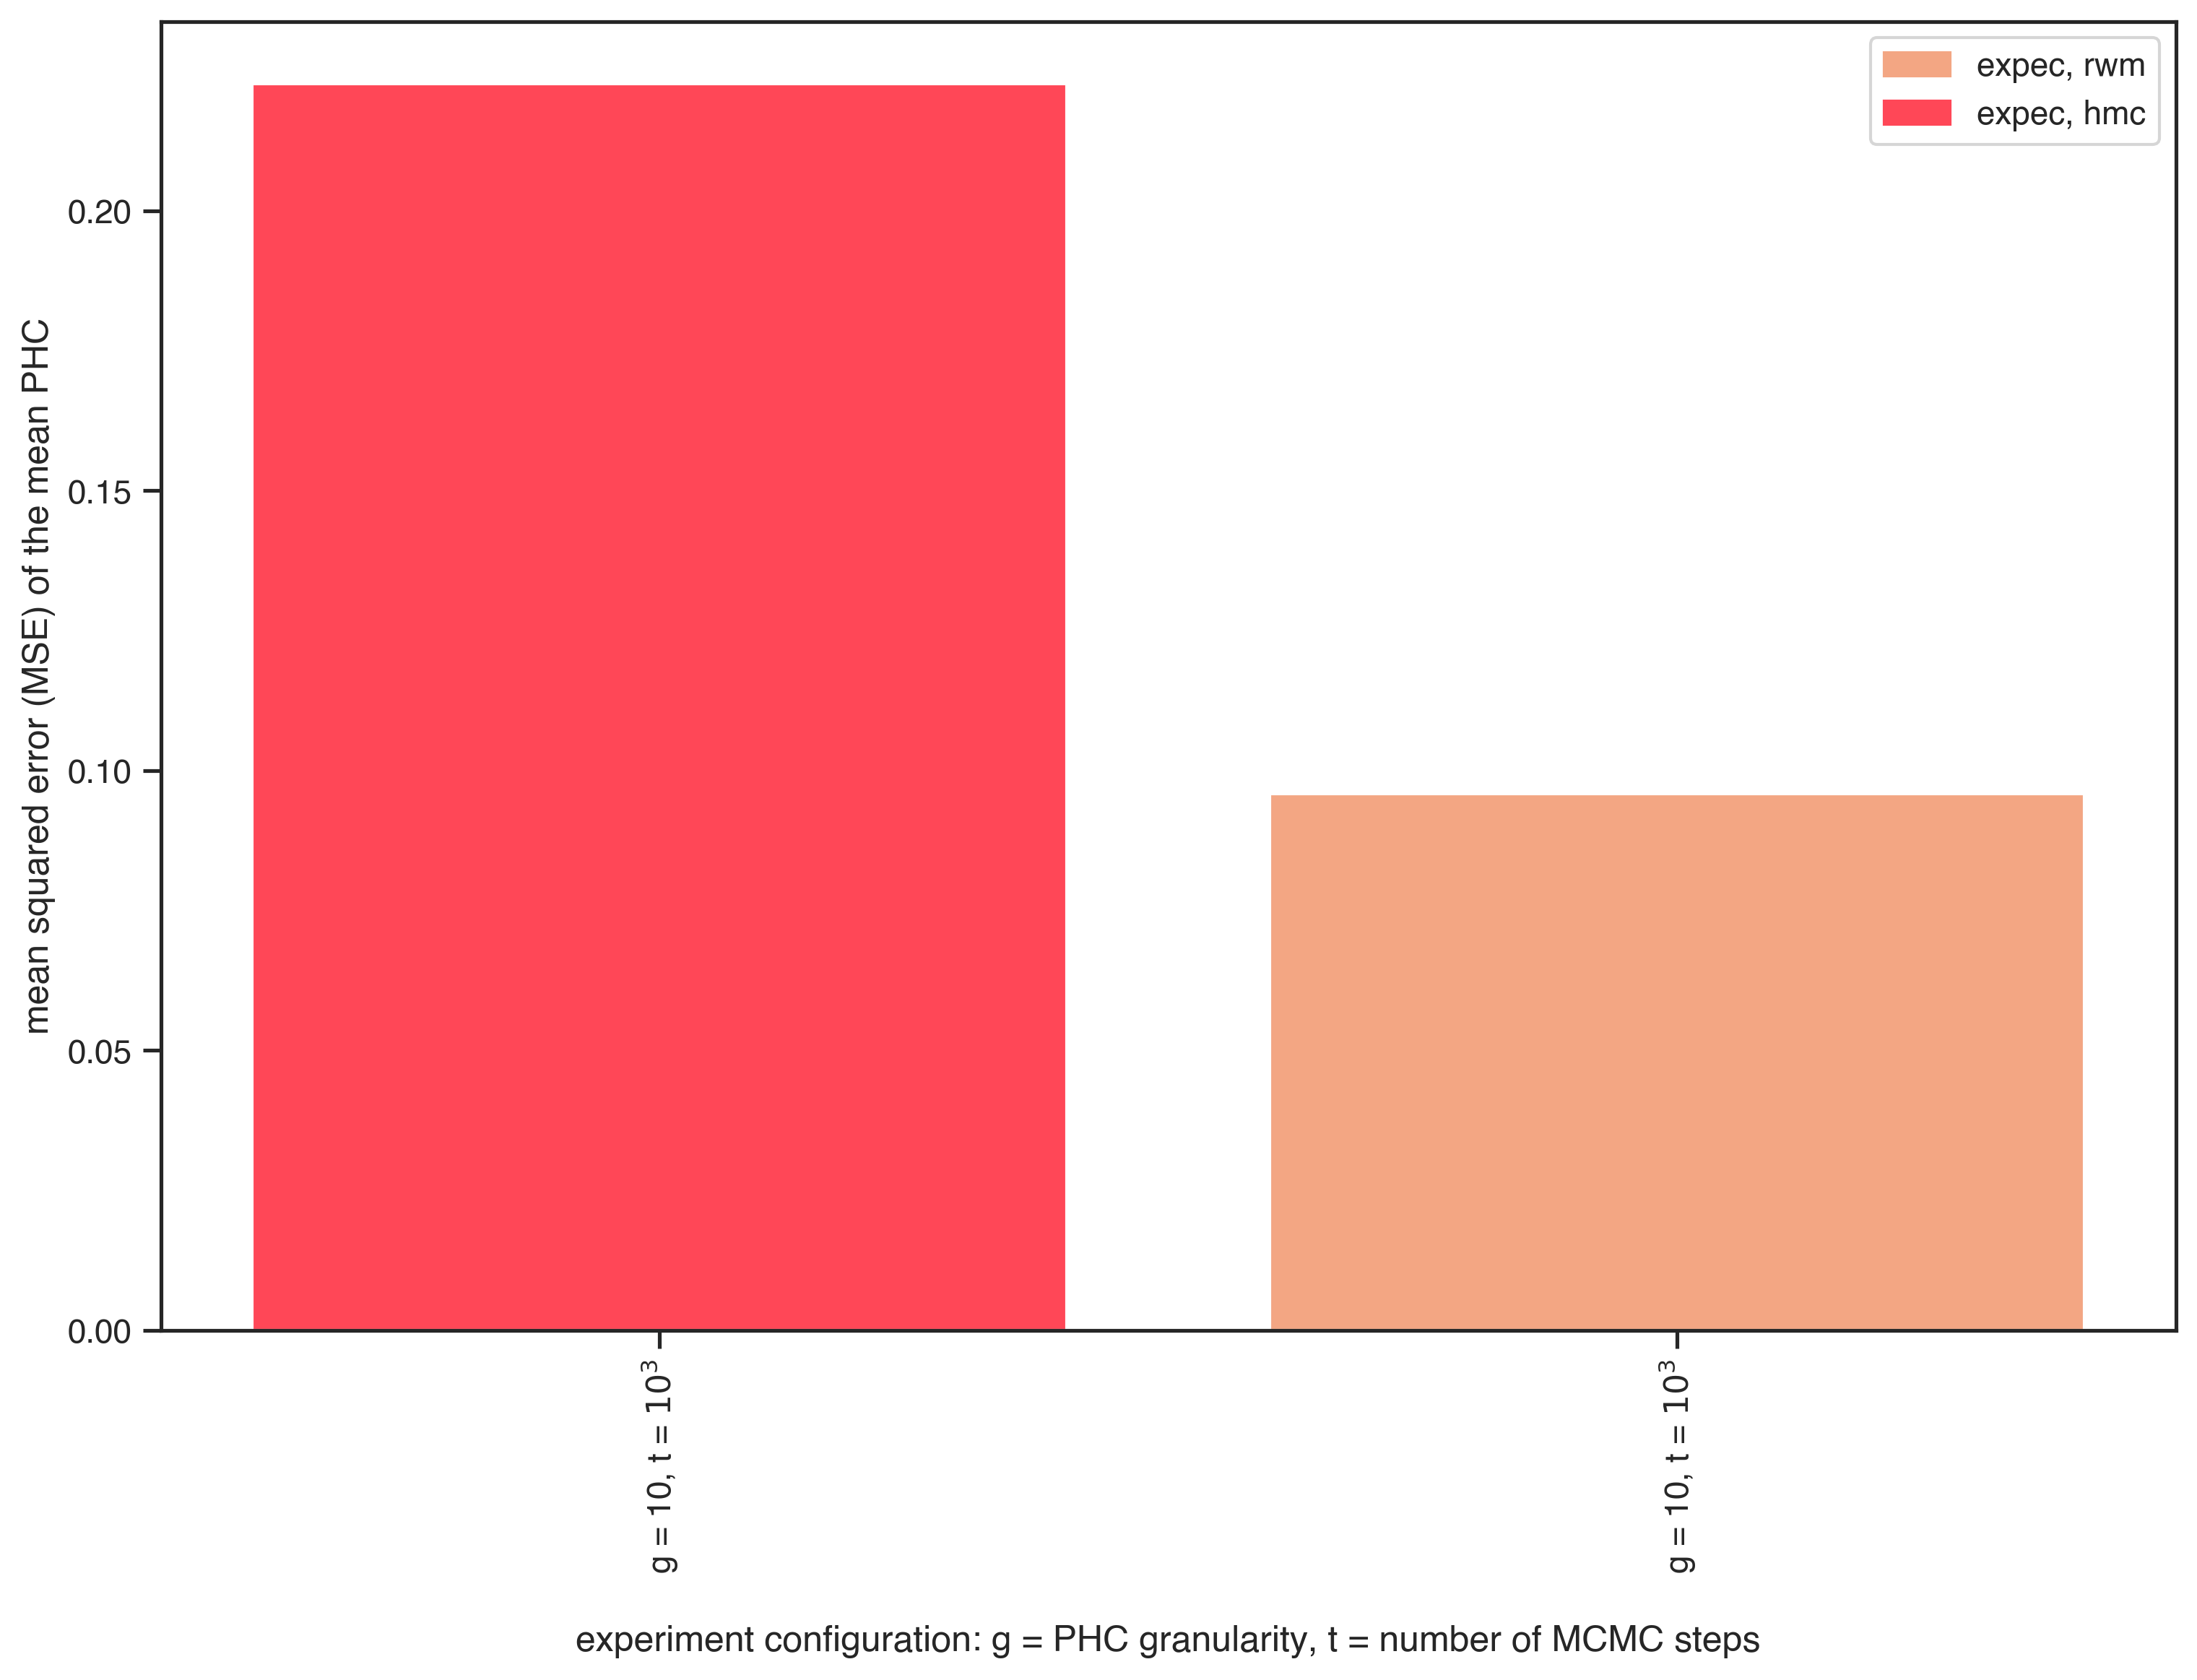
\includegraphics[width=0.75\linewidth]{figures/6_3_mean_mse.png}
 \caption{MSE of the Mean PHC of the Configurations' DVM on the $d_6 \times v_3$ Election}
 \label{fig:6_3_mean_mse}
\end{figure}

\begin{figure}[ht]\centering
 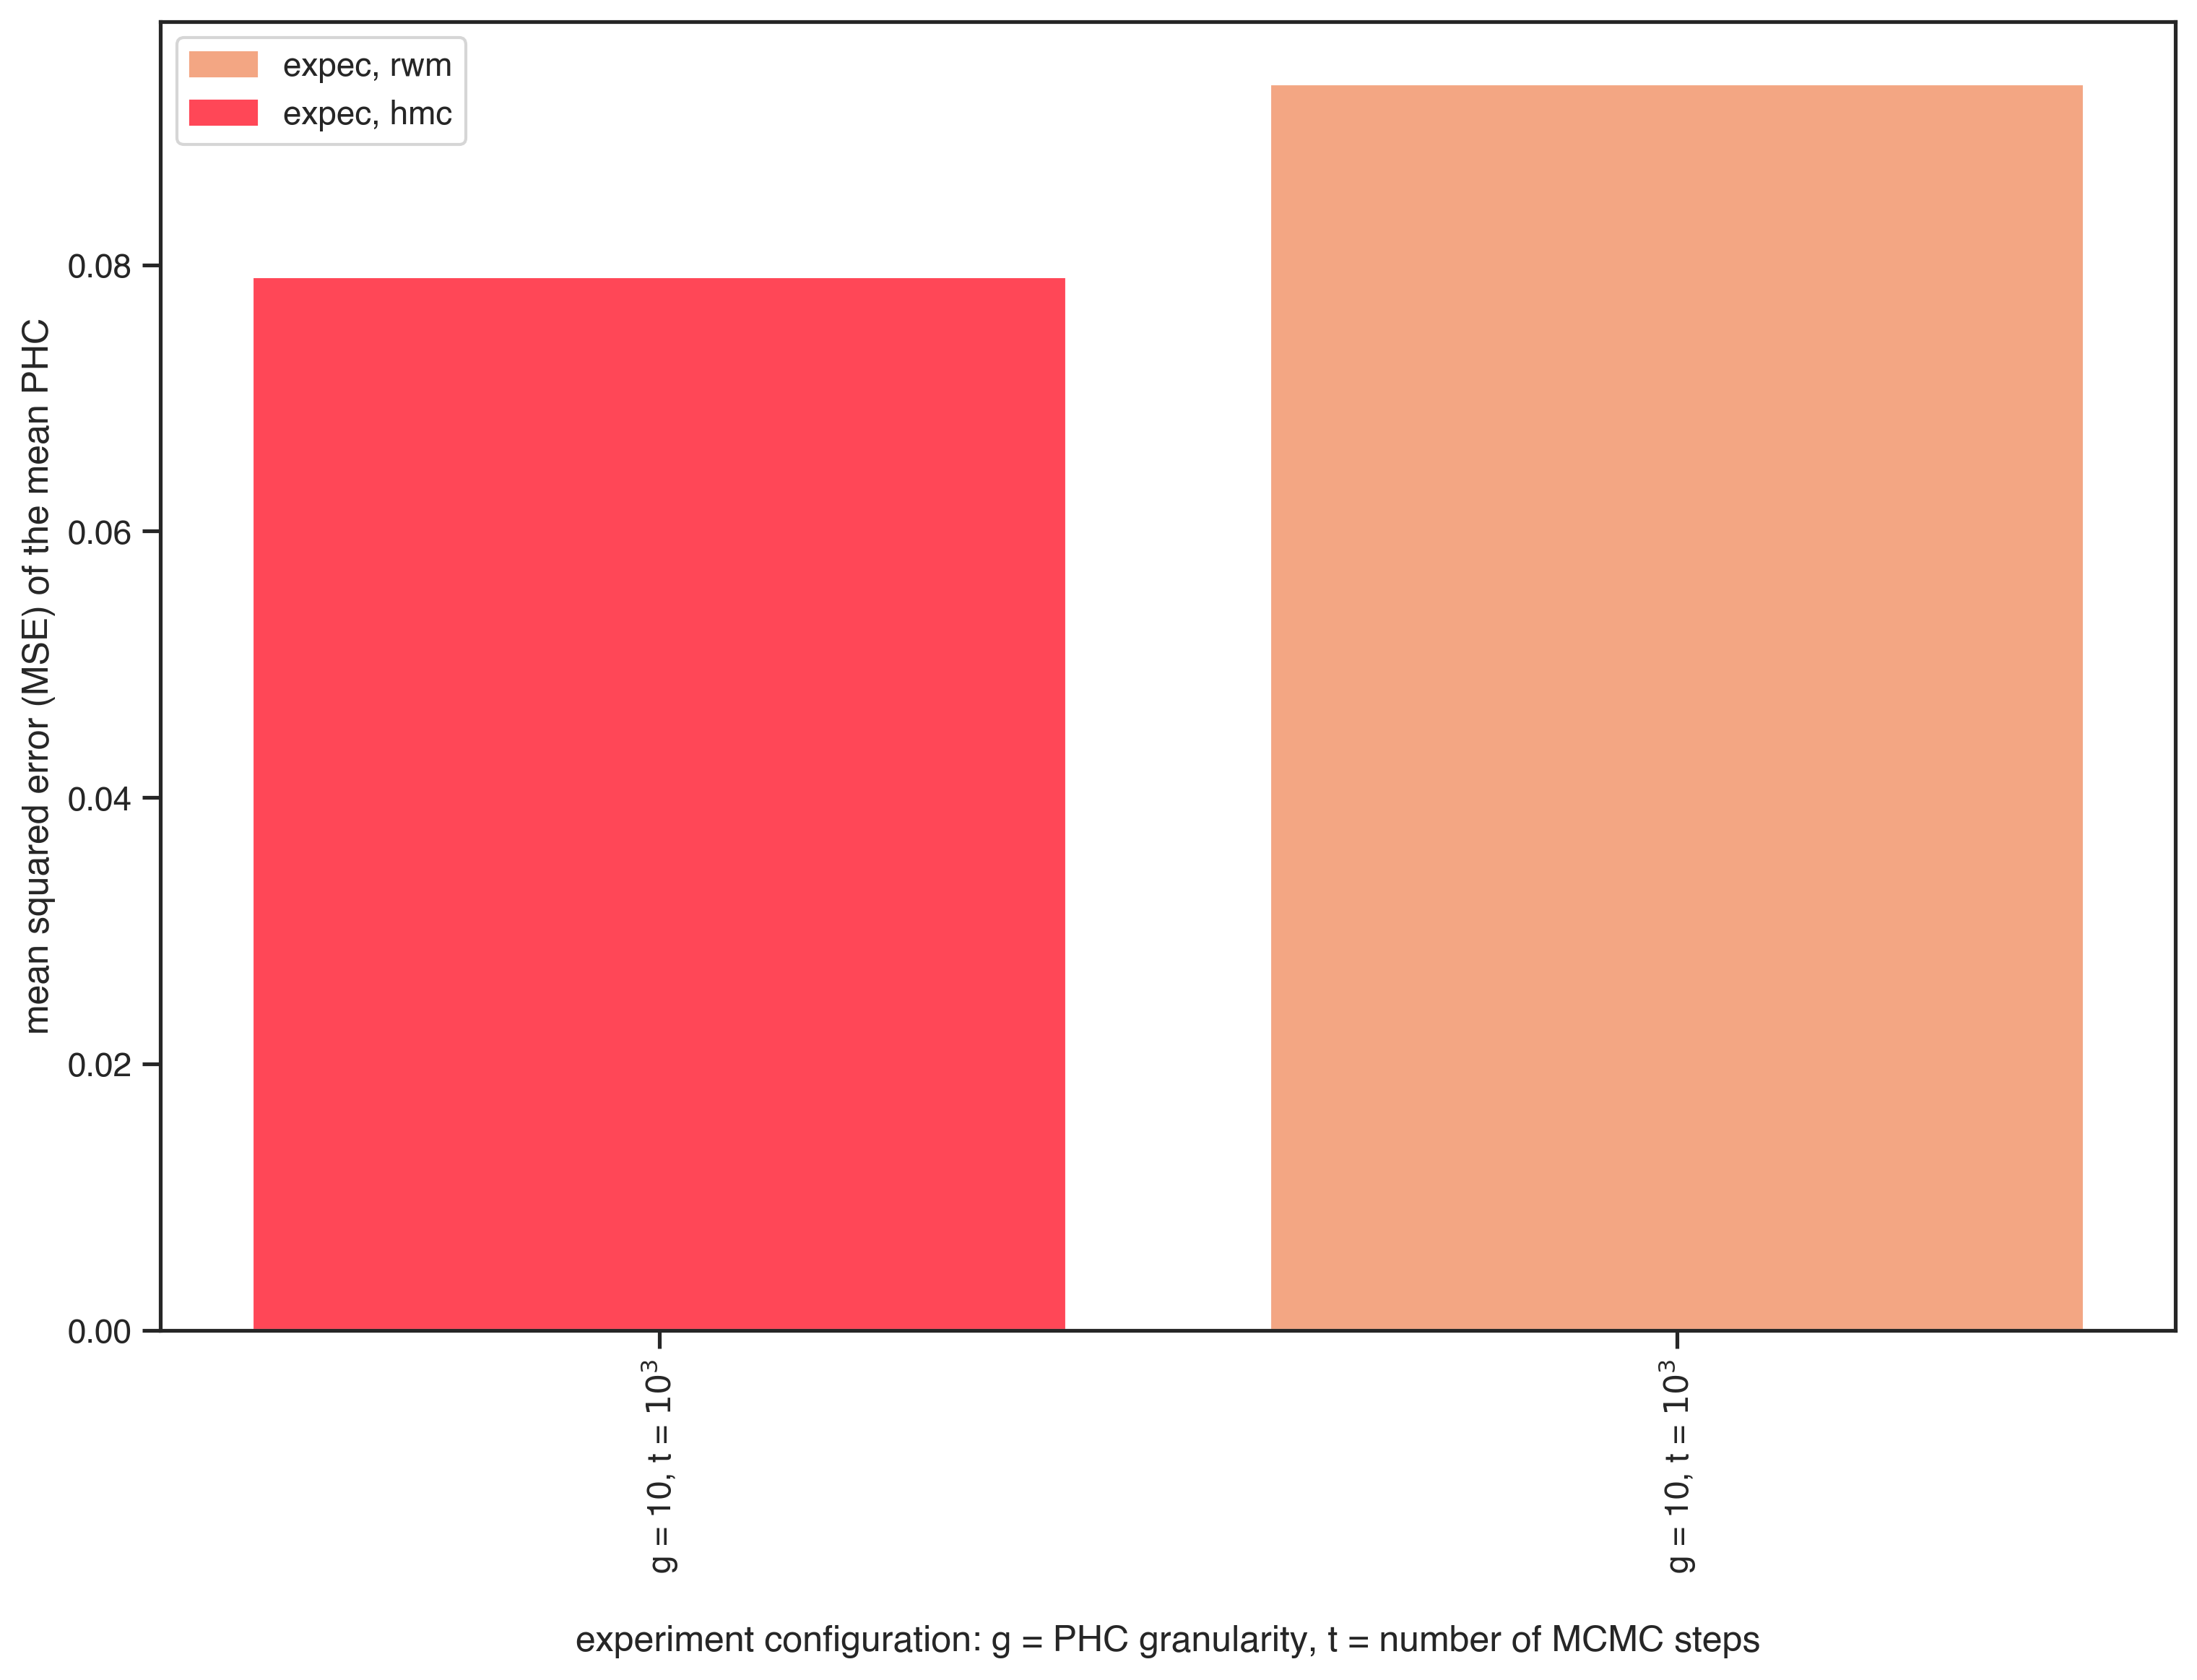
\includegraphics[width=0.75\linewidth]{figures/6_4_mean_mse.png}
 \caption{MSE of the Mean PHC of the Configurations' DVM on the $d_6 \times v_4$ Election}
 \label{fig:6_4_mean_mse}
\end{figure}
